% Este archivo es parte de la memoria del proyecto fin de carrera
% de Aarón Bueno Villares. Protegida bajo la licencia GFDL.
%
% Para más información, la licencia completa viene incluida en el
% fichero fdl-1.3.tex
%
% Fuente tomada del PFC 'DSMemorizer' de Diego Barrios Romero, a su vez
% tomada del PFC 'libgann' de Francisco Javier Vázquez Púa, a su vez 
% tomada de la plantilla LaTeX para la realización de Proyectos Final 
% de Carrera de Pablo Recio Quijano.

% Copyright (C) 2008 Francisco Javier Vázquez Púa
% Copyright (C) 2009 Pablo Recio Quijano
% Copyright (C) 2009 Diego Barrios Romero

% Copyright (C) 2010 Aarón Bueno Villares

\documentclass[a4paper,12pt]{book}

\usepackage{./estilos/estiloBase}
\usepackage{./estilos/colores}
\usepackage{./estilos/comandos}

\setcounter{secnumdepth}{3}
\setcounter{tocdepth}{3}
\setlength{\parskip}{1em}

\begin{document}

%%%%%%%%%%%%%%%%%%%%%%%%%%%%%%%%%%%%
%%       Preámbulos
%%%%%%%%%%%%%%%%%%%%%%%%%%%%%%%%%%%%
% Este archivo es parte de la memoria del proyecto fin de carrera
% de Aarón Bueno Villares. Protegida bajo la licencia GFDL.
% Para más información, la licencia completa viene incluida en el
% fichero fdl-1.3.tex
%
% Fuente tomada del PFC 'DSMemorizer' de Diego Barrios Romero, a su vez
% tomada del PFC 'libgann' de Francisco Javier Vázquez Púa, a su vez tomada de la plantilla LaTeX para
% la realización de Proyectos Final de Carrera de Pablo Recio Quijano.

% Copyright (C) 2008 Francisco Javier Vázquez Púa
% Copyright (C) 2009 Pablo Recio Quijano
% Copyright (C) 2009 Diego Barrios Romero

% Copyright (C) 2009 Aarón Bueno Villares

\pagestyle{empty}
\begin{titlepage}

  \begin{center}

   
\includegraphics[scale=0.2]{imagenes/logo_uca.png} 

    \vspace{2.0cm}

    \LARGE{\textbf{ESCUELA SUPERIOR DE INGENIERÍA}} \\

    \vspace{1.0cm}

    \Large{\textbf{INGENIERÍA TÉCNICA EN INFORMÁTICA DE SISTEMAS}} \\

    \vspace{3.0cm}

    \Large{\gomf:\\ Simulador de batallas fantásticas} \\

    \vspace{2.0cm}

    \Large{Aarón Bueno Villares} \\

    \vspace{0.5cm}

    \large{\today}

  \end{center}
\end{titlepage}

\cleardoublepage

% Este archivo es parte de la memoria del proyecto fin de carrera
% de Aarón Bueno Villares. Protegida bajo la licencia GFDL.
% Para más información, la licencia completa viene incluida en el
% fichero fdl-1.3.tex
%
% Fuente tomada del PFC 'DSMemorizer' de Diego Barrios Romero, a su vez
% tomada del PFC 'libgann' de Francisco Javier Vázquez Púa, a su vez tomada de la plantilla LaTeX para
% la realización de Proyectos Final de Carrera de Pablo Recio Quijano.

% Copyright (C) 2008 Francisco Javier Vázquez Púa
% Copyright (C) 2009 Pablo Recio Quijano
% Copyright (C) 2009 Diego Barrios Romero

% Copyright (C) 2009 Aarón Bueno Villares

\pagestyle{empty}
\begin{center}

  
\includegraphics[scale=0.2]{./imagenes/logo_uca.png} \\

  \vspace{2.0cm}

  \Large{ESCUELA SUPERIOR DE INGENIERÍA} \\

  \vspace{1.0cm}

  \large{INGENIERO TÉCNICO EN INFORMÁTICA DE SISTEMAS} \\

  \vspace{2.0cm}

  \large{\gomf:\\ Simulador de batallas fantásticas} \\

  \vspace{1.0cm}

\end{center}

\begin{itemize}
\item \large{Departamento: Lenguajes y sistemas informáticos}
\item \large{Director del proyecto: Manuel Palomo Duarte}
\item \large{Autor del proyecto: Aarón Bueno Villares}
\end{itemize}

\vspace{1.0cm}

\begin{flushright}
  \large{Cádiz, \today} \\

  \vspace{2.5cm}

  \large{Fdo: Aaron Bueno Villares}
\end{flushright}

\cleardoublepage

\frontmatter 
\pagestyle{plain}
% Este archivo es parte de la memoria del proyecto fin de carrera
% de Aarón Bueno Villares. Protegida bajo la licencia GFDL.
% Para más información, la licencia completa viene incluida en el
% fichero fdl-1.3.tex
%
% Fuente tomada del PFC 'DSMemorizer' de Diego Barrios Romero, a su vez
% tomada del PFC 'libgann' de Francisco Javier Vázquez Púa, a su vez tomada de la plantilla LaTeX para
% la realización de Proyectos Final de Carrera de Pablo Recio Quijano.

% Copyright (C) 2008 Francisco Javier Vázquez Púa
% Copyright (C) 2009 Pablo Recio Quijano
% Copyright (C) 2009 Diego Barrios Romero

% Copyright (C) 2009 Aarón Bueno Villares

\section*{Licencia}

Este documento ha sido liberado bajo Licencia GFDL 1.3 (GNU Free
Documentation License). Se incluyen los términos de la licencia en
inglés al final del mismo.

Copyright (c) 2010 Aarón Bueno Villares.

Permission is granted to copy, distribute and/or modify this document
under the terms of the GNU Free Documentation License, Version 1.3 or
any later version published by the Free Software Foundation; with no
Invariant Sections, no Front-Cover Texts, and no Back-Cover Texts. A
copy of the license is included in the section entitled "GNU Free
Documentation License".

\cleardoublepage

\tableofcontents
\listoffigures
\listoftables

%%%%%%%%%%%%%%%%%%%%%%%%%%%%%%%%%%%%
%%      Cuerpo
%%%%%%%%%%%%%%%%%%%%%%%%%%%%%%%%%%%%
\mainmatter

\pagestyle{plain}

% Este archivo es parte de la memoria del proyecto fin de carrera
% de Aarón Bueno Villares. Protegida bajo la licencia GFDL.
% Para más información, la licencia completa viene incluida en el
% fichero fdl-1.3.tex

% Copyright (C) 2010 Aarón Bueno Villares

\chapter{Introducción}
\label{chap:introduccion}

Existen muchos videojuegos de estrategia y táctica bélica tanto en el
mercado como en el mundo libre, pero debido al atractivo de los nuevos
avances en diseño 3D y el paradigma del juego en tiempo real, se está
dejando a los juegos por turnos en un segundo plano. Cuando estamos
ante un juego de táctica militar, en general, hay muchísimos factores
a tener en cuenta a cada paso del juego, desde la posición de los
efectivos representativos de tu ejército, hasta el encaramiento de las
unidades, pasando por la situación de los elementos de escenografía o
los posibles flancos libres del enemigo. Todo esto, obviamente, no
puede ser abarcado por un solo jugador humano en tiempo real,
perdiendo gran parte del control sobre la dinámica de su propio
ejército.

Este juego pretende revivir el interés hacia los juegos por turnos
haciendo resaltar todos los aspectos que en una guerra ocurren y
aumentando el atractivo del mismo al darle un contexto medieval y
fantástico. 

\section{Motivación}
Durante mi estancia en bachillerato, conocí \textit{Warhammer Fantasy
  Battles} -abreviadamente, \textit{WF}-, propiedad de la empresa
\emph{Games Workshop}. El paradigma de juego era para
mí tan novedoso como atractivo. Existía una gran comunidad de
jugadores seguidores de este juego a mi alrededor, y además destacaba
fuertemente entre otros juegos de la misma temática (de hecho, era el
único popularmente conocido).

Los precios de miniaturas, pinturas, pinceles, reglamentos y elementos
de escenografía eran altos, pero la calidad, madurez, entretenimiento,
progreso, versatilidad y oportunidades que se ofrecían lo
compensaban.

Con el paso de los años, la compañia orientó el juego a un público
cada vez mas infantil, con el consecuente ataque a los bolsillos de
padres y madres, en vez de a los bolsillos de los jóvenes,
generalmente con menor disponibilidad económica. En resumen, el precio
escapó a mis posibilidades. Las reglas y la forma de juego también se
simplificó e infantilizó. La calidad de las miniaturas también se
redujo (aunque los diseños eran cada vez mas impresionantes). Tampoco
acompañaba el tiempo disponible de dedicación, pues con la edad se
empiezan a asumir otro tipo de responsabilidades. Y no fui el único
que corrió la misma suerte. Hoy en día, ninguno de los jugadores que
conocí continúan manteniendo su hobby, y al igual que yo, guardan sus
miniaturas en cajas y maletines protegidas con algodón.

El siguiente paso obvio fue buscar alguna alternativa digital que
capturara exáctamente la esencia de \textit{WF} para poder seguir
diseñando y ejecutando tácticas  y enfrentándolas a otros jugadores,
con mayor comodidad y menor esfuerzo y coste. Dicha búsqueda resultó
una quimera, pues no existía tal alternativa. Incluso en foros de
videojuegos en algún lugar de internet encontré a gente que también
buscaba y preguntaba lo mismo que yo, desde diversas partes del mundo
(al menos en el mundo de habla hispana).
  
Pasaron dos años desde aquel entonces hasta que me llegó la hora de
decidir que PFC realizar, y, por un afortunado comentario de
\textit{Manuel Palomo Duarte}, acerca del proyecto de otro alumno
sobre otro juego de la misma empresa, el conocido y afamado
\emph{Blood Bowl}, durante la clase de diseño de videojuegos, me di
cuenta que quizás yo debía ser la persona responsable de construir
aquello que con tanta esperanza buscábamos (puesto que era el único de
entre aquellos amigos jugadores de \textit{WF} que empezó a estudiar
informática en la universidad y tenía capacidades suficientes para
crear un videojuego modesto). Y así fue como nació \gomf.

\section{Alcance}
Existen muchos jugadores de juegos de mesa que recrean batallas del
rol de \gomf, obligados por las empresas productoras de estos juego a
comprar un gran número de miniaturas de alto precio para poder
disfrutar de su hobby. Con este proyecto se pretende soslayar estas
dificultades con un producto de calidad que recree estas situaciones
para que estos jugadores puedan competir contra otros y poner a prueba
sus capacidades tácticas, gratuitamente y con un control automático de
las reglas sobre las que se construye el juego. Además al ser el juego
de licencia pública y gratuita, se favorecen las posibilidades de una
rápida expansión y la llegada a muchas manos (se espera que en un
futuro al menos, todo jugador o ex-jugador de \textit{WF} llege a
conocerlo).

Y la criatura se llamará \gomf, y será la culminación final de estas ideas.

\section {Sobre este documento}
Este documento es la memoria de la realización del proyecto fin de
carrera de la titulación \emph{Ingeniería Técnica en Informática de
  Sistemas} (abreviadamente ITIS), de la Universidad de Cádiz, de
\textit{Aarón Bueno Villares} (un servidor).

El documento se organiza en los siguientes capítulos:

\begin{enumerate}
\item \textit{Introducción}: Es el capítulo que actualmente estás
  leyendo. Da una somera introducción a la idea que da título al
  proyecto y a la memoria emergente a partir del mismo. 
\item \textit{Calendario}: Organización temporal de desarrollo del
  proyecto.
\item \textit{Especificación de requisitos del sistema}:
  Especificación y establecimiento de la funcionalidad que ofrecerá el
  software.
\item \textit{Análisis y diseño del sistema}: Descripción del proceso
  de desarrollo del software.
\item \textit{Principales problemas de implementación}: Principales
  problemas de implementación encontrados en la implementación
  efectiva del software.
\item \textit{Pruebas}: Metodología usada para las pruebas de
  verificación del software.
\item \textit{Herramientas}: Herramientas usadas como apoyo en la
  realización del software.
\item \textit{Conclusiones}: Experiencia, resultado, nuevas ideas y en
  general, toda aquella sensación experimentada durante la realización
  del proyecto.
\item \textit{Diversos apéndices}: Manual del usuario, reglamento de
  \gomf, bibliografía, licencia \emph{GFDL} y licencia \emph{GPL}. 
\end{enumerate}

% Este archivo es parte de la memoria del proyecto fin de carrera
% de Aarón Bueno Villares. Protegida bajo la licencia GFDL.
%
% Para más información, la licencia completa viene incluida en el
% fichero fdl-1.3.tex

% Copyright (C) 2010 Aarón Bueno Villares

\chapter{Desarrollo del sistema}
\label{chap:desarrollo}

El primer paso mas importante antes de comenzar a crear verdaderamente
\gomf, es planificar su desarrollo, indentificando sus partes, y,
sobre todo, forjar definitivamente qué vamos a entender por \gomf, es
decir, qué hará exáctamente y cómo, y de cara al usuario, \gomf.

La búsqueda de la respuesta a esta pregunta ha sido el mas fiel
acompañante del proceso de desarrollo, pues no terminó de contestarse
hasta su finalización, pues como ya advierte la ingeniería del software, esta
tarea no es nada sencilla. Y además, cuando a uno se le ofrece la
oportunidad de \emph{hacer lo que  quiera}, solo un conformista se
declarará impasible ante esta situación. Es una vía abierta para
desplegar sus artes y de demostrar a los demás, como excusa para
demostrarse a sí mismo, sus propias capacidades. En este punto, las
ideas flotan, emergen y nadan en un mar caótico de realizaciones
personales a las que difícilmente se les puede poner orden.

El proceso de diseño y la implementación consecuente se fue realizando
a medida que se aclaraba la respuesta a la primera pregunta. Por
tanto, podemos decir que nuestro proyecto se ha realizado bajo una
modelo de desarrollo iterativo incremental, donde, por lo general, a
cada nueva iteración se definían (o redefinían) los siguientes
aspectos a desarrollar, junto a la experiencia ganada en los ciclos
anteriores. También el propio reglamento fue adaptándose a las
dificultades encontradas en el diseño y la implementación. La
descripción en esta memoria del proceso de desarrollo reflejará esta
historia.

La orientación a objetos ha sido el enfoque elegido para realizar el
desarrollo de nuestro juego.

\newpage
% Este archivo es parte de la memoria del proyecto fin de carrera
% de Aarón Bueno Villares. Protegida bajo la licencia GFDL.
%
% Para más información, la licencia completa viene incluida en el
% fichero fdl-1.3.tex

% Copyright (C) 2010 Aarón Bueno Villares

\section{Calendario}
\label{sec:calendario}

Aquí se describirá mas concisamente el contenido de cada una de estas
iteraciones de desarrollo.

Hay que advertir que durante todo el tiempo que ha
durado la confección de este proyecto no me he dedicado únicamente al
mismo. Mientras, continuaba las asignaturas que me quedaban de la
titulación técnica y luego comencé a cursar asignaturas del segundo
ciclo. Así que, en muchas ocasiones durante la realización del
proyecto me he visto obligado a pausar el desarrollo del mismo para
dedicarme enteramente a las asignaturas, lo que explica en parte su
larga duración.

En la figura \ref{fig:gantt} se muestra el diagrama de Gantt
correspondiente al calendario de nuestro proyecto.

\subsection{Definición inicial}
Cuando decidí realizar este proyecto, solo tenía una idea vaga de qué
iba a desarrollar. Tenía un propósito y un objetivo, como ya se
advirtió en el capítulo \ref{chap:introduccion}, pero no
sabía de que forma concreta esas ideas tomarían definitivamente
su forma. El primer ciclo de desarrollo corresponde a este periodo de
reflexión inicial, que fecundó en un reglamento que serviría como
punto de partida para el desarrollo consecuente.

En esta iteración se definió la categoría del juego, tras conocer e
investigar los taxones en los que se clasifican los videojuegos, se
conoció algo de la historia del paradigma de juegos de mesa que estaba
implementando para obtener inspiración de diversos reglamentos de
diversos juegos históricos de táctica militar (aunque mi mayor fuente
de inspiración siempre ha sido el reglamento de \emph{WF} por
ser el reglamento que mejor conozco), y se exploró mas concisamente
acerca de si efectivamente mi juego sería el único videojuego de esta
corte, explorando muchas páginas webs dedicadas a la recopilación de
información sobre videojuegos tanto clásicos como modernos. Así que
podemos decir que este primer ciclo también contiene una etapa de
documentación.

También se estuvo decidiendo que \emph{paradigma} de interfaz
usaríamos, si el videojuego sería 3D, isométrico o un juego 2D
plano. Al final me decanté por la última opción, pues no tenía las
artes suficientes para crear los modelos gráficos que necesitaría para
las dos primeras opciones.

Por último, junto a los demás aspectos, se configuró un reglamento
inicial de \gom.

\subsection{Arquitectura general del sistema}
Esta iteración contituye el primer ciclo de diseño, que a su vez es el mas
importante, pues se estableció la arquitectura general del sistema
(véase \ref{sec:diseno}), es decir, como organizaríamos las clases
principales y de mas alto nivel de abstracción que conformarían la
resolución del problema de implementar ese primer reglamento.

\subsection{Fase de movimiento}
La primera fase que se diseñó y luego implementó fue la fase de
movimiento. En su intento de implementación, se rediseñó el reglamento
en gran medida, pues llegé a comprender la gran complejidad que
contenía la versión inicial. Este ciclo contituye casi el 80\% del
desarrollo del sistema, sobre todo por las dificultades en establecer
los cálculos correctos del \emph{gestor de escenarios} (véase
\ref{sec:diseno}), que contenía mucha matemática y geometría.

\subsection{Gestor de interfaz}
Conjuntamente al ciclo anterior, se fue implementando la interfaz
necesaria para poder visualizar las implementaciones del gestor de
movimiento. Esta primera versión del gestor de interfaz fue la que
configuró el aspecto gráfico de las batallas.

\subsection{Fase de combate}
Una vez implementada la fase de movimiento, se podía comenzar a
desarrollar la fase de combate, pues sin la primera, no se podía
desarrollar la segunda (para combatir, hace falta realizar
cargas, cosa que se hace en la fase de movimiento). Nuevamente, el
reglamento sufrió modificaciones en torno a los aspectos involucrados
en esta fase.

\subsection{Mejora de la interfaz}
En esta iteración o ciclo, el gestor de interfaz tomaría su forma
final. Ya no sería un simple \emph{visualizador de batallas}. Ahora
sería una interfaz de menús donde el usuario podía realizar varias
cosas, no solo jugar batallas.

Por ello, se añadió una herramienta para poder configurar ejércitos
desde el propio programa, que luego se podrían elegir desde el mismo
software para comenzar la partida. La creación de esta herramienta
propició una nueva linea de desarrollo que tiene autonomía por sí
misma.

También se dedicó un episodio importante a mejorar
la interfaz gráfica, añadiendo multitud de cambios, a ajustar las
fuentes, las imágenes, los ejércitos y los sonidos, y a realizar
modificaciones en la interfaz para adaptar los nuevos cambios e ideas.

\subsection{Fase de disparos y magia}
En esta iteración, se añadió al juego la fase de disparo, y también se
implementó la magia. La inclusión en el juego de los disparos y la
magia fue bastante sencilla, quizás gracias al buen diseño realizado en las
iteraciones anteriores.

\subsection{Memoria del proyecto}
Una vez terminado de programar el juego, se hizo la memoria del
proyecto. En realidad, esta memoria ya había ido realizándose
paulatinamente junto a las iteraciones anteriores, pero tras finalizar el
juego fue cuando me dediqué enteramente a su confección.

\begin{figure}[h]
  \centering
  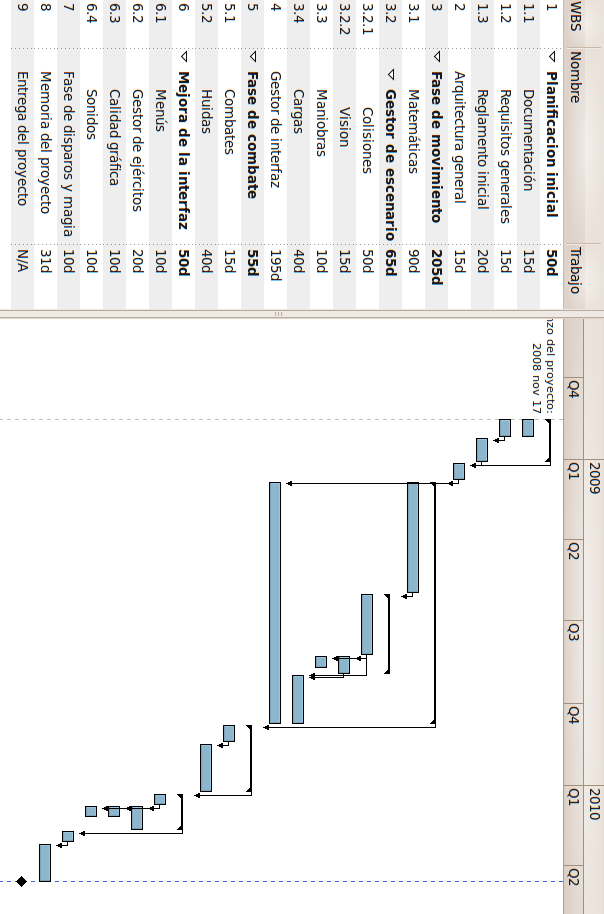
\includegraphics[scale=.5]{./imagenes/Gantt.png}
  \caption{Diagrama de Gantt del calendario del proyecto}
  \label{fig:gantt}
\end{figure}

\cleardoublepage

% Este archivo es parte de la memoria del proyecto fin de carrera
% de Aarón Bueno Villares. Protegida bajo la licencia GFDL.
%
% Para más información, la licencia completa viene incluida en el
% fichero fdl-1.3.tex

% Copyright (C) 2010 Aarón Bueno Villares

\section{Especificación de requisitos del sistema}
\label{sec:ers}

\subsection{Introducción}

Esta sección es una \emph{Especificación de Requisitos Software} (ERS) para el videojuego 2D de táctica militar basado en turnos, basado en reglamento y de corte medieval-fantástico \gomf. Esta especificación ha sido elaborada bajo el marco diseñado por el estándar \emph{IEEE Recommended Practice for Software Requirements Specification ANSI/IEEE 830 1998}.

\subsubsection{Propósito}
\label{sec:proposito}
El propósito de esta especificación es fundamentar las bases funcionales de \gomf. Está orientado tanto a los usuarios del sistema como a futuros desarrolladores. Esta especificación está sujeta a revisiones durante el ciclo de vida del producto, según las nuevas exigencias por parte de los usuarios finales, según posibles futuras inconsistencias o carencias, así como por los posibles caprichos de adición de funcionalidades por parte de el/los desarrollador/es.

\subsubsection{Alcance}
\label{sec:proposito}

\paragraph{\gomf}
\gom es un videojuego libre 2D de táctica militar por turnos y de corte fantástico-medieval (free fantasy turn-based tactics 2D-videowargame), de licencia GPL, y basado en reglamento (especificación estricta de todas las acciones posibles).

Está inspirado fuertemente en \textit{Warhammer Fantasy Battles} -de una alta vitalidad en el mercado-, un juego del mismo género, pero de mesa y con miniaturas, propiedad de la empresa inglesa Games Workshop.

\paragraph{Objetivos}
Este proyecto abarca la misión principal de desarrollar una alternativa digital, libre y gratuita, y si es posible, mejorada, del paradigma de juego cuyo máximo representante es \textit{Warhammer Fantasy Battles}.

No tiene como objetivo ser un juego de amplia difusión, ni con pretensiones de seducir a cualquier usuario potencial. Sus pretensiones van mas bien encaminadas a satisfacer las necesidades de jugadores que ya conocen dicho paradigma o para entusiastas de la táctica en general. Lo mas probable es que, para un jugador medio, el juego le parezca de lo mas artificial.

\paragraph{\emph{¿Qué hace y qué no hace el producto?}}
Esta pregunta se responde de la siguiente manera:
\begin{enumerate}
\item \gom no es un juego de estrategia, es un juego táctico.

La diferencia entre la táctica y la estrategia es difusa. La estrategia hace referencia a un propósito general, y la táctica al método para un fin específico. Estrategia es organizar una campaña militar en el lejano oriente. Táctica es un conjunto de movimientos específicos para ganar una batalla concreta, en la vida de dicha campaña. \gom se adentra en la segunda categoría.
 
\item \gom no es un juego de rol.

En los juegos de rol, el juego se organiza entorno a un personaje o conjunto reducido de personajes, que tienen una personalidad, un propósito y unas características. Mediante un conjunto de atributos, se modela toda la cosmovisión del/los personaje/s.

En \gomf, cada partida es independiente, y, aunque los distintos efectivos de cada unidad tengan atributos específicos que la modelan, la experiencia y posibles mejoras del usuario no tendrán efecto ninguno en el juego. \gom no distinguirá si un usuario es novato o un experto comandante, y la ejecución de una partida no tendrá efectos en la ejecución de partidas futuras, ni dependerá del éxito en partidas anteriores.

\item \gom no es un juego de tablero.

Un juego de tablero está basado en fichas que se desplazan sobre una
superficie organizada en casillas. \gomf, sin embargo, está mas bien un juego basado en elementos (unidades y efectivos) que pueden posicionarse en cualquier lugar de la ``mesa de juego''. Esto significa que los movimientos son completamente libres, y no están restringidos a movimientos en cantidades discretas, ni a posicionamiento en casillas.

\textit{Fantasy Wars} es el juego mas similar que he podido encontrar a \gom, pero está basado en un tablero tipo colmena (casillas hexagonales), y el jugador de ese modo ve limitada sus posibilidades de movimiento.

\end{enumerate}

\subsubsection{Visión general}
Esta ERS está organizada en tres subsecciones, a saber:
\begin{itemize}
\item  \textit{Introducción}: Es la subsección que en este momento
  estás leyendo. Explica qué es el producto y las directrices generales del documento.
\item \textit{Requisitos generales}: Se da una visión global del
  contexto funcional del producto: hardware y software implicado, así
  como la funcionalidad de mas alto nivel.
\item \textit{Requisitos específicos}. Se muestran, en concreto, cada una de las funcionalidades implicadas en el sistema.  
\end{itemize}

\subsection{Requisitos generales}
\subsubsection{Perspectiva del producto}
\begin{itemize}
\item \gom no pertenece a ningún producto mayor ni es parte de ningún otro software.
\end{itemize}

\subsubsection{Funciones del juego}
\begin{itemize}
\item La función principal del juego es permitir el enfrentamiento entre dos ejércitos, cada uno comandado por un usuario humano, según el reglamento de \gomf.
\item El usuario podrá crear su propio ejército.
\end{itemize}

\subsubsection{Características de los usuarios}
\begin{itemize}
\item Los usuarios que comanden cada ejército en una batalla deberán estar presentes en la misma máquina en la que se ejecute el juego.

\item Una vez los usuarios conozcan superficialmente el reglamento (las reglas mas generales), no tendrán problemas en habituarse velozmente y de forma intuitiva al uso del juego.
\end{itemize}

\subsubsection{Restricciones}
\begin{itemize}
\item El software tendrá una licencia libre, y en concreto, correrá bajo los derechos recogidos por la licencia GPL (GNU Public License).
\item Toda biblioteca usada para la implementación de este proyecto deberá ser multiplataforma.
\end{itemize}

\subsubsection{Suposiciones y dependencias}
Se asume que todos los requisitos descritos en esta especificación son consistentes e inmutables para la versión actual del producto. Todo posible cambio o modificación futura generará indefectiblemente una nueva versión del producto. La versión del producto actual es la 1, y será, asimismo, la versión de esta especificación así como la versión del documento de diseño generado a partir de esta especificación.

Si se propone una ampliación de los requisitos del sistema, sin modificar los existentes, se generará indefectiblemente una nueva subversión del producto. La subversión actual es la 1.0, y será, asimismo, la subversión de esta especificación así como la subversión del documento de diseño generado a partir de esta especificación.

\subsection{Requisitos específicos}

\subsubsection{Requisitos de interfaz externa}

\requisito{requisitos/interfazusuario}
\requisito{requisitos/interfazhardware}
\requisito{requisitos/velocidadreaccion}
\requisito{requisitos/resolucionpantalla}
\requisito{requisitos/sonido}

\subsubsection{Requisitos funcionales}

\requisito{requisitos/comenzarbatalla}
\requisito{requisitos/crearejercito}
\requisito{requisitos/editarejercito}
\requisito{requisitos/salir}
\requisito{requisitos/modificarejercito}
\requisito{requisitos/elegirraza}
\requisito{requisitos/informaciontarea}
\requisito{requisitos/ejecutartarea}

\subsubsection{Requisitos de rendimiento}

\requisito{requisitos/tiempo}
\requisito{requisitos/memoria}

\subsubsection{Restricciones de diseño}

\requisito{requisitos/enfoqueOO}
\requisito{requisitos/estandardiseno}

\subsubsection{Atributos del sistema software}

\requisito{requisitos/completitud}
\requisito{requisitos/documentacion}
\requisito{requisitos/escalabilidad}
\requisito{requisitos/portabilidad}
\requisito{requisitos/robustez}
\requisito{requisitos/usabilidad}
\requisito{requisitos/licencia}

\subsubsection{Otros requisitos}

\requisito{requisitos/implementacion}
\requisito{requisitos/librerias}

\cleardoublepage

% Este archivo es parte de la memoria del proyecto fin de carrera
% de Aarón Bueno Villares. Protegida bajo la licencia GFDL.
%
% Para más información, la licencia completa viene incluida en el
% fichero fdl-1.3.tex

% Copyright (C) 2010 Aarón Bueno Villares

\section{Análisis y diseño del sistema}
\label{sec:diseno}

\subsection{Confección del reglamento}
Se pueden forjar muchas preguntas sobre qué va a tener un juego de
táctica militar. A su vez, se pueden forjar otras tantas acerca de qué
va a tener un juego de corte fantástico. En suma, hay una gran
diversidad de preguntas por contestar.

Aquí se muestra un grupo de ellas:
\begin{itemize}
\item \emph{¿Qué razas estarán disponibles?}
\item \emph{¿Qué elementos de una batalla real vamos a considerar?}
\item \emph{¿Sobre qué tipo de terrenos se va a combatir?}
\item \emph{¿Cómo se organizará cada ejército?}
\item \emph{¿Con cuántos elementos fantásticos se trabajará?}
\item \emph{¿Qué tiempo de batalla real representará cada turno de
    juego?}
\item \emph{¿Cómo representaremos la escena y con qué elementos de
    escenografía contaremos?}
\item \emph{¿Cómo modelaremos las capacidades de cada ``soldado''?}
\end{itemize}

Todas estas preguntas han necesitado responderse a fin de confeccionar
un reglamento consistente. Por otro lado, si bien es cierto que
\gomf, por el simple hecho de ser un juego basado en turnos, no
constituye una simulación real de ninguna batalla campal, sí que es una
buena aproximación esquemática de su contenido (podría aplicarse aquí el
calificativo de simulación conceptual).

Este factor hace falta tenerse en cuenta para crear un reglamento
coherente. Intentar modelar aspectos que son demasiado característicos
del \emph{tiempo real} en una serie de turnos puede resultar
artificial. Así, no deberíamos sentirnos incómodos si decidimos
ordenar en un mismo turno acciones que ocurren
simultáneamente. Es el precio a pagar si queremos diseñar un juego
basado en turnos.

Por último, en una batalla ocurre una gran multitud de cosas. No
podemos, \emph{a priori}, considerarlas todas. Por ello, también
veremos adecuado forjarnos ciertas fronteras funcionales; por
cuestiones de viabilidad.

La muestra final de este reglamento se encuentra en el anexo
\ref{reglamento}.

\subsection{Arquitectura general del sistema}
Como hemos venido mencionando, nuestro juego está basado en un
reglamento. Existirá, por tanto, una entidad encargada de gestionar
dicho reglamento. Ésta será la parte lógica de nuestro sistema. Por
otro, es necesario una interacción con el usuario donde poder elegir
las acciones que, en cada momento de la partida, ofrece \gomf.

A fin de organizar el diseño en la clásica arquitectura de capa de
presentación y capa de dominio, hemos considerado, primeramente, dos
clases principales: \emph{gestor de interfaz} y \emph{gestor de
  reglas}.

Está claro que la capa de dominio es representada completamente por
el reglamento, comprendiendo la capa de presentación su interfaz de
interacción con el usuario. El
\emph{gestor de reglas} es el resposanble pues, de la capa de dominio,
y el \emph{gestor de interfaz} de la capa de presentación.

El \emph{gestor de interfaz}, a parte de disponer al usuario del menú
principal del juego y la confección de ejércitos, se encarga, una vez
dentro de una batalla, de mostrar al usuario todas las acciones
disponibles, responder a las peticiones del usuario y mostrar los
cambios producidos por éstas. También gestiona el sonido del juego.

Y por último, para hacer efectiva esa interacción entre ambas clases,
dispondremos de otras dos, la clase \emph{estado}, que encapsulará la
información usada como \emph{testigos} pasados en los cambios
producidos dentro de cada capa, y la clase \emph{juego}, la de más
alta jerarquía en el juego, que se encargará de encapsular a los
gestores.

\begin{figure}[h]
\centering
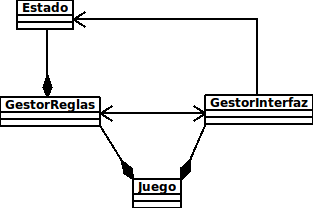
\includegraphics[scale=.8]{./imagenes/DiagramaJuego.png}
\label{fig:arqgen}
\caption{Arquitectura general del sistema (UML)}
\end{figure}

El proceso global y principal del juego es el siguiente:

\begin{enumerate}
\item Al lanzar el juego, la clase \emph{juego} inicializa al gestor
  de interfaz y lanza su menú.
\item Los deseos del usuario (la opción elegida del menú) se devuelven
  a la clase \emph{juego} para que actúe en consecuencia.
\item Si se eligió comenzar una batalla, los usuarios eligen los
  dos ejércitos combatientes y la clase \emph{juego}, acto seguido,
  inicializa al \emph{gestor de reglas} (acto que da comienzo a la
  partida).
\item El \emph{gestor de reglas} entrega al \emph{gestor de interfaz}
  el estado inicial del juego.
\item Con esa información el gestor de interfaz imprime
la situación actual de la batalla y ofrece al usuario todas las
acciones disponibles para continuar jugando, información que se
obtiene también del \emph{estado}.
\item Si el usuario realiza alguna acción, la interfaz envía esa
  información al \emph{gestor de reglas}.
\item El gestor de reglas modifica con esa información
  el estado interno del juego.
\item Se repite el proceso hasta que el gestor de interfaz
  reciba un estado final.
\item Tras esto, se muestra el resultado de la partida y se vuelve al
  menú principal del juego.
\end{enumerate}

\subsection{Capa de dominio}
\subsubsection{Estado y acciones}
El reglamento indica que existen seis turnos para cada jugador, y
cada turno se divide en dos fases: movimiento y combate. Por último,
cada fase se divide en ciertas subfases, donde se pueden realizar
ciertas acciones.

Consideraremos que una \emph{acción} posee un nombre o etiqueta, que
llamaremos \emph{tarea}, mas toda la información necesaria para que esa
acción pueda ejecutarse. Por ello, tendremos una enumeración que
contendrá la lista de etiquetas de las acciones disponibles, y una
clase concreta para cada acción, cuyos atributos serán los datos
necesarios para que dicha acción pueda realizarse. Por ejemplo, para
la acción \emph{declaración de carga}, su único atributo será la
unidad objetivo (luego el gestor de reglas evaluará si esa carga será
efectiva o fállida, pero con esa información la acción queda
completamente definida).

Evidentemente, existe cierto comportamiento e información genérica que
comparten todas las acciones concretas, como la fase sobre la que está
definida, o la tarea que la etiqueta. Por ello, existirá una clase
base llamada acción, y una clase heredada por cada acción posible en
\gomf. A su vez, cada clase heredada (cada acción concreta) añadirá el
conjunto de atributos adicionales necesarios para su propia
definición.

\begin{figure}[h]
\centering
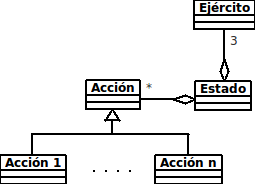
\includegraphics[scale=.8]{./imagenes/Estado.png}
\label{fig:estado}
\caption{Clase estado y clase acción (UML)}
\end{figure}

Con respecto al estado, contendrá toda la información necesaria y
relativa a un estado concreto de la partida: jugador actual, turno
actual, así como la fase y subfase actual del turno del jugador en
curso.

Pero esto solo define a un estado, quizás, desde el punto de vista del
reglamento. Desde el punto de vista de nuestra jerarquía de clases, un
estado concreto de juego es definido por mas aspectos.

La interfaz tiene como su única fuente de información el tipo estado,
y como se ha de imprimir la situación actual de los ejércitos
involucrados (los dos ejércitos combatientes, y el ejército GAIA), el
tipo estado también debe proveerlo.

Por último, aunque la interfaz conozca todas las acciones existentes,
no necesariamente debe conocer cuando sí y cuando no están
disponibles cada una de ellas. El \emph{gestor de reglas} es la
entidad encargada de mantener actualizada esta información en el
estado a medida que transcurre la partida, para que luego la interfaz
tenga acceso a él y disponga al usuario la disponibilidad funcional
actual correcta.
%%TODO: Gráfico de estado con ejército y lista de acciones tareas.

\subsubsection{Ejército y unidades}
El tipo unidad es el tipo básico sobre el cual gira \gomf. Existen
solamente dos razas distintas, y cada raza tiene en concreto nueve
unidades distintas\footnote{El hecho de que sean nueve no es por
  ninguna razón concreta, sencillamente es el límite que la
  imaginación me impone.}.

Toda modificación de la posición de una unidad, su número de
efectivos, y toda información referida a ella está poseida en la
propia clase, como era de esperar. A su vez, la clase ejército es,
básicamente, la encapsulación de una serie de unidades que pertenecen
al mismo bando, y fundamentalmente no contiene ninguna información
adicional.

Existirá, por tanto, un tipo heredado particular para cada una de las
razas, y un tipo heredado particular para cada uno de las unidades de
cada raza.

\begin{figure}[h]
\centering
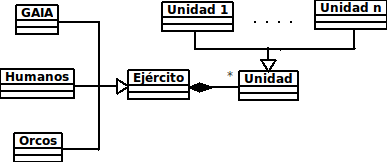
\includegraphics[scale=.8]{./imagenes/Ejercitos.png}
\label{fig:ejercitos}
\caption{Clase ejército y clase unidad (UML)}
\end{figure}

\paragraph{GAIA}
Usualmente, en muchos juegos de estrategía, se cuenta con un ejército
especial llamado ``GAIA'' que es transparente al jugador, y es usado
por la aplicación para gestionar el comportamiento general del
escenario de juego.

Esto se hace evidente en algunos juegos que tienen un editor de
escenarios. Por ejemplo, en el juego \emph{Tzar}, un juego de
estrategía de la compañia \emph{FX}, se disponía de distintos menús,
uno para cada equipo de la partida que estuvieses diseñando, que te
permitía colocar en el mapa los elementos disponibles del mismo:
edificios, unidades, objetos, etc. Y, a su vez, disponía de un
``equipo'' adicional llamado GAIA, y con él, se podían añadir
montañas, bosques, animales, minas de recursos, etc.

En \gom hemos adoptado la misma convención, y para los elementos de
escenografía hemos utilizado la estructura general de la clase
\emph{ejército} para crear un nuevo ejército llamado \emph{GAIA}.

La ventaja de usar GAIA como ejército es que los elementos de
escenografía son tomadas entonces como unidades, lo que nos permite hacer
un trato directo de estos elementos para realizar los cálculos sobre
visibilidad de las unidades o las capacidades de movimiento de las
mismas, ya que dichos elementos escenográficos son tratados como
elementos impasables y además, ocultan la visibilidad del mismo modo que
cualquier otra unidad.

\subsubsection{Gestor de reglas}
El gestor de reglas, mas que una clase, es una entidad compuesta por
una serie de clases que gestionan las acciones ejecutadas y
que mantiene el control del reglamento.

Estrictamente hablando, el gestor de reglas es una única clase muy
general que solo ejecuta una serie de acciones básicas. El núcleo de
la funcionalidad recae sobre otras clases concretas específicas para
cada fase.

\begin{figure}[h]
\centering
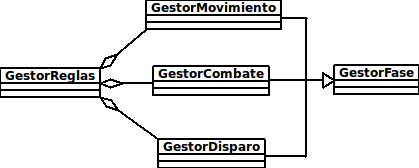
\includegraphics[scale=.8]{./imagenes/Reglas.png}
\label{fig:reglas}
\caption{Gestor de reglas (UML)}
\end{figure}

Sin embargo, podemos usar indistintamente el término entidad o clase
\emph{gestor de reglas} para referirnos a la entidad concreta ya que
dicha clase funciona como un API de toda la entidad. De este modo,
toda acción recibida se envía al gestor de reglas, y si hace falta
transmitir dicha información a una clase de fase específica, el gestor
de reglas se encargara de ello, y nunca la interfaz, ni ninguna clase
intermediaria o auxiliar tendrá acceso a ellas.

El proceso es el siguiente:
\begin{enumerate}
\item El gestor de reglas recibe una nueva acción.
\item Si la acción es una acción general\footnote{Las acciones se
    jerarquizan en tres clases: acciones de movimiento, acciones de
    combate, y acciones generales. Las acciones generales son todas
    aquellas que no se pueden emarcar en ninguna de las dos
    anteriores, por ejemplo, la elección de una unidad o el comienzo
    de un nuevo turno.}, es gestionada directamente por el gestor.
\item Si no es una acción general, y es una acción de la misma fase
  que la actual, se pasa el control a dicha clase de fase, junto al
  estado actual y el gestor de escenario -de este modo, la fase
  correspondiente tiene todas las herramientas necesarias para
  evaluar y ejecutar la acción-.
\item Si no es una acción general, pero la fase a la que pertenece la
  acción no coincide con la fase en curso, no se produce ningún cambio
  en el estado de juego.
\end{enumerate}

En concreto, existirán tres gestores de fases, el \emph{gestor de
  movimiento}, el \emph{gestor de combate} y el \emph{gestor de
  disparo}, cada una encargada de gestionar el desarrollo de cada
fase. Como pasaba con el tipo acción, existe cierto comportamiento
genérico común de dichas clases de fase, así como por el trato dado
por el gestor de reglas. En definitiva, dichas clases serán herencias
concretas de una clase base llamada \emph{gestor de
  fase}\footnote{Este \emph{convenio} permite, además, 
  aumentar la escalabilidad del producto, ya que se automatiza en
  parte la inclusión de nuevas fases futuras, como puede ser el
  disparo o la magia.} \footnote{La relación incluida en el gráfico,
  entre el gestor de movimiento y el de combate, existe debido a que
  es necesaria cierta comunicación entre ambos gestores cuando se
  realizan nuevas cargas, que implican nuevos combates -o cambios
  sobre los combates existentes en la fase de movimiento-.}

\subsubsection{Gestor de escenario y matemáticas}
Esta clase es una clase excepcional que no es intermediaria entre la
entidad de reglas y de interfaz, pero que son requeridas por igual por
ambas, y en concreto, por la clase \emph{GestorMovimiento} y
\emph{GestorInterfaz}.

Es aquella que provee toda la funcionalidad necesaria para
realizar acciones que dependen de la situacion de una unidad respecto
al resto de unidades, es decir, la única que trabaja considerando al
conjunto de unidades y el espacio -escenario- donde éstas residen.

Por ejemplo, en esta clase se calcula si una unidad ve
\refreg{visibilidad} a otra unidad, ya que dicha visibilidad depende
del resto de unidades presentes en el escenario. Si existen unidades
en el camino de una unidad a otra, o la unidad objetivo está en alguna
posición fuera del rango de visibilidad de la primera, la función 
miembro correspondiente de la clase devolverá si es cierto o no que
dicha visibilidad exista. Ocurre lo propio en el movimiento de carga,
el movimiento de huida, o la distancia máxima de movimiento o
pivotaje.

Por último, existe un \emph{módulo}\footnote{Lo notamos como módulo
  porque no es una clase única con una serie de funciones miembro,
  sino una serie de estructura y funciones independientes -aunque
  interrelacionadas-.}, llamado matemáticas, que provee una serie de
estructuras y funciones, principalmente geométricas -idoneas sobre
todo para la naturaleza de los cálculos realizados por el gestor de
escenarios-, que son las únicas que necesitamos para estos
cálculos.

\begin{figure}[h]
\centering
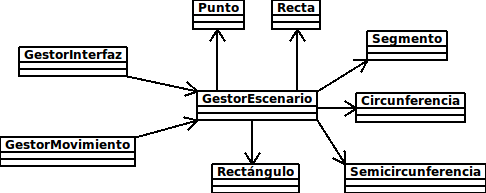
\includegraphics[scale=.8]{./imagenes/Escenario.png}
\label{fig:escenario}
\caption{Gestor de escenario y módulo matemático (UML)}
\end{figure}

\subsection{Capa de presentación}
\subsubsection{Gestor de interfaz}
Al igual que pasaba con el gestor de reglas, esta clase funciona como
API para toda la entidad de interfaz, compuesta por una serie más
compleja de clases.

El comportamiento del gestor de interfaz se puede dividir en tres
\emph{partes} fundamentales:
\begin{itemize}
\item Control de menú.
\item Gestión de ejércitos.
\item Interfaz de batalla.
\end{itemize}

El control del menú es controlado directamente por el gestor de
interfaz. La gestión de los ejércitos (creación y edición de
ejércitos), está completamente controlada por la clase \emph{gestor de
  ejércitos}. Y por último, la interfaz de batalla es controlada por
el propio gestor de interfaz pero esta vez ayudada por el \emph{gestor
  de iconos} para la gestión, muestra y captura de iconos y captura
(que no procesamiento) de acciones elegidas por el usuario (y como ya
hemos mencionado, por el \emph{gestor de escenario} para realizar los
cálculos involucrados).

\begin{figure}[h]
\centering
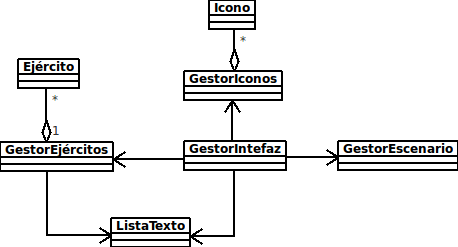
\includegraphics[scale=.8]{./imagenes/Interfaz.png}
\label{fig:interfaz}
\caption{Gestor de intefaz (UML)}
\end{figure}

\subsubsection{Lista de textos}
Es una clase auxiliar usada por el control de menú y la gestión de
ejércitos que provee una especie de \emph{motor} para trabajar con
listas de elementos textuales que te permiten seleccionar, etiquetar,
añadir y eliminar los distintos ítems que pueden formar las listas.

Por ejemplo, si el usuario hace click en un item de la lista, se
imprime una imagen sobre dicho item para
indicar que ha sido seleccionado (dicha imagen será pasada por el
usuario en la contrucción de la lista). Si la lista contiene mas items
que los permitidos para visualizar a la vez, se imprime un scroll para
poder desplazarte por la lista, o si se indica que se desea etiquetar
un item, se desplaza el item para dejar hueco a la etiqueta, de modo
que el conjunto quede nuevamente centrado.

Esta clase resulta muy útil para gestionar, sobre todo, el menú
contextual de la edición y creación de ejércitos, usado para imprimir
la lista de unidades disponibles de una raza dada, la lista de razas
disponibles, el sumario de la configuración actual del ejército, o la
lista de ejércitos creados.

\subsubsection{Gestor de ejércitos}
Es la clase encargada de controlar y mantener, mediante menús para el
usuario, el conjunto de ejércitos existentes, eliminarlos o crear
ejércitos nuevos, así como 
modificarlos y elegirlos cuando comienza una batalla. Comprueba,
además, que los ejércitos creados o modificados sean correctos (que no
existan unidades fuera de la zona de despliegue o \emph{pisándose} en
dicha zona de despliegue), o que los ejércitos elegidos de un combate
estén equilibrados en puntos, tal y como indica el reglamento de
\gomf.

Debido a la simplicidad de un ejército, la información de los
ejércitos existentes es guardada en ficheros de texto plano
simples. En ellos se guarda la lista completa de ejércitos, y el
contenido de cada uno de ellos.

\subsubsection{Gestor de iconos}
Un icono es un elemento contextual que identifica a una acción
concreta. Así, el gestor de iconos imprime la secuencia de iconos
correspondientes a las acciones disponibles\footnote{En realidad,
  imprime las acciones activas mas las disponibles.}, además de
proveer una descripción de cada icono, como ayuda contextual para el
usuario.

La forma de actuar del gestor de iconos es la siguiente:
\begin{enumerate}
\item Se obtiene, a partir del estado, la lista de acciones
  activas.
\item Se imprimen todos los iconos, distinguiéndose los que están
  disponibles de los que no, en zonas separadas de la zona de iconos.
\item Si el ratón se situa sobre la posición actual del icono, se
  devuelve la descripción de dicho icono.
\item Si el ratón pulsa sobre el icono, se devuelve su acción
  correspondiente, y el gestor de interfaz se encarga de pedir al
  usuario la información necesaria para completar la acción.
\end{enumerate}

Un objeto icono es el elemento sobre el que el \emph{gestor de iconos}
actua. Un icono contiene la acción a la que está asociada, mas la
imagen que la identifica, así como la posición concreta adquirida
durante la vida de la batalla.
\cleardoublepage

% Este archivo es parte de la memoria del proyecto fin de carrera
% de Aarón Bueno Villares. Protegida bajo la licencia GFDL.
%
% Para más información, la licencia completa viene incluida en el
% fichero fdl-1.3.tex

% Copyright (C) 2010 Aarón Bueno Villares

\section{Principales problemas de implementación}
\label{sec:implementacion}

En este capítulo se abordarán algunas cuestiones de implementación
que, por su dificultad (e importancia asociada), merecen una atención
especial, o al menos, el deseo del autor de merecer una atención
especial.

Nos estamos refiriendo a problemas de implementación
funcional, es decir, de implementación a la hora de establecer un
cómputo que calcule a una función que resuelva un problema, y no a problemas de implementación
estructural, es decir, encargados de organizar los datos con los que
se trabajará y de asignar responsabilidades. Estos últimos ya han sido comentados en el capítulo de
análisis y diseño.

El asunto que forma base de \gom a nivel de reglas, es su
geometría. En \gom todo se reduce a figuras geométricas: las unidades
son rectángulos, al igual que el escenario; sus pivotajes y la visión se reducen a
problemas dentro y entre circunferencias, y, como veremos, los problemas mas importantes
del juego se reducen todos también a problemas geométricos.

Particularmente, estos problemas, como se ya se ha indicado, se resuelven
con la clase \emph{Gestor de escenario}, pues estos problemas
están ligados a la relación entre las distintas unidades presentes en
el escenario.

Tendremos una sección dedicada a los problemas que, para mí, han
resultado mas singulares sobre todo por su transfondo matemático en la
resolución. Existen otros
problemas que tampoco han sido fáciles de resolver a lo largo del
código. Por ejemplo, la
implementación de la clase \emph{Lista texto} o la resolución de los
combates en \emph{Gestor de combates}, debido a su ``\emph{desorden}''
conceptual (una amalgama de datos interrelacionados que hay que
manejar a la vez), son un ejemplo de aquellos problemas para nada
inmediatos a los que me he tenido que enfrentar. Pero la naturaleza de
estos problemas es fundamentalmente discreta, y encontrar su correcta
solución solo merece la observación atenta de sus partes sin la
necesidad de recurrir al ingenio ni a herramientas conceptules
externas.

En su lado extremo, tenemos los problemas como la caraterización de la
visión o el pivotaje máximo de una unidad, cuya resolución no es
\emph{a priori} intuitiva (ni \emph{a posteriori} tampoco).

\subsection{Pertenencia de un punto a una figura}
Para encontrar si el usuario ha hecho click en un icono, ha
seleccionado una unidad, si la esquina superior derecha de una unidad
está dentro del área de pivotaje de otra que desea moverse, o si la
intersección de dos rectas pertenece a un segmento, se hace necesario
disponer de dicha función para todas las estructuras geométricas a las
que sean aplicables (es decir, a todas).

Podemos encontrarnos con que necesitamos saber si un punto pertenece a una
recta, a una semicircunferencia o a un rectángulo con cualquier
orientación, por ejemplo. Para los casos en los que la figura
geométrica es descrita por una ecuación, su resolución es sencilla:
basta con ver si se verifica la ecuación de la figura sustituyendo en
ella la coordenada $x$ e $y$ del punto. Éste es el caso de la
pertenencia de un punto a una recta o a una circunferencia.

En el caso de la semicircunferencia, se traza una recta desde su
origen hasta el punto en cuestión, y si el ángulo de esta recta está
comprendida entre la de las dos rectas que definen a los extremos de
la semicircunferencia, y la longitud de dicha recta es menor a su
radio, el punto pertenece a la semicircunferencia, por lo tanto su
resolución también es bastante simple.

Pero para el caso de un rectángulo, que tampoco tiene ninguna ecuación
que lo defina, el problema se complica.

Podriamos pensar en trazar una recta desde cualquiera de sus vértices
hasta el punto en cuestión, he intentar ver si dicho segmento pertenece
al área del rectángulo, pero eso sencillamente es otra versión quizás mas
general del problema de la pertenencia de un punto a la
figura. También se podrían trazar cuatro segmentos, uno desde cada
vértice, y caracterizar los ángulos de cada pareja de segmentos. O la
suma de sus longitudes. Pero la solución que hemos adoptado es
computacionalmente mas sencilla, y esta basada en construir triángulos
alrededor de un punto.

\subsubsection{Orientación de un triángulo}
Imaginemos un triángulo $ABC$. Diremos que este triángulo tiene
orientación positiva si, al leer sus puntos en el plano en el orden
dado, se consigue una dirección horaria, y en caso contrario, su
orientación será negativa.

\begin{center}
\begin{tabular}{cc}
\begin{tikzpicture}[scale=2, decoration = {
    markings,
    mark=at position .10 with {\arrow[red, line width = 1.5pt]{>};} ,
    mark=at position .43 with {\arrow[red, line width = 1.5pt]{>}} ,
    mark=at position .76 with {\arrow[red, line width = 1.5pt]{>};} }
  ]
  \draw[gray,postaction={decorate}] (0,0) circle (1cm);
  \draw[thick,blue] (120:1cm) -- (240:1cm) -- (360:1cm) -- cycle;
  \filldraw[green] (120:1cm) circle(1pt);
  \filldraw[green] (240:1cm) circle(1pt);
  \filldraw[green] (360:1cm) circle(1pt);
  \draw (120:1.2cm) node[fill=white] {$A$};
  \draw (240:1.2cm) node[fill=white] {$B$};
  \draw (360:1.2cm) node[fill=white] {$C$};
\end{tikzpicture}
&
\begin{tikzpicture}[scale=2, decoration = {
    markings,
    mark=at position .10 with {\arrow[red, line width = 1.5pt]{<};} ,
    mark=at position .43 with {\arrow[red, line width = 1.5pt]{<}} ,
    mark=at position .76 with {\arrow[red, line width = 1.5pt]{<};} }
  ]
  \draw[gray,postaction={decorate}] (0,0) circle (1cm);
  \draw[thick, blue] (180:1cm) -- (300:1cm) -- (60:1cm) -- cycle;
  \filldraw[green] (180:1cm) circle(1pt);
  \filldraw[green] (300:1cm) circle(1pt);
  \filldraw[green] (60:1cm) circle(1pt);
  \draw (180:1.2cm) node[fill=white] {$A$};
  \draw (300:1.2cm) node[fill=white] {$C$};
  \draw (60:1.2cm) node[fill=white] {$B$};
\end{tikzpicture}
\end{tabular}
\end{center}

En este caso, vemos como la primera figura muestra una orientación
negativa (según nuestro convenio adoptado), por ir en sentido
antihorario, mientras que la segunda figura muestra una orientación
positiva al ir a favor de las agujas del reloj, según la lectura de
los vértices $A$, $B$ y $C$.

El motivo está muy relacionado con la regla que nos enseñaban en el
colegio de la mano derecha o del sacacorchos, aunque nosotros hemos
invertido su polaridad (por comodidades en la implementación). Si
giramos la mano en la
misma dirección que la que nos dicta el orden de lectura de los
vértices, si su sentido es anti-horario, será como sacar un
sacacorchos. Y lo opuesto si su sentido es horario.

Esta es consecuencia directa del producto vectorial de dos vectores en
un plano. Imaginemos que, en un espacio tridimensional, tenemos dos
vectores $\vec{u}$ y $\vec{v}$ en el plano $z=0$, es decir, que
$\vec{u} = ( u_x, u_y, 0)$ y $\vec{v} = (v_x, v_y, 0)$.

Si desarrollamos matemáticamente el producto vectorial en nuestras
condiciones, y tomando $\vec{u} = B - A$ y $\vec{v} = C - A$ para caracterizar al
triángulo $ABC$, tenemos:

\[ \vec{u} \times \vec{v} = 
  \begin{vmatrix}u_y & 0 \\v_y & 0 \\\end{vmatrix} \vec{i}
  - \begin{vmatrix}u_x & 0 \\v_x & 0 \\\end{vmatrix} \vec{j}
  + \begin{vmatrix}u_x & u_y \\v_x & v_y \\\end{vmatrix} \vec{k}
 = (u_xv_y - u_yv_x)\vec{k} = p\vec{k} \]

Como $\vec{k}$ es el vector de la base ortonormal correspondiente al
eje $z$, cuando $p>0$, significará que el producto vectorial crece por
el eje $z$, es decir, que la orientación del triángulo es antihoraria,
y bajo nuestro convenio, su orientación será negativa. En caso
contrario, será positiva.

Mas esquemáticamente:

\[orientacion(ABS) = \left\{
  \begin{array}{lc}
    positiva & |\vec{u}\times\vec{v}| \leq 0\\
    negativa & |\vec{u}\times\vec{v}| > 0\\
\end{array} \right. \]

Cuando el módulo del producto vectorial es 0, significa que los tres
puntos se encuentran en una misma linea recta. Consideraremos en este
caso que su orientación también es positiva dado que usaremos este resultado para
verificar que un punto pertenezca a la figura.

\subsubsection{Pertenencia de un punto a un rectángulo}
Ahora que sabemos caracterizar la orientación de un triángulo respecto
a sus vértices, veremos como podemos aplicar estos resultados al
problema de la pertenencia de un punto en un rectángulo (y en general,
en cualquier poliedro).

\begin{minipage}[h]{0.4\columnwidth}
\centering
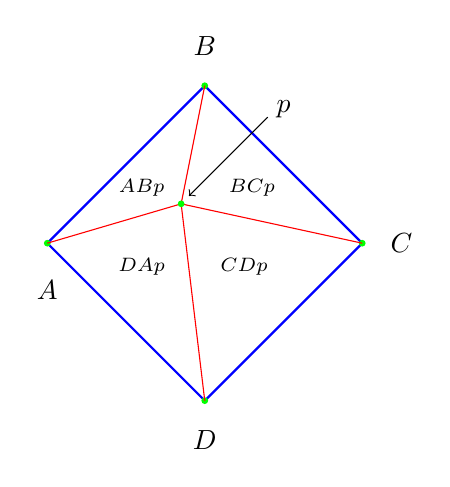
\begin{tikzpicture}
\draw[thick,blue] (0,0) -- (2,2) -- (4,0) -- (2,-2) -- cycle;

\filldraw[green] (0,0) circle(1pt);
\filldraw[green] (2,2) circle(1pt);
\filldraw[green] (4,0) circle(1pt);
\filldraw[green] (2,-2) circle(1pt);

\draw (0,-0.6) node {$A$};
\draw (2,2.5) node {$B$};
\draw (4.5,0) node {$C$};
\draw (2,-2.5) node {$D$};

\draw (3,1.7) node[fill=white] {$p$};
\draw[->] (2.8,1.6) -- (1.8,0.6);

\draw [red] (0,0) -- (1.7,0.5);
\draw [red] (2,2) -- (1.7,0.5);
\draw [red] (4,0) -- (1.7,0.5);
\draw [red] (2,-2) -- (1.7,0.5);

\filldraw[green] (1.7,0.5) circle(1pt);

\draw (1.2,0.7) node {$\scriptstyle ABp$};
\draw (2.6,0.7) node {$\scriptstyle BCp$};
\draw (2.5,-0.3) node {$\scriptstyle CDp$};
\draw (1.2,-0.3) node {$\scriptstyle DAp$};
\end{tikzpicture}
\end{minipage}
\begin{minipage}[h]{0.6\columnwidth}
La idea general es la siguiente: si un punto pertenece a una figura, y
construimos distintos triángulos con ese punto como uno de sus
vértices, la orientación de todos estos triángulos formados debe ser
la misma.

Por ejemplo en la figura de la izquierda, vemos como es importante el
orden en que se escogen los vértices de los triángulo. Deben escogerse
de modo que, si el punto efectivamente pertenece a la figura, todas
las orientaciones sean la misma, y en concreto, positiva. Para ello,
siempre hemos construido los triángulos en sentido horario y con el
punto $p$ como tercer vértice.
\end{minipage}

 Si por
ejemplo el segundo triángulo fuera $CBp$ en vez de $BCp$, el módulo de
su producto vectorial sería positivo, y por lo tanto su orientación
negativa, y nuestro método no funcionaría: el resto de triángulos
tendría una orientación positiva, sus orientaciones serían distintas,
y se nos indicaría que el punto no pertenece a la figura, lo cual es
falso.

Aquí se hace evidente por qué decidimos dar una orientación positiva
al caso $|\vec{u}\times\vec{v}| = 0$. En este caso, en nuestra
construcción de la figura, implicaría que el punto $p$ pertenece a una
arista (la correspondiente al triángulo construido actualmente) o
incluso a un vértice, y un punto que pertenece a una arista o un
vértice de la figura pertenece a la propia figura.

Es fácil ver como este método es aplicable directamente a cualquier
problema de pertenencia de un punto a un poliedro, su cálculo es muy
sencillo y computacionalmente es muy óptimo, pues su coste asintótico
es lineal respecto al número de vértices de la figura (dado que para
$n$ vértices, hay que construir $n$ triángulos y calcular el sentido
de cada uno de ellos).

Este problema me resulta importante por ser el primer problema
geométrico con el que me tuve que enfrentar en el juego, preparando
terreno para lo que vendría a continuación. Tras esto, se creó un
conjunto de estructuras y funciones que resolvían muchos otros
problemas geométricos necesarios, algunos sencillos de crear y otros
necesitando calma y tiempo para encontrar una solución correcta y
potente; cabe mencionar aquí el trato de rectas (caracterizadas como
hiperplanos) y el trato con circunferencias (sobre todo sobre la
intersección de circunferencias).

\subsection{Capacidades de movimiento actual}
El mundo de la intersección vino a tomar forma viva en este
problema. Tenemos tres casos del mismo: movimiento \emph{rect} máximo,
pivotaje derecho máximo, y pivotaje izquierdo máximo.

Tales problemas vienen delimitados por una máxima: no podrás acercarte
a menos de 10 unidades de terreno (véase reglamento) de otra unidad, sea amiga o
enemiga, y esto añade una dificultad interesante en el caso de los
pivotajes.

\subsubsection{Desplazamiento máximo}
En este problema se debe conseguir saber cual es la longitud máxima
que puede desplazarse una unidad en linea recta. Una unidad dispone de
un desplazamiento máximo de partida, y se ha de saber si existen
unidades en el camino que dificulten recorrer ese desplazamiento
máximo, teniendo en cuenta la distancia de respeto de 10 unidades de
terreno de juego entre unidades del mismo o distinto bando.

El problema se caracteriza de la siguiente forma: se construye un
rectángulo que tenga por ancho el frente de la unidad, y por alto, el
desplazamiento máximo de la unidad. Ahora se ha de ver qué unidades
enemigas tienen intersección con ese rectángulo (una unidad no es más
que otro rectángulo que caracteriza su ubicación), e ir calculando el
rectángulo libre de máxima altura a partir del rectángulo original.

Dos figuras pueden estar en posición una respecto a la otra de las
siguientes formas:
\begin{itemize}
\item Figuras disjuntas: cuando no tienen intersección.
\item Figuras contenidas: cuando su intersección es uno de los dos
  rectángulos.
\item Figuras cruzadas: cuando los vértices de su intersección no son
  vértices de ninguno de los dos rectángulos.
\item Figuras secantes: cuando su intersección contiene vértices
  de alguno de los dos rectángulos.
\end{itemize}

Esta taxonomía es importante por los siguientes motivos:
\begin{itemize}
\item Si buscamos vértices de otra figura, que pertenezcan a un
  dada, estoy encontrando figuras secantes y contenidas.
\item Si busco intersecciones de aristas, encuentro figuras secantes y cruzadas.
\item En caso contrario, las figuras son independientes.
\end{itemize}

Además, partimos del hecho de que la unidad de origen es una figura
\emph{bien colocada}. Con esto quiero decir que como partida la unidad
es disjunta a cualquier otra, y además, con 10 unidades de terreno de
separación, por lo tanto, el rectángulo de desplazamiento no estará
nunca contenida en ninguna otra figura, y nunca tendré que buscar que
sus vértices pertenezcan a las restantes.

\begin{minipage}[h]{0.4\columnwidth}
\centering
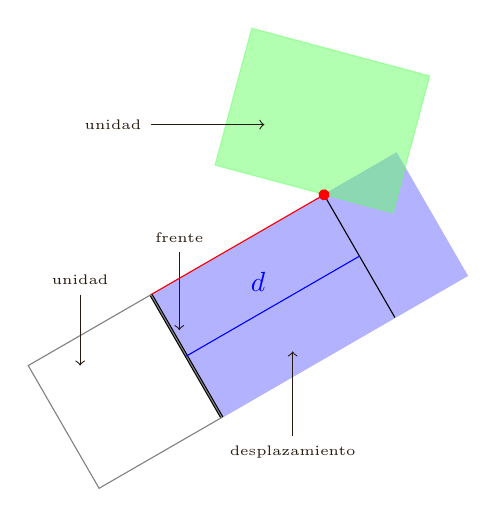
\begin{tikzpicture}[scale=1.8]
\filldraw[rotate=300,blue!30] (0,0) -- (1,0) -- (1,2) -- (0,2) --
cycle;
\filldraw[rotate=300,very thick] (0,0) -- (1,0);
\draw[brown!20!black,->] (.2,.3) node[above] {\tiny{frente}} -- (0.2,-.25);
\filldraw[rotate=345,opacity=.5, green!60] (0.2,1) -- (1.5,1) -- (1.5,2) -- (0.2,2) -- cycle;
\draw[rotate=300,gray,thin] (0,0) -- (1,0) -- (1,-1) -- (0,-1) --
cycle;
\draw[rotate=30,red] (0,0) -- (1.41,0);
\draw[rotate=30,black] (1.41,0)  -- (1.41,-1);
\draw[rotate=30,blue] (0,-0.5) -- (1.41,-0.5);
\draw[rotate=30,blue] (0.7,-0.3) node {$d$};
\filldraw[red,rotate=30] (1.41,0) circle(1pt);
\draw[brown!20!black,->] (-.5, 0) node[above] {\tiny{unidad}} -- (-.5, -.5);
\draw[brown!20!black,->] (1,-1) node[below] {\tiny{desplazamiento}}  --
(1,-.4);
\draw[brown!20!black,->] (0,1.2) node[left] {\tiny{unidad}} -- (.8,1.2);
\end{tikzpicture}
\end{minipage}
\begin{minipage}[h]{0.6\columnwidth}
Como podemos observar en la figura de la izquierda, para una unidad y
una arista concreta, hallamos la distancia de la
intersección entre la arista izquierda del área de desplazamiento y la
arista de la unidad \emph{enemiga}, hasta el frente de la unidad a
desplazar. Esa distancia será una cota máxima de desplazamiento
durante el resto del proceso de búsqueda.

Y este procedimiento se ejecuta para cada intersección entre cada
arista de cada unidad enemiga y las dos aristas verticales del área de
desplazamiento, y para cada vértice dentro del área de desplazamiento,
buscando el conflicto de menor distancia hasta el frente. También
ejecutamos estas operaciones con los bordes del escenario.
\end{minipage}

Hace falta advertir que al principio del proceso de búsqueda, se
ensancha virtualmente la unidad a desplazar un total de 10 unidades de
terreno, a lo ancho y a
lo alto, para respetar la distancia entre unidades de forma intrínseca
a la búsqueda.

\subsubsection{Pivotaje máximo}
De forma análoga al caso anterior, para calcular el pivotaje máximo
(por ejemplo, el pivotaje izquierdo -es decir, manteniendo como eje de
giro la esquina superior izquierda de la unidad-) ejecutamos de forma
similar al problema anterior, pero esta vez, en vez de trabajar con rectángulos, se trabaja
con una semicircunferencia que marca el pivotaje máximo inicial, y a
partir de ahí, reducimos el posible ángulo de giro a medida que se
encuentren intersecciones con otras unidades.

Pero como dijimos antes, aquí el hecho de engrosar a la unidad 10
unidades de terreno no nos da ninguna ventaja, y esta restricción hay
que cuidarla explícitamente en el proceso de búsqueda. El hecho de que
no nos de ninguna ventaja es debido a que, primeramente, el radio de
la semicircunferencia de partida no es el ancho de la unidad, sino su
diagonal.

Dado que al desplazar la unidad, hay que tener en cuenta el terreno
que este ocupa, también por ello hay que considerar la esquina opuesta al
eje de pivotaje, que siempre quedará fuera de dicha
semicircunferencia, como se aprecia en la figura inferior.

Por ello, como se ve en el gráfico, el área correcta de consideración es la
semicircunferencia de radio igual a la diagonal de la unidad. Y esta
diagonal no tiene ninguna relación ni proporción directa con las diez
unidades de terreno que se intentan respetar ensanchando a la unidad.

\begin{minipage}[h]{.5\columnwidth}
Por otro lado, ahora estamos calculando ángulos, no distancias. Un
incremento de 10 unidades de terreno en altura, son las 10 unidades de
terreno que hay que respetar si el movimiento es recto. Pero como
ahora tratamos con giros, un incremento de 10 unidades de terreno no
implican una distancia de 10 unidades de terreno con el punto de
intersección de dicha semicircunferencia con otra unidad. Así que,
ahora debemos de recurrir a otra solución para conseguir ese
\emph{respeto}.
\end{minipage}
\begin{minipage}[h]{.5\columnwidth}
\centering
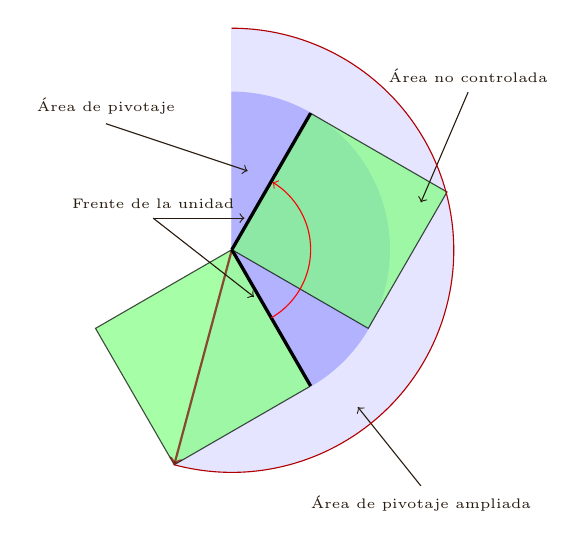
\begin{tikzpicture}[scale=2]
\filldraw[blue!10,rotate=300] (0,0) -- (1,-1) arc (-45:150:1.41cm) --
cycle;
\filldraw[opacity=.7,rotate=300,green!50,draw=black] (0,0) -- (1,0) --
(1,-1) -- (0,-1) -- cycle;
\draw[opacity=.7,red!50!black,rotate=300,thick,->] (0,0) -- (1,-1);
\filldraw[blue!30,rotate=300] (1,0) arc (0:150:1cm) -- (0,0) -- cycle;
\filldraw[very thick,rotate=300] (0,0) -- (1,0);

\filldraw[opacity=.7,rotate=60,green!50,draw=black] (0,0) -- (1,0) -- (1,-1) -- (0,-1) --
cycle;
\draw[red,->,rotate=300] (.5,0) arc (0:119:.5cm);
\filldraw[very thick, rotate=60] (0,0) -- (1,0);
\draw[brown!20!black,->] (-.8,.8) node[above] {\tiny{Área de pivotaje}}
-- (.1,.5);
\draw[brown!20!black,->] (1.2,-1.5) node[below] {\tiny{Área de pivotaje ampliada}}
-- (.8,-1);
\draw[brown!20!black,->] (1.5,1) node[above] {\tiny{Área no controlada}}
  -- (1.2,.3);
\draw[red!70!black,rotate=300] (1,-1) arc (-45:150:1.41cm);
\draw[brown!20!black,->] (-.5,.2) node[above] {\tiny{Frente de la unidad}}
  -- (.08,.2);
\draw[brown!20!black,->] (-.5,.2) -- (.14,-.3);
\end{tikzpicture}
\end{minipage}

\begin{minipage}[h]{0.5\columnwidth}
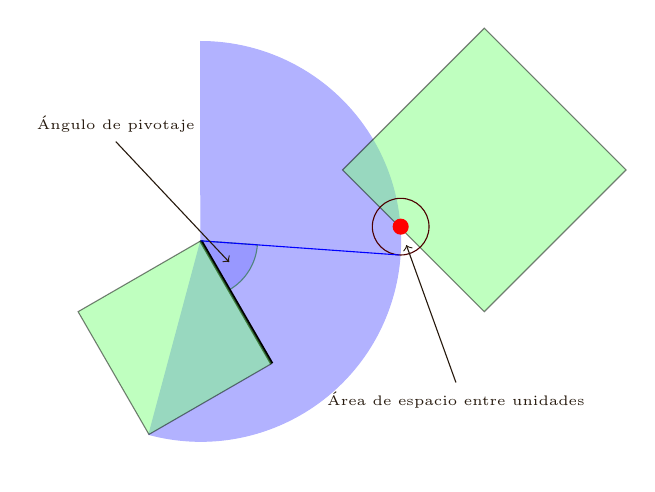
\begin{tikzpicture}[scale=1.8]
\filldraw[blue!30,rotate=300] (0,0) -- (1,-1) arc (-45:150:1.41cm) --
cycle;
\filldraw[opacity=.5,blue!50, draw=green!40!black,rotate=300] (.4,0) arc(0:56:.4cm) -- (0,0) -- cycle;
\draw[very thick, rotate=300] (0,0) -- (1,0);
\filldraw[opacity=.5,rotate=300,green!50,draw=black] (0,0) -- (1,0) --
(1,-1) -- (0,-1) -- cycle;
\filldraw[opacity=.5,green!50,draw=black] (1,.5) -- (2,1.5) --
(3,0.5) -- (2,-.5) -- cycle;
\filldraw[red] (1.41,.1) circle(1.5pt);
\draw[red!30!black] (1.41,.1) circle(.2cm);
\draw[blue] (0,0) -- (1.4,-.1);

\draw[brown!20!black,->] (1.8,-1) node[below] {\tiny{Área de espacio
    entre unidades}}-- (1.45,-.03);
\draw[brown!20!black,->] (-.6,.7) node[above] {\tiny{Ángulo de pivotaje}}-- (.2,-.15);
\end{tikzpicture}
\end{minipage}
\begin{minipage}[h]{0.5\columnwidth}
La solución adoptada es la siguiente: al igual que en el caso
anterior, para cada unidad, encontramos la intersección entre sus
aristas y la semicircunferencia de referencia de pivotaje, y también
los puntos que estén dentro de la figura. Y ahora, para cada punto,
trazamos una circunferencia de un radio de 10 unidades de
terreno. Luego tomamos los dos puntos de intersección entre dicha
circunferencia y la semicircunferencia de pivotaje: si se traza una
recta desde el origen de la semicircunferencia a dichos puntos, éstos
serán tangentes a la circunferencia \emph{de precaución}, y son éstos
puntos precisamente los que nos interesan.
\end{minipage}

De esta forma, buscamos el punto que nos de un ángulo de pivotaje
mínimo, y ese será el ángulo disponible de pivotaje actualmente.

Hay que advertir que, aunque nunca nos puede dar un ángulo
menor que 45º (puesto que la semicircunferencia de pivotaje tiene esta
cota mínima), si el valor está comprendido entre 0 y -45 (aunque
estrictamente hablando, esto no es un ángulo de pivotaje), significará
que la unidad no puede moverse porque si pivotara, entraría en
contacto con una unidad que está a su lado, pero no delante.

\subsection{Visión de una unidad}
Caracterizar la visión de una unidad, es decir, determinar qué unidad
ve a quién, es igual que caracterizar la
visión de una persona. Una persona ve un objeto cuando el espacio que
hay entre los dos está completamente libre. Si está parcialmente
ocupado también puede observarse dicho objeto, aunque la calidad de la
información que se recibe de dicho objeto es bastante menor. Si la parcialidad
de la obstaculización es muy alta, llegando a ocultar casi la
totalidad del objeto, se observará una figura de la que no
se reconocerá su forma, es decir, no se sabrá que objeto es.

Al principio, el problema de la caracterización de una unidad ignoraba
este último detalle tan importante y la vez tan simplificador. Se
intentó programar un algoritmo que admitiera una visualización directa
con tal de que el espacio no estuviera \emph{completamente}
ocupado. Es decir, que una sola recta infinitesimal de visión era
suficiente. La única forma de determinar tal tipo de visualización era
modificando el área de visión de partida.

Es decir, si partíamos de una semicircunferencia con centro en la
unidad y una amplitud de 120º de visión (siempre respecto al frente de
la unidad, porque es el frente el \emph{que ve}). Esta figura debe
entonces poderse modificar en otra figura de la complejidad que sea,
incluso dividirse en varias figuras disjuntas. Por ejemplo, un objeto
frente a la unidad de origen parte el área de visión en dos: la visión
correspondiente a los efectivos situados mas a la izquierda de la
unidad, y la visión correspondiente a los efectivos situados mas a la
derecha. Por tanto, determinar si la unidad objetivo es vista es
dividida en la determinación de la \emph{supervivencia} de dos
áreas. Si imaginamos todas las posibles situaciones nos damos cuenta
de que nos podemos encontrar ante cualquier tipo de partición y de
figura geométrica imaginable.

\begin{minipage}[h]{0.5\columnwidth}
Cuando se tuvo en cuenta el hecho de que, para observar un objeto, al
menos debe haber una franja continua de visionado, el problema se
simplificó de la siguiente forma: en vez de tener el problema de un
área modificable, y pretender que ese área nunca se haga nula (lo que
implicaría que no existe visibilidad), ahora lo resolvemos con un
descarte de áreas.

Cada área será lo que en la figura de nuestra derecha hemos llamado
\emph{haz de visión}. Un haz de visión es un rectángulo que comienza
en el frente de la unidad origen, y finaliza en una arista de la unidad de destino.
\end{minipage}
\begin{minipage}[h]{0.5\columnwidth}
\centering
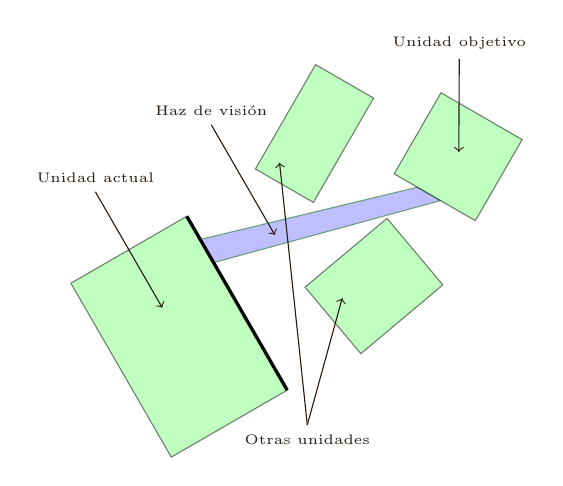
\begin{tikzpicture}[
  scale=1.7,
  rotate=300,
  unidad/.style={opacity=.5,green!50,draw=black},
  area/.style={opacity=.5,blue!50, draw=green!40!black},
  descripcion/.style={brown!20!black,->},
  ]
\coordinate (A) at (0,1);
\coordinate (B) at (1.5,1);
\coordinate (C) at (1.5,0);
\coordinate (D) at (0,0);

\coordinate (a) at (.5,2.5);
\coordinate (b) at (1.2,2.5);
\coordinate (c) at (1.2,3.2);
\coordinate (d) at (.5,3.2);

\coordinate (REF) at (a);
\coordinate (CENTRO) at (.75,1);

\filldraw[area] (0.4,1) -- (0.2,1) -- ({.5 + .2*cos(30)}, {2.5 + .2*sin(30)})--
+({.2*cos(30)}, {.2*sin(30)}) -- cycle;

\filldraw[unidad] (A) rectangle (C);

%No se por que no funciona girar coordenadas (c).
\filldraw[unidad,rotate around={30:(REF)}] (a) rectangle (1.2,3.2);

\coordinate (alfa) at (.9,1.5);
\coordinate (beta) at (1.4,2.4);

\filldraw[unidad,rotate around={10:(alfa)}] (alfa) rectangle (beta);

\filldraw[unidad,rotate around={30:(-.5,2.4)}] (0,1.5) rectangle
(-.5,2.4);

\draw[descripcion] (-.5,.5) node[above]{\tiny{Unidad actual}} --
(.5,.5);
\draw[descripcion] (-.5,1.5) node[above]{\tiny{Haz de visión}} --
(.45,1.5);

\coordinate (refunidades) at (1.8,1);

\draw[descripcion] (refunidades) node[below]{\tiny{Otras unidades}} --
(1.11,1.7);

\draw[descripcion] (refunidades) -- (0,1.8);

\draw[very thick] (A) -- (B);

\coordinate (refunidadobjetivo) at (0,3.35);

\draw[descripcion] (refunidadobjetivo) node[above]{\tiny{Unidad
    objetivo}} -- (.6,3);
\end{tikzpicture}
\end{minipage}

Tanto la base, en la unidad de origen, como su arista opuesta en la
unidad de destino, tienen un tamaño de 5 unidades de terreno, pues
esta ha sido la cota elegida para caracterizar la visión de una
unidad.

Lo que hacemos, en general, es crear todos los
posibles haces de visión entre la unidad origen y la unidad
objetivo. Esto entraña un problema. Por ejemplo, si nos fijamos en la
figura de referencia, la unidad de origen podrá ver, como mucho, dos
aristas de la unidad de destino. El nuevo problema que surge con este
planteamiento es el de caracterizar la arista o aristas
características de visión. Este problema se resuelve tal y como
muestra la siguiente figura.

\begin{minipage}[h]{0.4\columnwidth}
\centering
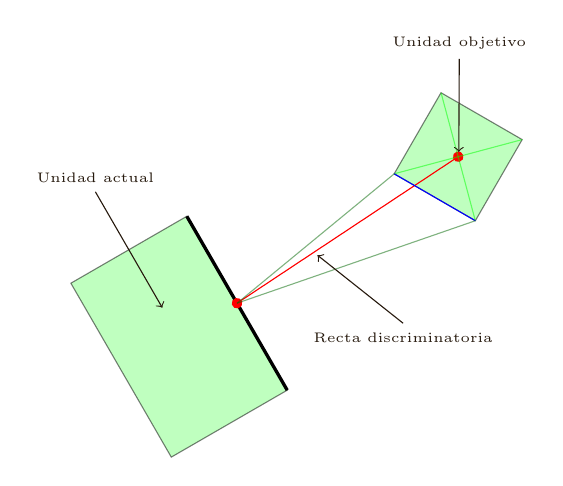
\begin{tikzpicture}[
  scale=1.7,
  rotate=300,
  unidad/.style={opacity=.5,green!50,draw=black},
  area/.style={opacity=.5,blue!50, draw=green!40!black},
  descripcion/.style={brown!20!black,->}
  ]
\coordinate (A) at (0,1);
\coordinate (B) at (1.5,1);
\coordinate (C) at (1.5,0);
\coordinate (D) at (0,0);

\coordinate (a) at (.5,2.5);
\coordinate (b) at (1.2,2.5);
\coordinate (c) at (1.2,3.2);
\coordinate (d) at (.5,3.2);

\coordinate (REF) at (a);
\coordinate (CENTRO) at (.75,1);

\filldraw[unidad] (A) rectangle (C);

%No se por que no funcioan girar coordenadas (c) no funciona.
\filldraw[unidad,rotate around={30:(REF)}] (a) rectangle (1.2,3.2);
\draw[very thick] (A)--(B);

\filldraw[red,rotate around={30:(REF)}] (CENTRO) circle(1pt) -- (intersection of a--1.2,3.2
and 1.2,2.5--.5,3.2) circle(1pt);
\draw[opacity=.5,green, rotate around={30:(REF)}] (a)--(1.2,3.2);
\draw[opacity=.5,green, rotate around={30:(REF)}] (1.2,2.5)--(.5,3.2);

\draw[blue, rotate around={30:(REF)}] (a)--(1.2,2.5);
\draw[area] (CENTRO)--(a);
\draw[area, rotate around={30:(REF)}] (CENTRO) -- (1.2,2.5);

\draw[descripcion] (-.5,.5) node[above]{\tiny{Unidad actual}} --
(.5,.5);

\coordinate (refunidadobjetivo) at (0,3.35);

\draw[descripcion] (refunidadobjetivo) node[above]{\tiny{Unidad
    objetivo}} -- (.6,3);

\draw[descripcion] (1.5,2) node[below]{\tiny{Recta discriminatoria}}
-- (.74, 1.7);
\end{tikzpicture}

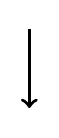
\begin{tikzpicture}
\draw[very thick, black, ->] (5,1) -- (5,0);
\end{tikzpicture}

\begin{tikzpicture}[
  scale=1.7,
  rotate=300,
  unidad/.style={opacity=.5,green!50,draw=black},
  area/.style={opacity=.5,blue!50, draw=green!40!black},
  descripcion/.style={brown!20!black,->},
  decoration = {
    markings,
    mark=at position .50 with {\arrow[red, line width = 1.5pt]{>};} }
  ]
\coordinate (A) at (0,1);
\coordinate (B) at (1.5,1);
\coordinate (C) at (1.5,0);
\coordinate (D) at (0,0);

\coordinate (a) at (.5,2.5);
\coordinate (b) at (1.2,2.5);
\coordinate (c) at (1.2,3.2);
\coordinate (d) at (.5,3.2);

\coordinate (REF) at (a);
\coordinate (CENTRO) at (.75,1);

\filldraw[area,opacity=.3,rotate around={30:(REF)}] (CENTRO) -- (.5,3.2) --
(1.2,2.5) -- cycle;
\filldraw[area,black!80,rotate around={30:(REF)}] (.5,3.2) --
(1.2,2.5) -- (1.2,3.2) -- cycle;

\filldraw[unidad] (A) rectangle (C);

%No se por que no funcioan girar coordenadas (c) no funciona.
\filldraw[unidad,rotate around={30:(REF)}] (a) rectangle (1.2,3.2);
\draw[very thick] (A)--(B);

\draw[red, rotate around={30:(REF)}] (1.2,2.5)--(.5,3.2);

\draw[blue, rotate around={30:(REF)}] (a)--(1.2,2.5);
\draw[blue, rotate around={30:(REF)}] (a)--(.5,3.2);
\draw[red, rotate around={30:(REF)},postaction={decorate}] (CENTRO) --
(1.2,2.5);

\draw[descripcion] (1.5,2) node[below]{\tiny{Área de referencia}}
-- (.74, 2);
\draw[descripcion] (0,3.5) node[above]{\tiny{Área oculta}} --
(.6,3.15);
\draw[descripcion] (-.27,1.4) node[above]{\tiny{Diagonal
    discriminatoria}} -- (.63,2.96);
\end{tikzpicture}
\end{minipage}
\begin{minipage}[h]{0.6\columnwidth}
Proyectamos, desde el centro del frente de la unidad de origen, un
segmento que acabe en el centro del rectángulo de la unidad de
destino. A esa recta la llamaremos recta discriminatoria. Esa recta
deberá intersecar con alguna arista de la unidad de
destino. A esa arista la llamaremos arista discriminatoria.

Luego, desde el centro del frente, proyectamos dos nuevos segmentos,
que acaben respectivamente en los extremos de la arista
discriminatoria. Nos quedamos, en este caso, con el segmento de mayor
longitud, situación que nos lleva a la segunda figura.

Una vez determinado el segmento mayor, elegimos la diagonal de la
unidad enemiga que coincida con su extremo con dicho segmento. A esta
diagonal la llamaremos, finalmente, diagonal discriminatoria.

Esta diagonal es importante porque divide a la unidad objetivo en dos
mitades, una que está frente a la unidad origen, y otra que
está \emph{oculta}. Las aristas que estén delante de la diagonal
discriminatoria serán las que queden descubiertas a la unidad
origen. Se puede observar como estas aristas están dentro del
\emph{área de referencia} que hemos construido proyectando el centro
del frente ha la diagonal discriminatoria.
\end{minipage}

Y ahora hacemos la última observación importante. Si intentamos
construir todos los haces de visión posibles con respecto a las
aristas descubiertas, y también, y ésta es la novedad, con respecto a la diagonal de
referencia, nos damos cuenta de que, con solo hacer que la unidad vea
a la diagonal de referencia, nos basta para admitir que ve a la unidad
original.

El método, pues, será explorar una a una todas las unidades de la
partida (de media, unas 10 o 15 unidades)
para cada rectángulo de referencia (que de media, serán entorno a unas
60), buscando intersecciones que descarten a dichos rectángulos, y, en
cuanto encontremos un haz de visión libre, abortamos la búsqueda y
admitimos que la unidad de origen vé a la unidad de destino.

\subsection{Movimiento de carga}
El movimiento de carga se resuelve de forma muy parecida al problema
de la visión, al menos en su planteamiento inicial. Evidentemente,
para cargar, la unidad tiene que ver a su objetivo. Y además, solo
podrá cargar a uno de los flancos que estén dentro de su 
visión. Y en este sentido, es donde se reenlaza este problema con el
anterior:

\begin{itemize}
\item Se obtienen las aristas \emph{descubiertas} vistas en la sección
  anterior.
\item Se buscan todas las posibles posiciones de carga en dichas
  aristas.
\item Se asegura que una posición sea accesible mediante una carga.
\item Se sigue buscando hasta encontrar una posición que también sea
  accesible, y que sea mejor, usando los criterios impuestos por el
  reglamento de \gom sobre los movimientos de carga.
\item Se desplaza la unidad a dicha posición.
\end{itemize}

Las distintas posiciones en las que es posible efectuar una carga
también es similar al caso anterior. En cada arista descubierta, voy
\emph{deslizando} un segmento del mismo tamaño que el frente de la
unidad, a intervalos de 5 en 5 unidades de terreno. Cada posición,
representa una posible posición de carga. Además, como los rangos de
ocupacion de las unidades son siempre múltiplos de 5, de esta forma se
exploran todas las posibles situaciones útiles.

Para calcular si el espacio de carga está disponible, sencillamente,
formamos un rectángulo como resultado de unir los extremos de ambos
segmentos: el frente de la unidad, y el nuevo frente virtual de la
nueva y posible posición de carga. Si dicho rectángulo está libre y si
además, la posición final también lo está, diremos que la carga es
posible. Luego tendremos que vigilar si existen mas posiciones de
carga que permitan enfrentar un número mayor de efectivos, o que se
recorra una distancia menor.

Si bien es cierto que el movimiento de carga real de la unidad no tiene
por qué coincidir con el área marcada por el rectángulo que formamos para su
representación, no nos hace falta tener en cuenta la posible área de
la unidad que pueda salirse de dicho rectángulo, por las siguientes razones:

\begin{itemize}
\item Los movimientos de carga son movimientos en partes libres y
  caóticos, y no se puede caracterizar en qué posición exacta estaría
  cada unidad en cada paso de la carga.
\item Las unidades, en la antigüedad, podían reorganizarse y
  pivotar suavemente al inicio de la carga, se podia perder levemente
  la rigidez de la formación 
  formación para hacer mas flexible su recorrido, etc. Con esto, la
  unidad tiene cierta flexibilidad a la hora de desplazar su carga,
  siendo dicho \emph{área de carga} rectángulas la mejor aproximación
  a su recorrido.
\item Y la última razón, y a su vez la mas importante, ninguna
  posición intermedia en este \emph{área de carga} será
  una posición final de la unidad, salvo la última, y la última sí que
  se comprueba.
\end{itemize}

\subsection{Movimiento de huida}
El movimiento de huida se puede ver como una variante del problema del
desplazamiento con la diferencia o particularidad de que el
desplazamiento, en vez de tener una cota máxima de movimiento, su cota
es mínima.

Es decir, en el caso del desplazamiento, se debía calcular cual era el
desplazamiento máximo que se podía realizar sin entrar en contacto con
ninguna otra unidad. En el caso del movimiento de la huida, el valor
de partida es el valor mínimo que hay que realizar, y si no hay
espacio, este valor se supera en busca de la primera posición de la
unidad que tenga el suficiente espacio libre como para que la unidad
que huye pueda \emph{estacionar}.

En general, el verdadero problema es caracterizar la posición final de
la unidad cuando existen unidades que entorpecen la huida.

Para ello, supongamos que existen unidades en el camino de huida que no
nos permiten detener a la unidad en el lugar que le corresponde según
la cantidad de movimiento de huida asignado.

Como se observa en la figura inferior, si intentasemos colocar a la
unidad en su posición adjudicada, que en la figura hemos llamado
límite de huida, la unidad se colocaría justo encima de la primera
unidad foránea existente en el camino. Tal y como indica el
reglamento, la unidad debe continuar su movimiento hasta encontrar la
primera posición libre.

\begin{minipage}[h]{.5\columnwidth}
Para ello, en cada unidad presente en el camino, trazamos un par de
rectas discriminantes para cada unidad, una justo delante suya, que
llamaremos proximal, y otra justo detrás suya, que llamaremos recta
distal. Son las que hemos puesto de color rojo en la
figura.

Para cada unidad, obtenemos el espacio que existe entre la recta
distal de la primera unidad y la recta proximal de la siguiente,
restandole 20 unidades de terreno a dicha distancia (10u por la
primera unidad, y 10u por la segunda, para respetar la distancia entre
unidades tal y como exige el reglamento de \gomf).
Si esta distancia
es mayor a la profundidad de la unidad, significará que la 
unidad cabe en dicho espacio, y la primera posición encontrada que
cumpla con estas propiedades será la posición elegida final para
colocar a la unidad que está huyendo.
\end{minipage}
\begin{minipage}[h]{.5\columnwidth}
\centering
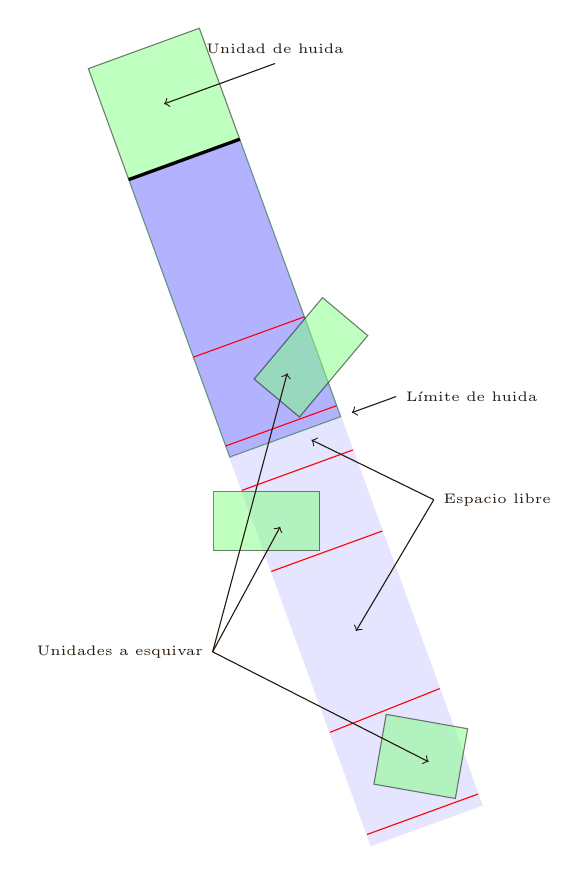
\begin{tikzpicture}[
  scale=1.5,
  rotate=200,
  unidad/.style={opacity=.5,green!50,draw=black},
  area/.style={opacity=.5,blue!50, draw=green!40!black},
  fondo/.style={blue!10},
  descripcion/.style={brown!20!black,->}
  ]

\filldraw[fondo] (0,1) rectangle (1,7);
\filldraw[area] (0,1) rectangle (1,3.5);
\filldraw[unidad] (0,0) rectangle (1,1);
\draw[very thick] (0,1) -- (1,1);
\filldraw[unidad, rotate around={30:(-.2,2.5)}] (-.2,2.5) rectangle
(.7,3);
\filldraw[unidad, rotate around={160:(1.4,4.2)}] (1.4,4.2) rectangle
(2.3,4.7);
\filldraw[unidad, rotate around={150:(.5,6)}] (.5,6) rectangle
(1.2,5.4);

\draw[red] (0,2.6) -- (1,2.6);
\draw[red] (0,3.4) -- (1,3.4);
\draw[red] (0,3.8) -- (1,3.8);
\draw[red] (0,4.53) -- (1,4.53);
\draw[red] (0,5.95) -- (1,5.98);
\draw[red] (0,6.9) -- (1,6.9);

\draw[descripcion] (-.5,.5) node[above]{\tiny{Unidad de huida}} --
(.5,.5);
\draw[descripcion] (-.5,4.43) node[right]{\tiny{Espacio libre}}
-- (.3,3.6);
\draw[descripcion] (-.5,4.43) -- (.5,5.25);
\draw[descripcion] (1.7,5) node[left]{\tiny{Unidades a esquivar}} --
(.3, 6.5);
\draw[descripcion] (1.7,5) -- (.8,4.2);
\draw[descripcion] (1.7,5) -- (.3,3);
\draw[descripcion] (-.5,3.5) node[right]{\tiny{Límite de huida}}--
(-.1,3.5);
\end{tikzpicture}
\end{minipage}
\cleardoublepage

% Este archivo es parte de la memoria del proyecto fin de carrera
% de Aarón Bueno Villares. Protegida bajo la licencia GFDL.
%
% Para más información, la licencia completa viene incluida en el
% fichero fdl-1.3.tex

% Copyright (C) 2010 Aarón Bueno Villares

\section{Pruebas}
\label{sec:pruebas}

Para diseñar los casos de prueba, distinguimos entre aquellas clases y
estructuras que, por su naturaleza, pueden ser testeadas
individualmente, de aquellas que se testean de forma integrada. La
mayoría de las funciones ofrecidas por el gestor de escenario fueron
testeadas de forma individual, al igual que todas las
estructuras matemáticas. En cambio, el resto de clases y funciones,
por su simplicidad y por su dependencia gráfica, no merecía la pena
realizar casos de prueba individuales, quizás mas complejos que
estudiar, simplemente, su comportamiento integrado. Así que, en
definitiva, la organización de los casos de prueba fue la siguiente:

\begin{enumerate}
\item A medida que se fueron implementando, se probaron
  individualmente todas las estructuras y funciones matemáticas
  diseñadas y las funciones de corte mas matemático.
\item Una vez superados los test anteriores, y a medida que se
  agregaba nueva funcionalidad, se probaba cada vez el sistema
  completo de forma integrada.
\item Al finalizar todo el proceso completo de diseño e implementación
  comenzaron las pruebas beta. Algunos usuarios probaron el producto y
  no se detectó ningún defecto adicional.
\end{enumerate}

\subsection{Pruebas alfa}
Las pruebas alfa son las pruebas que se realizan durante el proceso de
desarrollo. En el caso que nos ocupa, las pruebas se realizaban al
final de cada iteración de implementación.

\subsubsection{Pruebas unitarias}
Las funciones sustentas a este tipo de pruebas, como hemos dicho
antes, eran las mas relacionadas con el ámbito mas matemático del
juego. Debido a su complejidad, las pruebas se realizaron bajo un
enfoque estructural, es decir, de caja blanca, y además, bajo un
criterio de cobertura de sentencias, es decir, se estableció que la
mejor forma de estudiar el comportamiento correcto de una función era
lograr que al menos cada posible rama de la función fuese explorada,
con la finalidad de que al menos cada sentencia fuera ejecutada una
vez. A su vez, se diseñaron las pruebas de modo que las sentencias mas
problemáticas de cada función (aquellas que poseen divisiones,
peligros de desbordamiento, bucles o ecuaciones complejas) se probaran
varias veces explorando tanto los casos mas comunes como los mas
extremos (análisis de valores límite), de modo que se examine de forma
exhaustiva su comportamiento.

Como era de esperar, el mayor núcleo de errores de esta clase se
encontraban en la implementación de las estructuras matemáticas del
juego, que tenían alta implicación en el comportamiento del gestor de
escenarios.

\subsubsection{Pruebas de integración}
Las pruebas de integración del sistema complejo al completo (en cada
iteracción de diseño), debida a la relativa sencillez estructural de
las clases que la conformaban (una funcionalidad compleja pero formada
por un rico dinamismo de funciones individuales muy sencillas), se
realizaron bajo un enfoque funcional o de caja negra. Se probaba,
sencillamente, que la ejecución de la nueva funcionalidad
implementada, en consonancia con funcionalidades completadas previas,
realizara con éxito lo que se supone que debía realizar.

El principal núcleo de defectos encontrados bajo estas pruebas de
integración recayeron sobre el gestor de iconos, sobre el gestor de
ejércitos, y en los procesos de destrucción (cuando finaliza una
partida). 

\subsection{Pruebas beta}
Al finalizar el proceso de diseño, implementación y pruebas alfa se
ofreció el juego a distintos usuarios (generalmente compañeros de
universidad) para que probaran el juego y me remitieran los errores
producidos y el contexto del mismo. Luego repetía las situaciones
reportadas, hasta obtener el error nuevamente y explorar su origen,
corregir y reenviar la nueva versión a mis
\emph{ayudantes}. Generalmente, los fallos y defectos encontrados en
esta fase de pruebas fueron relacionadas con el proceso de huida de
las unidades desmoralizadas en combate.

\cleardoublepage

% Este archivo es parte de la memoria del proyecto fin de carrera
% de Aarón Bueno Villares. Protegida bajo la licencia GFDL.
%
% Para más información, la licencia completa viene incluida en el
% fichero fdl-1.3.tex

% Copyright (C) 2010 Aarón Bueno Villares

\section{Herramientas}
\label{sec:herramientas}

Para la realización de este proyecto se ha hecho uso de una serie de
herramientas y aplicaciones adicionales que facilitaron su desarrollo.

\subsection{GCC}
El proyecto ha sido desarrollado en el lenguaje de programación C++. Y
todo lenguaje necesita de un compilador que permita traducir el código
a código máquina, único lenguaje que la máquina comprende. Nuestro
particular traductor (mas concretamente, compilador) ha sido
GCC\footnote{\emph{GNU Compiler Collection.}}.

\emph{GCC} es un compilador de \emph{GNU}, por lo tanto libre y
abierto, que da soporte a varios lenguajes de programación, entre
ellos \emph{C++}. Pertenece al llamado \emph{GNU toolchain}, el
conjunto de herramientas de \emph{GNU} por y para la programación.
 
\subsection{libSDL}
Todo juego tiene una gran cantidad de elementos de interacción con el
usuario. Para ello, se debe tener acceso al hardware, de modo que
obtengamos información de todos los eventos de usuario producidos.

La librería SDL\footnote{\emph{Simple DirectMedia Layer.}} ha sido la
piedra angular del aspecto multimedia de nuestro juego. Lo hemos usado
principalmente para nuestra interacción con el sistema de video, y los eventos de teclado y
ratón. A su vez, hemos usado las siguientes librerias auxiliares de
\emph{SDL}:
\begin{description}
\item[SDL\_image:] Usado para la carga de imágenes (permite trabajar con
  imágenes de cualquier formato, mientras que \emph{SDL} solo permite
  cargar imagenes \emph{bmp}).
\item[SDL\_mixer:] Usado para nuestro trato con audio.
\item[SDL\_gfx:] Usado para rotar y redimensionar nuestras imágenes.
\item[SDL\_ttf:] Usado para imprimir texto en pantalla.
\end{description}

\subsection{GIMP}
\emph{GIMP}\footnote{\emph{GNU Image Manipulation Program.}} es otra
herramienta del proyecto \emph{GNU}. Como su nombre indica, es un
editor y manipulador de imágenes. Con él hemos creado (y/o modificado
a partir de otras imágenes libres) todos los iconos, los menus, las
peanas de las unidades, y en general, toda imagen y todo elemento
gráfico del juego a pasado por manos de \emph{GIMP}, bien para su
retoque, bien para su creación.

\subsection{GNU Emacs}
Richard Stallman junto a Guy Steele creó, en 1975,
el editor de textos Emacs\footnote{Editor MACroS}. Mas tarde, entre
1984 y 1985, se lanzó \emph{GNU Emacs}, una nueva versión derivada de
la anterior diseñada por Richard Stallman para el proyecto
\emph{GNU}. Hoy en día es considerada por muchos programadores como el
mejor editor de textos, y existen una gran diversidad de modos de
emacs que proveen diversos entornos de desarrollo para prácticamente
casi todos los lenguajes de programación.

Nuestro proyecto ha sido prácticamente desarrollado al completo en él.

\subsection{SVN}
Este proyecto dispone de un repositorio donde siempre hemos mantenido
actualizado el desarrollo del proyecto. \emph{SVN}\footnote{\emph{SubVersioN}.} ha sido la
herramienta auxiliar utilizada para interactuar con el repositorio,
actualizar las versiones, y mantener nuestra copia de seguridad del proyecto.

Las herramientas como \emph{SVN} proveen un mecanismo de control de
versiones cuando existen varios desarrolladores involucrados, evitando
que se destruyan cambios y ordenando las distintas modificaciones que
se van realizando en el proyecto, permitiendo tener acceso a
anteriores versiones de cada fichero involucrado en el proyecto, así
como del proyecto en su conjunto. Como este proyecto ha
sido desarrollado únicamente por mí, no se ha aprovechado
completamente la potencia de esta herramienta, pero aun así me ha
permitido tener acceso directo a mi proyecto desde cualquier máquina,
y tener acceso, además, a todas la versiones enviadas, que en varias
ocasiones me ha permitido recuperar versiones antiguas de ciertos
ficheros que he necesitado recuperar.

\subsection{Make}
\emph{Make} es una herramienta que hemos usado para la automatización
de la compilación del proyecto. \emph{Make} permite crear scripts,
comúnmente en un fichero llamado \emph{makefile}, para declarar las
dependencias de los distintos módulos, a fin de acelerar la
compilación (dependencias sin modificaciones no se recompilan) y
aumentar la robustez de la misma.

En nuestro proyecto, además de compilar el proyecto, a través de
\emph{make} podemos generar la documentación y la memoria del proyecto
(véase abajo), así como limpiar de forma directa todos los ficheros
intermedios e innecesarios creados en el proceso de compilación tanto
del proyecto como de la memoria.

\subsection{LaTeX}
\emph{TeX} fue concebido inicialmente por Donald Knuth a principios de la década de los
80 para construir un lenguaje de programación de edición
profesional de textos científicos, y ya en 1984 Leslie Lamport
desarrolló \emph{LaTeX} como un conjunto de macros que orientaban \emph{TeX}
a la edición de cartas, libros, y en general, a la edición de textos
desde un mayor nivel de abstracción.

Este proyecto ha hecho uso de este lenguaje para la construcción completa
de la memoria.

\subsection{Doxygen}
\emph{Doxygen} es una herramienta ideada para documentar código de
varios lenguajes de programación. Provee una serie de comandos, dentro
de los llamados \emph{comentarios de Doxygen}, que Doxygen sabe
interpretar y que luego usa para generar un documento html, pdf o rtf
(según los deseos del usuario) con la documentación del código,
haciendo uso además de \emph{Graphviz} y \emph{TeX} para generar gráficos de
dependencias entre clases y módulos, y proveer la inclusión de
fórmulas matemáticas en la documentación resultante.

Nuestro proyecto ha hecho uso de ésta herramienta para documentar el
código.

\subsection{Umbrello}
\emph{Umbrello} es una herramienta de apoyo para el desarrollo
software, sobre todo bajo un paradigma orientado a objetos, que
permite hacer un análisis y un diseño bajo el estándar UML, obtener
los diagramas UML mediante ingeniería inversa a partir de código
nativo, o automatizar parte de la implementación del software
creando el código a partir de los diagramas UML diseñados.

Se ha usado esta herramienta para realizar los diagramas UML de la
memoria.
% Este archivo es parte de la memoria del proyecto fin de carrera
% de Aarón Bueno Villares. Protegida bajo la licencia GFDL.
%
% Para más información, la licencia completa viene incluida en el
% fichero fdl-1.3.tex

% Copyright (C) 2010 Aarón Bueno Villares

\chapter{Conclusiones}
\label{chap:conclusiones}

\gom ha sido mi primer proyecto. Y es evidente que su realización no
me iba a dejar indiferente. No ha sido nada fácil construir una idea
clara sobre lo que me dispondría a hacer, no ha sido nada fácil
poner en práctica dicha idea, así como tampoco ha sido nada fácil
solucionar los problemas del camino. Por último, no ha sido nada fácil
realizar esta memoria.

En total, he aprendido varias cosas:
\begin{enumerate}
\item No hay que dejarse seducir por las mas sabrosas ideas, y mucho
  menos intentar sostenerlas sin premeditación. Quizás hubiera sido
  mas suave la realización de este proyecto si desde el primer momento
  hubiese pretendido crear un software simple e ir haciendolo mas
  complejo de forma progresiva, en vez de empezar por una idea inicial
  compleja que luego tuve que simplificar.

\item He aprendido lo importante que es un buen reparto del trabajo, y
  lo importante que es probar cada parte de forma independiente, en
  vez de intentar conseguir que un sistema integrado funcione de forma
  conjunta.

\item Es crucial ver la diferencia y la naturaleza de un proyecto con
  volumen, frente a un proyecto de pequeña escala como a los que
  hemos estado acostumbrados en el transcurso de los años
  académicos. Sobre la utilidad de la ingeniería del software en este
  aspecto, se podrían decir muchas cosas. Lo que sí es seguro es que
  una metodología tiene un fundamento sólido basado en la experiencia,
  y como dicen nuestras abuelos y abuelas, la experiencia es un
  grado. En un proyecto de corto volumen, se puede abarcar la
  totalidad del problema con sencillez. Papeles en sucio, garabatos y
  esbozos son los máximos representantes de esta clase de
  situaciones. Y \gom no se puede realizar con papeles en sucio,
  garbatos y esbozos. Hace falta el prisma del orden. Y quizás esa sea
  la lección más importante aprendida con la realización de este
  proyecto: las metodologías son orden en la realización de
  proyectos software, y ese orden es necesario cuando el problema
  abarca una conjunto amplio de ideas.
\end{enumerate}

Espero que este proyecto sea respaldado en un futuro, aunque sea
lejano, por un grupo respetable de seguidores aférrimos. Y aun sin
conseguir este propósito, el valor de lo aprendido en esta realización
compensa la posible y no descartable soledad de mi criatura. Entre
tanto, intentaré potenciar mi producto para hacerlo mas extenso,
incrementar su calidad, su riqueza en funcionalidad, así como su
belleza artística. Solo espero no ser el único, y que con el paso del tiempo mas
desarrolladores se animen en mi travesía de construir este videojuego,
que, según alcanza mi documentación, hasta hoy es único en su género.

\section{Mejoras futuras}
\label{sec:mejoras}

A continuación, presento una lista de mis ideas a largo plazo de mejoras por y para el proyecto.

\subsection{\ldots de interfaz}
Me interesa mucho el diseño 3D. Uno de los posibles objetivos de
mejora del producto es pasar la interfaz a tridimensional, y añadirle
animaciones.

Y del mismo modo que en \textit{WF}, los jugadores se compran, modelan
y pintan sus miniaturas, también sería posible y muy atractivo crear
un modo de pintura, de modo que, al diseñar un usuario un ejército,
pueda elegir obtenerlo como una matriz de efectivos y unidades sin
vida ni color, y que el usuario decida qué aspecto darle. Es decir,
potenciar al máximo la personalización de su propio ejército. 

\subsection{\ldots de dominio}
En este tramo es donde me surgen un conjunto mas rico de
ideas. Resultaría muy interesante que \gom fuera inteligente, en el
sentido de que \gomf, mas que un juego, pueda ser un propio jugador al
que poder enfrentarse. Quizás con una red neuronal, algoritmos
evolutivos o diseñando un sistema selectivo se pueda conseguir
implementar dicho juego inteligente, de modo que dicho
\textit{jugador virtual} sea entrenado en cada batalla contra la
máquina por el propio jugador real, y así la máquina, con el paso del
tiempo, se convierta en el alterego del usuario. Incluso se podrían
exportar los perfiles conseguidos y enfrentarlos a otros
\textit{alterego's} de otros usuarios. Sería, además, una bonita y
objetiva forma de ver quien de los dos usuarios es mejor maestro en el
arte de la guerra.

También sería deseable añadir un buen soporte de red, para poder crear
concursos e incluso campañas (con mapas de conquista inclusive) de
forma que distintos jugadores reales intenten competir de diversas
formas con otros jugadores reales, cada uno desde su propio
hogar. Esto último provocaría la atractiva idea de crear una página
web, o un foro, donde se pudiesen hacer quedadas, comentar
estrategias, así como mostrar y comentar partidas previas entre otros
jugadores.

Y, por supuesto, el reto innamovible e incuestionable es la de
enriquecer constantemente la funcionalidad del reglamento, el número
de ejércitos, la diversidad de las unidades, o el tipo y formato de
las reglas.

\subsection{\ldots de datos}
No hay nada mas enriquecedor que el autoexámen. Entonces también, y
por último, tengo en mente crear una buena base de datos que guarde la
información de cada partida completada con éxito, y así generar
estadísticas, detectar buenas y malas jugadas en un turno concreto, o
algún movimiento mal escogido, para que así un jugador pueda evaluar
sus propias participaciones y descubrir sus propios progresos y
avances como maestre táctico.

No sería difícil, en este punto, permitir que el usuario pueda
exportar, en forma de imágenes o documentos, representaciones
esquemáticas de partidas concretas (con gráficos sencillos que
representen cada unidad y cada movimiento, ataques, cargas, etc).

\section{Contacto}
\label{sec:contacto}
Para contactar conmigo, envíe un correo a
\emph{abv150ci@gmail.com}. Tambien puede visitar la página web oficial
del proyecto en \emph{https://forja.rediris.es/projects/gom/}, desde
donde podrá obtener mas información, las fuentes e imágenes usadas en
la realización de \gomf, así como poder estar al tanto de las
novedades producidas en su desarrollo.


%%%%%%%%%%%%%%%%%%%%%%%%%%%%%%%%%%%%
%%     Desenlace
%%%%%%%%%%%%%%%%%%%%%%%%%%%%%%%%%%%%
\backmatter

% Este archivo es parte de la memoria del proyecto fin de carrera
% de Aarón Bueno Villares. Protegida bajo la licencia GFDL.
%
% Para más información, la licencia completa viene incluida en el
% fichero fdl-1.3.tex

% Copyright (C) 2010 Aarón Bueno Villares

\chapter{Reglamento}
\phantomsection
\label{reglamento}

\begin{center}
{\bf\large Preámbulo}

\begin{minipage}{12cm}
{\small
Este documento describe el reglamento general aplicado en cada uno de
los pasos de la resolución de una partida en \gom, versión 1.0. Así,
aquí se incluyen las reglas aplicadas sobre movimiento, combate, disparos
o magia. Este documento debe tenerse presente siempre y de forma estricta a la hora de organizar un ejército o una táctica, pues ideas que requieran actos no regidos en este reglamento no se podrán hacer efectivos en la partida.}
\end{minipage}
\end{center}

\section*{Introducción}
\label{introduccion}
\gom pretende ser una simulación de escenarios en los que poder llevar
a cabo tácticas militares, con un corte medieval y fantástico. Este reglamento es completo, y contiene
todas las reglas aplicables del juego. Nada de lo expresado fuera de
este documento, será legal en una partida de \gomf, y si en algún lugar relacionado con el proyecto oficial de \gom se afirma algo que contradiga cualquier cosa aquí escrita, siempre tendrá mas validez la versión de este reglamento.

\subsection*{Panorámica general}
\gom permite enfrentar a dos ejércitos en una batalla campal. Al igual
que en las batallas históricas, un ejército está formado por unidades,
y el objetivo es organizar dichas unidades para conseguir la
victoria. Y es por ello que \gom es un juego de táctica militar. El
corte u ambiente del juego es medieval y fantástico, y las unidades y
los ejércitos tienen un comportamiento en el campo de batalla que los
asemeja a las batallas que se protagonizaban en el medievo (que son
herencia del paradigma de guerra de la antiguedad clásica) o como vemos en las guerras de muchas películas de
fantasía, y que son muy distintas a como se llevan a cabo las guerras
en la actualidad.

Es por ello que se desea rescatar este espíritu tomando forma en un
juego orientado a su reproducción en un medio digital, paradigma que,
en el mundo de los videojuegos, no consta de ningún ejemplar. El
reglamento en sí sirve para que cualquier jugador pueda generar
batallas militares incluso en su propio salón, con papeles, o con
miniaturas diseñadas. \gom es independendiente de la finalidad
práctica que se le de a este reglamento.

\subsection*{Mecánica del juego}
El juego está organizado en turnos, y consta de dos ejércitos formados
por unidades. Un jugador efectúa su turno de
juego y luego el oponente juega el suyo, hasta 6 turnos por jugador. A
su vez, cada turno de cada jugador está organizado en tres fases a
resolver en orden: movimiento, combate y disparos.

\paragraph{Confección y despliegue}
Una vez ambos jugadores hayan confeccionado sus propios ejércitos y
hayan decidido una posición inicial para cada una de sus unidades,
desplegarán sus tropas en su zona de despliegue (dependiendo de quién
se haya asignado el rol de jugador 1 y quién de jugador 2) y podrá comenzar la batalla.

\paragraph{Unidades, atributos y características}
Cada unidad tiene una serie de atributos que definen las
particularidades de la naturaleza interna de cada uno de los efectivos
de una unidad. Existen
diversos atributos, como movimiento o fuerza. A su vez una unidad
puede tener una serie de características, que no dependen de la
naturaleza de la unidad, sino generalmente de su equipaje o
complementos de la unidad (o también del tamaño de los efectivos),
estas características son la salvación por armadura, la fuerza de
arma, el alcance de arma, la potencia y el rango de ocupación.

\paragraph{Turnos de juego}
Se realizarán hasta seis turnos alternos por jugador. Cada turno contiene tres fases, que se detallarán a continuación:

\begin{enumerate}
\item \textit{Movimiento}
Como su nombre indica, aquí es dónde se permite \emph{elegir} qué movimientos y cargas pueden efectuar tus unidades. Es la fase con mas reglas y restricciones.

\item \textit{Combate}
Si dos o mas unidades se encuentran en un combate, se resolverán en
esta fase, para cada jugador.

\item \textit{Disparos}
Aquellas unidades que dispongan de armas de proyectiles, podrán
disparar a otras unidades enemigas.

\end{enumerate}

\paragraph{Fin de la partida}
Una vez que finalicen los cinco turnos, la partida se anunciará como
finalizada. Se calcula quien ha sido mejor comandante y la categoría de su victoria.

\subsection*{Vocabulario}
\label{vocabulario}
\subsubsection*{Escala}
Aunque los jugadores podrán (y deberían) aplicar cualquier escala
deseada -siempre en proporción a la aquí indicada-, este reglamento
contabilizara todas sus medidas espaciales en unidades que llamaremos
unidades de terreno o simplemente \textit{u}. \textit{u} podrá ser
tanto un metro, como un pixel, como una pulgada (o si apetece, un
kilómetro). Esto ya recae sobre la decisión de los propios
usuarios. Con respecto a los costes económicos de las unidades, a cada
unidad de coste, o también puntuación, se le designara sencillamente con el calificativo \textit{p}. Así, por ejemplo, una unidad de caballeria ocupa un frente de 10u, un lado de 20u, y un coste de 35p.

\subsubsection*{Ejércitos}
\gom enfrenta a dos ejércitos. Un ejército está formado por unidades,
y una unidad por efectivos. El efectivo será el elemento básico de
cada ejército.

\subsubsection*{Despliegue}
Desplegar es el hecho de elegir una posición inicial para cada una de
las unidades de un ejército. Se le denomina fase o tiempo de
despliegue al hecho de colocar las unidades en el campo de batalla,
según el despliegue elegido.

\subsubsection*{Combatientes}
Existirán dos jugadores por partida, y cada uno comandará uno de los
ejércitos enfrentados. Después de que cada jugador haya elegido su
ejército y confeccionado su despliegue, decidirán quién responderá
como jugador 1, y quién como jugador 2. En este sentido, el ejército
es independiente de la partida, y un jugador podrá confeccionar un
ejército y su correspondiente despliegue de forma aislada, y luego
usarlo para diversas partidas diferentes. Lo que no podrá decidir de
forma aislada será su orden de jugador (jugador 1 o jugador 2) que
dependerá de cada partida y del acuerdo llegado con el oponente. 

\subsubsection*{Escenario}
\gom deberá jugarse sobre una superficie de 1.280u de ancho por 600u
de alto, que será llamado escenario o campo de batalla. El formato del
escenario sera apaisado, es decir, que el eje x del escenario mide los
1.280u de ancho, y el eje y mide los 600u de alto. El eje x se expande
de izquierda a derecha, y el eje y en dirección sur-norte.

El escenario se divide en tres secciones rectángulares paralelas al
eje x. La primera se expande en las primeras 100u del eje formando
un rectángulo de 1.280u por 100u. Se denominará zona de despligue
uno, y será la zona de despliegue correspondiente al primer jugador o
ejército. La segunda se expande desde 100u hasta las 500u en el eje y. Será
la que divida a ambos ejércitos al inicio del combate. La tercera se
expande desde las 500u hasta completar el escenario, en las 600u. Se
denominará zona de despligue dos y será la zona de despliegue
correspondiente al segundo jugador.

\subsubsection*{Turnos y fases}
Una partida se organiza en turnos. Se realizarán 6 turnos completos
para cada jugador, de forma alterna. Es decir, el orden será el
siguiente: \textit{Turno 1 del jugador 1}, \textit{Turno 1 del jugador
  2}, \textit{Turno 2 del jugador 1}, \ldots, \textit{Turno 5 del
  jugador 2}.

Cada turno de cada jugador se divide en tres fases, fase de
movimiento, fase de combate y fase de disparos, y deberán jugarse en ese orden. 

\subsection*{Razas}
Cada ejército será de una raza, y existen dos razas distintas: orcos y
humanos. Cada raza define un conjunto de unidades distinto con un
perfil de atributos propio. El conjunto concreto de unidades definidas
en cada raza vendrá expresado en un apartado especial al final de éste
reglamento.


\section*{Atributos y características}
\label{atributos}
Una batalla está compuesta por una gran diversidad de unidades de distinta naturaleza. En \GoM la naturaleza de cada unidad se modula mediante unos valores llamados atributos y unas características. 

\subsection*{Atributos}
\paragraph{Movimiento (M)}
Es el desplazamiento básico de una unidad en un turno de juego. Si una unidad posee un atributo de movimiento M10, significará que su desplazamiento básico es de 10u.

\paragraph{Habilidad de armas (HA)}
La habilidad que tiene cada efectivo de una misma unidad en combate
cuerpo a cuerpo. Está ponderada de 0 a 10. 

\paragraph{Habilidad de proyectiles (HP)}
La habilidad que tiene cada efectivo en el disparo con armas de proyectiles. Está ponderada de 0 a 10. 

\paragraph{Fuerza (F)}
Este atributo mide la fuerza de cada efectivo de una misma unidad en combate cuerpo a cuerpo. Ponderada de 0 a 10.

\paragraph{Resistencia (R)}
Es la dureza del cada efectivo de una misma unidad en combate cuerpo a cuerpo. Ponderada de 0 a 10.

\paragraph{Ataques (A)}
El valor de este atributo indica cuántos ataques tiene un guerrero en
un solo turno de combate.

\paragraph{Heridas (H)}
Este atributo pondera la dificultad para matar a un efectivo de la
unidad. Es un valor mayor que 0. Si un efectivo recibe un número de
impactos igual a su valor de heridas, se considerará una baja y el
efectivo deberá retirarse del juego.

\paragraph{Iniciativa (I)}
Indica el reflejo y rapidez de cada efectivo de una misma unidad en combate cuerpo a cuerpo. Ponderada de 0 a 10.

\paragraph{Liderazgo (L)}
El liderazgo indica la valentia de una unidad. Ponderado de 0 a 10.

\subsection*{Características}
Por otro lado, existen otros valores llamados
\emph{características}. Estos son la potencia, la salvación por
armadura, la fuerza de arma, alcance del arma y el rango de ocupación.En general estos
atributos no son propios de la naturaleza o el entrenamiento del
guerrero, sino más bien de factores externos como armaduras o el peso
que infiera la unidad en la batalla, como por ejemplo, la fuerza
adicional que da ir montado en un caballo. También se incluye como
característica el coste de una unidad.

\paragraph{Potencia (P)}
La potencia es el peso o valor (en sentido figurado) que tiene cada
efectivo de una misma unidad en batalla. Por ejemplo un efectivo
montado a caballo tiene más potencia que un efectivo de infantería, y
a su vez un orco en jabalí tiene más potencia que un humano a pie. La
potencia de una unidad es la potencia sumada de cada uno de sus
efectivos.

\paragraph{Salvación por Armadura (SA)}
La salvación por armadura de una unidad es la dificultad que imponen
sus armaduras, escudos o cascos a la hora de recibir, cada efectivo de
una misma unidad, un golpe. Ponderado de 0 a 10.

\paragraph{Fuerza de arma (FA)}
Es la fuerza que poseen las armas de proyectiles de una
unidad. Funciona igual que el atributo fuerza, pero solo actúa en la
resolución de disparos. Está ponderado de 0 a 10.

\paragraph{Alcance de arma (AA)}
Es el alcance que poseen las armas de proyectiles de una unidad. Sus
valores toman la misma forma que el atributo movimiento.

\paragraph{Rango de ocupación (RO)}
Cada efectivo tiene un \emph{rango de ocupación}, este rango de
ocupación es el espacio que ocupa la presencia del efectivo en el
campo de batalla (el suelo que pisa), que refleja el espacio ocupado
por el efectivo en el mapa. El rango de ocupación de cada efectivo
tiene siempre forma rectángular, y tanto su ancho como su alto es
múltiplo de 5u.

Por ejemplo, un efectivo de una legión de un ejército humano tiene un rango de ocupación de 10ux10u, y un efectivo de caballería un rango de ocupación de 10ux20u (el primer valor indica el rango de ocupación en el eje x del efectivo, y el segundo el rango de ocupación en su eje y).

\paragraph{Coste en puntos}
Existirá una última característica crucial llamada puntuación de un efectivo. Cada efectivo de una misma unidad tiene un mismo coste en puntos. El coste en puntos de una unidad será la suma del coste en puntos de cada uno de sus efectivos. El coste en puntos de cada efectivo de cada unidad está diseñado de modo que sea coherente y equilibrado con el resto de sus atributos y características, por ejemplo, una mejor HA y un alto liderazgo dará al efectivo un coste en puntos mayor que un efectivo con un valor menor en estos atributos.

\subsection*{Perfil de atributos}
Cada unidad del juego vendrá definido por un perfil de valores para cada una de los atributos y características definidas en el apartado anterior, en forma de tabla.

\subsection*{Chequeo de atributos y características}
\label{chequeo}
La mayoría de los atributos pueden ser puestos a prueba durante la partida. Hay dos tipos de chequeos, los que son puesto en común con el adversario, o los chequeos individuales de los atributos.

\subsubsection*{Chequeo individual}
Los atributos y características sustentas a chequeo individual son todas aquellas que se han indicado como ponderadas de 0 a 10. Esto representa un porcentaje. Cuándo se hace un chequeo individual, se genera un número aleatorio entre 0 a 10, si el número generado es mayor que el valor actual del atributo o característica, se falla el chequeo, en caso contrario se supera. Sin embargo, si el número obtenido es 0, se falla el chequeo sin importar el valor del atributo, y si el valor obtenido es 10, se supera el chequeo automáticamente. Esto significa que una miniatura de I0 solo superará su chequeo de iniciativa cuando el número aleatorio obtenido sea 10. Estas reglas evitan que una unidad con un atributo o característica con el valor máximo o  mínimo siempre falle o supere respectivamente su chequeo individual.

\subsubsection*{Chequeo comparativo}
Los atributos y características sustentas a chequeo comparativo son todas aquellas que se han indicado como ponderadas de 0 a 10. Un chequeo comparativo es el hecho de chequear el valor de un atributo o característica de un efectivo con respecto al valor de un atributo o característica de otro efectivo. Cuando comparas dos atributos o características, siempre hay un atributo o característica agente y un atributo o característica pasiva. Por ejemplo, si un orco ataca a un humano y se debe comparar su F con la R del humano, el atributo agente será F, y el atributo pasivo será R. Lo que se hace en estos casos es restarle al atributo agente, la diferencia entre el atributo agente y pasivo. Por ejemplo, si el ataque fue de F4, y la resistencia del objetivo es R5, la diferencia entre ambos valores es 1, entonces el valor modificado del atributo agente F, será 4-1 = 3. Una vez modificado el valor, se hace un chequeo individual del valor modificado.

\section*{Unidades}
\subsection*{Formación de una unidad}
\label{formacion}
Hemos dicho que una unidad está formada por efectivos. Estos efectivos no se pueden organizar de cualquier forma, tienen que hacerlo de manera que formen una unidad bien formada. La formación de una unidad se llama formación en bloque.

Una formación en bloque puede tener, en principio, cualquier número de
efectivos, que deberán situarse unos junto a otros (los rangos de
ocupación de los distintos efectivos son contiguos). La formación debe
tener siempre forma de cuadro, es decir, posee filas con un mismo
número de efectivos y alineados, como una matriz, salvo la última fila
que puede tener cualquier número de componentes si por número no se
consigue llenar entera. Si se consigue llenar, cualquier nuevo
efectivo añadido a la unidad deberá colocarse en la fila
inmediatamente posterior exáctamente detrás y alineado con un efectivo
de la fila anterior. Los efectivos de la última fila deben estar
siempre lo mas centrados posible. Por ejemplo, una unidad con un ancho
de 5 efectivos, y una última fila de 3, tendrá a sus efectivos de la
última fila colocados en las posiciones 2-3-4 (está centrado puesto
que queda un \textit{efectivo libre} a cada lado).

Por último, si el número de efectivos de la última fila no es adecuado
para conseguir que esté centrado (por ejemplo, que el ancho de la
unidad sea de 5 efectivos, y solo haya 2 en la última fila), se
colocarán mas a la izquierda que a la derecha.  Por ejemplo una unidad
con 21 efectivos y un ancho de fila de 6, tendrá 3 filas de 6
efectivos alineados, y una última fila de 3 efectivos colocados en las
posiciones 2-3-4, en vez de 3-4-5. 

Las unidades también tienen un número mínimo de efectivos y un número
máximo. Estos valores son restricciones de confección de
ejército. Al elegir una unidad en el diseño de su ejército, el número
de efectivos elegidos estará comprendido entre dicho número mínimo y
dicho número máximo \refreg{confeccionejercito}. Evidentemente, en el
transcurso de la partida, el número
mínimo de efectivos se reducirá siempre que sea necesario. Cuando
llege a cero, la unidad habrá sido aniquilada. El número máximo de
efectivos no puede superarse puesto que no existen reglas que aumenten
el número de efectivos en el transcurso de la partida.

El número mínimo de efectivos que debe tener cualquier unidad en la
primera fila (y por simple aplicación de la regla anterior, también el
mínimo de efectivos que debe tener cualquier fila de la unidad; salvo
la última), son 4 efectivos, a no ser que el número mínimo de
efectivos (el mencionado en el párrafo anterior) sea también menos que
cuatro. Si la unidad tiene menos de 4 efectivos, por ejemplo 3,
obviamente no hay nada que hacer y la unidad se queda con un ancho de
fila de 3 unidades. Si se añaden nuevos efectivos a la unidad, se
deben de rellenar, como mínimo antes de crear una nueva fila, tantos
efectivos como queden para completar una fila de 4.

El encaramiento de la unidad será unívoca. Esto es, que todos los
efectivos de una unidad de bloque mirarán en una misma dirección. Esto
se reduce a decir que el encaramiento de la unidad vendrá dada por el
encaramiento de su primera fila. La primera fila es la que siempre
dirige a la unidad completa, y cualquier efectivo en filas secundarias
o posteriores no tienen ningún derecho de mando en ninguno de los
sentidos. Esto significa que a la hora de que la unidad efectúe
cualquier acción, será la primera fila la que mande, y será la
visibilidad de la primera fila la que importe \refreg{visibilidad}.

La primera fila de una unidad se llamará frente, la última
retaguardia, la primera columna flanco izquierdo, y la última columna
flanco derecho. Los efectivos se cuentan de izquierda a derecha. Es
decir, que el primer efectivo será el efectivo situado mas a la
izquierda de la primera fila, y el último efectivo de la unidad será
el situado mas a la derecha de la última fila.

\subsection*{Visibilidad de una unidad}
\label{visibilidad}
La visibilidad de un efectivo dentro de una unidad viene dado por su encaramiento. Su
ángulo de visión será de hasta 60º grados a su izquierda y de hasta
60º hacia su derecha, es decir, un ángulo de visión total de 120º. La
línea de visión izquierda se proyecta desde la esquina superior
izquierda del rango de ocupación del efectivo con un ángulo de
inclinación de 60º respecto a la perpendicular de su
frente. Análogamente, la línea de visión derecha se proyecta desde la
esquina superior derecha del rango de ocupación del efectivo con un
ángulo de inclinación de -60º respecto a la perpendicular de su
frente. La visión total del efectivo será el área encerrada por ambas
líneas de visión. Los efectivos situados en filas posteriores de la
unidad se considera que no ven nada, y la visibilidad de la unidad
será la suma de la visibilidad de cada efectivo de su frente, es
decir, será el área encerrada entre la línea de visión izquierda del
primer efectivo del frente y la línea de visión derecha del último
efectivo del frente de la unidad.

En este punto, el primer requisito para que una unidad vea a otra es
que dicha unidad esté dentro, al menos parcialmente, del área de
visión.

El segundo factor que delimita la visibilidad de un efectivo o unidad
son los obstáculos de un terreno o la presencia de otras
unidades. En este punto, para que una unidad vea a otra, basta con
encontrar un segmento del frente de la unidad, de 5u de tamaño, otro
segmento en una arista de la unidad de destino, también de un tamaño
de 5u, y conectar los extremos formando un cuadrilatero. Si existe al
menos un cuadrilatero de estas características que esté completamente
libre, es decir, que ni siquiera esté parcialmente ocupada por ninguna
otra unidad, la unidad estará viendo a dicha unidad objetivo.

En realidad, cuando un cuadrilatero de estas características está
parcialmente ocupado, no significa que la unidad no pueda ver que hay
``mas allá'', solamente que la unidad no es capaz de identificar qué
está viendo, y en este sentido, el ``ver'' y el ``caracterizar'' se
confunden con este criterio, pues las situaciones en la que es
necesario saber si una unidad ve a otra también es necesario admitir
que la unidad sabe efectivamente que lo que está viendo es una unidad enemiga, ya que
va a realizar una carga o un disparo.

El hecho de elegir ese ``ancho'' de 5u de visión es una medida
arbitraria suficiente para caracterizar la visión de una
unidad. Ampliar o disminuir este ancho, sería equivalente a exigir
un mayor o menor grado de calidad de la visión para caracterizar
cuando una unidad \emph{reconoce} a otra.

\section*{Preámbulos a una batalla}
Antes de comenzar una partida, hace falta elegir una raza, diseñar un
ejército, su despliegue y colocar las tropas en el campo de batalla en
su lugar asignado correspondiente.

\subsection*{Confección de un ejército}
\label{confeccionejercito}
Para confeccionar un ejército se elige una raza, y por último, se
elige un conjunto de unidades con un número determinado de efectivos
en cada una (que podrá variar de una unidad a otra) y la cantidad de
efectivos inicial en el frente de la unidad, según los definidos por
la raza elegida y las restricciones que ésta imponga. El tamaño en
puntos del ejército es libre, en el sentido de que se podrá
confeccionar un ejército tan grande como se desee. Las únicas
restricciones al tamaño del ejército son las impuestas por las
dimensiones del escenario, y en concreto, por la zona de despliegue,
es decir, todo el ejército debe caber en la zona de despligue. Tampoco
se recomienda diseñar un ejército con demasiadas unidades, pues
podría limitar la maniobrabilidad. El tamaño impuesto para un
escenario de \gom es lo suficientemente amplio como para manejar desde
ejércitos pequeños a ejércitos mucho mas modestos.

Además, la confección de un ejército va íntimimamente ligada a la
confección de su despliegue, y estas dos propiedades de un ejército
deben idearse juntas. La confección de un ejército no se da por
concluida hasta que el despliegue del mismo no esté diseñado.

Por último, una unidad tendrá siempre unas restricciones respecto al
número mínimo y número máximo de efectivos con los que la unidad podrá
desplegarse. En la descripción en las listas de ejército se indicará
cuales son estos valores para cada unidad. En la confección del
ejército, no se podrán diseñar unidades con un número de efectivos de
despliegue distinto a este intervalo de valores impuesto.

\subsection*{Confección del despliegue}
\label{despliegue}
Desplegar es posicionar al ejército en el campo de batalla antes de
que ésta comience. Se impone que toda unidad despliegue mirando hacia
el frente, se decir, con un ángulo de 0º respecto al eje x. Esto
provoca la deseable situación de que los dos ejércitos comiencen
frente a frente. A su vez, se impone, evidentemente, que toda unidad
despliegue en su zona de despliegue \refreg{vocabulario}. Como la confección del ejército
es independiente de una partida concreta (los ejércitos serán
\textit{reusables}), no se puede suponer nada acerca de la zona de
despliegue asignada. Es por tanto inadmisible intentar confeccionar un
ejército conforme a una información que se conocerá luego. Por tanto,
confeccionar el despliegue equivale a confeccionar un despliegue con
la suposición añadida de que el jugador será el primero. Si luego
resulta no serlo, solo hace falta desplegar las tropas en su posición
simétrica respecto al campo de batalla.

Por lo tanto, el único dato que se debe especificar al diseñar el
despliegue de cada unidad únicamente será la posición de la unidad en
el campo de batalla, y esto se hará declarándo la coordenada respecto
al eje x e y de la esquina superior izquierda de la unidad; como la
unidad se despliega recta, y el rango de ocupación, número de
efectivos y frente de la unidad es conocido, la posición final de la
unidad es inequívoca. Evidentemente, en el despliegue, toda unidad
debe estar comprendida dentro de su zona de despliegue, al
completo. Esto implica que no podrá colocarse ninguna unidad total ni
parcialmente fuera de dicho espacio. Por ejemplo, una unidad de frente
ancho cuya esquina superior derecha se declare muy cerca del borde
derecho, podrá dejar la parte derecha de la unidad fuera de la zona de
despliegue, y en general, fuera del campo de batalla. Esta es una
situación que ha de controlarse. Unidades con demasiadas filas también
pueden escapar parcialmente de la zona de despliegue.

\subsection*{Organización de una partida}
\label{organizacionpartida}
Una batalla es única y exclusivamente el enfrentamiento de dos
ejércitos. Esto implica un previo acuerdo entre los dos jugadores que
harán de comandantes para ambos ejércitos. Los dos ejércitos,
evidentemente, podrán ser tanto de la misma raza como de razas
distintas. Por otro lado, los dos ejércitos no tienen ninguna
restricción respecto a su valor en puntos, es decir, que podrán
enfrentarse, si así lo desean los jugadores, y sobre todo, si así de
valiente es el primer jugador, ejércitos de 1.000p contra
3.000p. Luego, los jugadores deben ponerse de acuerdo para establecer
quien será el jugador 1, y quién el jugador 2. Despues del despliegue,
el jugador 1 será el que comienze la partida y luego el jugador 2 le seguirá.

\subsection*{Configuración del escenario}
\label{escenario}
La elementos de escenografía a elegir, y su posición en el escenario
es delimitada con las siguientes dos restricciones. La primera es que
los elementos de escenografía no podrán situarse en la zona de
despliegue, y la segunda es que dichos elementos no podrán tampoco
estar a menos de 40u de dichas zonas de despliegue.

Además, el terreno ocupado por los elementos de escenografía se considerará
terreno impasable (es decir, que las unidades no podrás atravesar
dicha zona). Respecto a si dificultará o no la visión de otras unidades,
debería depender de la naturaleza del elemento de escenografía, pero se deja libertad a este efecto. 

Una vez elegido la cantidad y el tipo de los elementos de
escenografía, se colocarán antes del despliegue a través del escenario de forma aleatoria o
decidida, pero siempre respetando las dos restricciones anteriomente impuestas.

\subsection*{Turno de despliegue}
\label{despliegue}
Una vez acordados los ejércitos, comprobada su similitud en puntos, y
su correcta planificación de despliegue, cada jugador coloca sus
unidades correctamente en su zona de despliegue correspondiente, de
modo que toda unidad de cada ejército esté encarada con la línea de
batalla del ejército enemigo, y cuya esquina superior izquierda
coincida con la planificada en el diseño del despliegue.

El jugador segundo se encuentra ante una pequeña dificultad. Tal y
como se comentó en el apartado de confección del despliege, ambos
jugadores debieron suponer que serían el jugador primero. Como
consecuencia, la colocación de sus unidades según sus coordenadas le
llevará a colocarlas en la zona de despliegue del primer jugador. Para
soslayar esta dificultad, solamente hay que desplegar al ejército
segundo en la segunda zona de despliegue a partir de las coordenadas
diseñadas para la zona de despliegue primera, bajo la siguiente
regla: \[(x,y)=(1280 - x, 600 - y)\]

De este modo, se obtendrá la situación simétrica del ejército del
segundo jugador respecto a la zona de despliegue uno. Otra solución
sería considerar momentáneamente a la esquina superior derecha del
escenario como nuevo origen de coordenadas, y desplegar las tropas tal
cual vienen especificadas en la propia lista de ejército. El efecto es
equivalente.

Al proceso de despliegue, y al tiempo transcurrido desde ese momento,
hasta el comienzo del primer turno por el primer jugador, se le
denominará turno de despliegue o turno 0.

\section*{Turnos y fases de juego}
\label{turnos}
Una vez desplegados los ejércitos, puede comenzar la batalla. El
esquema de partida es muy simple, el jugador primero comienza el turno
primero, y realiza su fase de movimiento, y acto seguido, su fase de
combate, para finalizar con su fase de disparo. Una vez terminado, el
jugador segundo comienza su primer turno, y procede de la misma
forma. Luego el jugador primero realiza su segundo turno, y así
sucesivamente hasta que ambos jugadores hayan completado
satisfactoriamente 6 turnos completos de juego. Acto seguido se
calcula la categoría y dirección de la victoria, y finaliza la
partida.

Mas esquemáticamente, un turno de un jugador se divide en el siguiente
juego de fases y subfases:
\begin{itemize}
\item Inicio de turno
\item Fase de movimiento
\begin{itemize}
\item Declaración de cargas
\item Movimiento de cargas
\item Resto de movimientos
\end{itemize}
\item Fase de combate
\begin{itemize}
\item Resolución de combates
\item Efecto de los combates
\end{itemize}
\item Fase de disparo
\end{itemize}

Se describirá cada fase mas concisamente en las secciones que vienen a
continuación.

\subsection*{Inicio de turno}
\label{inicioturno}
El inicio de turno no corresponde una fase por sí misma. Solamente es
un espacio inicial de turno reservado para realizar ciertas acciones
sobre las unidades que huyen \refreg{huidas}.

En el inicio de turno se tiene que comprobar, para cada unidad del
ejército cuyo turno esté en curso, si puede reagruparse. En caso de no
conseguirlo, deberá continuar con su movimiento de huida \refreg{reagrupamiento}. El orden en
que se resuelvan estas huidas no importa, y se realizan en cualquier
orden deseado.

\subsection*{Fase de movimiento}
\label{fasemovimiento}
En esta fase es en donde las unidades que no estén huyendo del
ejército cuyo turno esté en curso podrán moverse libremente. Está
compuesta por las siguientes subfases:

\begin{itemize}
\item Declaración de cargas
\item Movimiento de cargas
\item Resto de movimientos
\end{itemize}

\subsubsection*{Declaración de cargas}
En esta subfase es donde las unidades pueden declarar sus cargas \refreg{dinamica}. Se
declaran en un orden preciso que hay que anotar, ya que de este orden
dependerá muchas de las acciones posteriores \refreg{declaracion}.

\subsubsection*{Movimiento de cargas}
En esta subfase se mueven todas las cargas en el mismo orden en que
fueron delcaradas. Para mover una carga, hay primero que verificar si
la unidad llegará a su objetivo. Luego, si efectivamente se verifica
que la carga será posible, se efectúa la carga \refreg{cargar}. Si no, se efectúa un
movimiento de carga fállida \refreg{cargafallida}.

\subsubsection*{Resto de movimientos}
En esta subfase es donde el usuario puede mover sus unidades, y en
cualquier orden, de forma libre. Aquí las unidades podrán marchar
\refreg{marcha} y realizar maniobras \refreg{maniobras}.

\subsection*{Fase de combate}
\label{fasecombate}
Esta fase está diseñada para resolver los combates existentes en la
partida desde turnos anteriores, o generados en la fase de movimiento
gracias a nuevas cargas \refreg{combate}. Se divide en las siguientes dos subfases:

\begin{itemize}
\item Resolución de combates
\item Efecto de los combates
\end{itemize}

\subsubsection*{Resolución de combates}
La fase de resolución de combates es la fase donde se resuelven todos
los combates existentes en la partida actual.

Los combates deberán resolverse en el mismo orden relativo en el que
fueron creados, según su antigüedad \refreg{ordencombates}. Cada
combate se ejecuta según la iniciativa de cada una de las unidades involucradas, y de la
antigüedad de sus participantes \refreg{resolucion}.

Para cada combate, se anota su resultado según un criterio de
puntuación, que luego se establecerán, nuevamente, en el mismo orden
que los mismos combates fueron resueltos, en la subfase de efecto de
los combates \refreg{resultadocombate}.

\subsubsection*{Efecto de los combates}
En esta subfase se generan los efectos de los combates. Se pueden
identificar tres tipos de efectos: desmoralización, efectos mágicos y
disolución de combates \refreg{resultadocombate}.

La desmoralización es referida a las unidades que han perdido el
combate, con su posible correspondiente huida \refreg{huidas}. Los efectos mágicos,
referidas a los ganadores \refreg{magia}. La disolución de un combate es el hecho de
que ese combate finalice. Si no lo hace, el combate queda vigente
hasta la fase de combate del turno del siguiente jugador.

\subsection*{Fase de disparo}
\label{fasedisparo}
En esta fase las unidades que posean armas de proyectiles podrán
disparar a unidades enemigas \refreg{disparo}. El orden de los disparos es libre, y
para cada unidad que decida disparar, los disparos y sus consecuencias
se ejecutan inmediatamente a continuación. Luego, si se desea, una
nueva unidad podrá disparar, y se efectuarán sus consecuencias antes
de comenzar con una tercera unidad, y así tantas veces como se desee.

\section*{Reglas de movimiento}
\label{movimiento}
En esta sección se presentan todas las reglas referidas al
movimiento. El movimiento no solo está presente en la fase de
movimiento, ya que, por ejemplo, el reagrupamiento pertenece a la
dinámica del movimiento de las unidades en \gomf, sin embargo
este movimiento se efectua en la fase de inicio de turno, y no en la
fase de movimiento. Es por ello que en esta sección se explican las
reglas \emph{generales} de movimiento, aplicables en distintas
situaciones de una batalla.

\subsection*{Movimiento}
Moverse es el hecho de que una unidad cambie de posición en el
escenario (por ejemplo, que pivote) o de estado de movimiento (por
ejemplo, que su movimiento sea de marcha). Los desplazamientos o
cambios de posición siempre tienen un coste, y éste se mide en
unidades de terreno. El movimiento de una unidad viene dado, principalmente, por la
capacidad M del guerrero. A mayor valor de atributo M mas se podrá
mover la unidad en el terreno de juego en un solo turno. 

El efecto de los desplazamientos o cambios de posición en una unidad
es el siguiente. Si una unidad tiene una capacidad de desplazamiento
Mx, y la unidad realiza un desplazamiento de coste u, a la unidad le
quedarán x-u unidades de terreno para el siguiente turno. En la
práctica, se considera que la capacidad dee desplazamiento de una
unidad es un valor continuo en vez de discreto. Así, una unidad podrá
desplazarse, si lo desea, 5.12u para que le resten 4.88u durante el
resto del turno.

Los movimientos de huida no están sujetas a estas restricciones, y
tienen sus propias reglas de desplazamiento \refreg{huidas}. Éstas huidas deben
desplazarse con independencia de lo que le reste de movimiento a la
unidad en un turno.

En general, la unidad se mueve en dirección frontal, es decir, que en
el transcurso de movimiento no se debe variar el ángulo que hay entre
la cara frontal del rango de ocupación y la linea de dirección en que
se esté moviendo, que siempre deberá ser de 90º.

¿Esto significa que las unidades solo pueden mover hacia delante?,
sería descabellada tal absurdez. Para que una unidad pueda cambiar su
encaramiento, o su ángulo de giro, hay ciertas maniobras que lo
permiten. Así, por ejemplo, para que una unidad se quiera mover en una
dirección de 45º con respecto a su posición frontal, deberá antes
hacer un pivotaje de 45º y luego desplazarse frontalmente. Estos
pivotajes y resto de maniobras pueden hacerse tanto como se deseen en
el transcurso del movimiento \refreg{maniobras}.

Y por último, una unidad que se mueva fuera del campo de batalla jamás
volverá y representa el abandono total de la partida, por lo cual la
unidad deberá considerarse baja a todos los efectos.

\subsection*{Terreno}
El terreno es el tipo de suelo que hay en cada parte del escenario. Hay dos tipos de terrenos: terreno abierto, y terreno impasable.

\subsubsection*{Terreno abierto}
Es el terreno común y normal del juego, y las unidades tendrán un movimiento libre regido por las normas habituales de movimiento del juego (las regidas en esta sección del manual).

\subsubsection*{Terreno impasable}
En un terreno impasable, las unidades, directamente, no podrán pasar y
se consideran obstáculos a todos los efectos. Estos terrenos deben ser
bordeados y nunca se podrán atravesar. Los únicos terrenos impasables
corresponden, en concreto, a todos los elementos de escenografía
situados en el escenario.

\subsection*{Espacio entre unidades}
\label{espacio}
Es importante recalcar que a toda unidad debe respetarse el rango de
ocupación de cada uno de esos efectivos. Así, durante el movimiento, y
en general bajo cualquier situación, menos en un combate, toda unidad
debe esquivar a las restantes, porque eso se reduciría a colisionar o traspasar rangos de
ocupación durante el movimiento.

Hace falta mencionar una regla importante que siempre, y para esto no
hay excepción posible, debe respetarse entre unidades de distintos
bandos. Para que dos unidades se consideren trabadas en combate hemos
dicho que antes hay que declararles carga y luego cargar. Por eso
ninguna unidad puede acercarse demasiado a una unidad enemiga, ya que
si llegan a tocarse, deben luchar (es ilógico e irreal que dos
enemigos estén uno frente al otro y no combatan), y esto solo es
posible hacerse si se declara una carga. Así que es norma que dos
unidades enemigas entre sí siempre deban de estar separadas como
mínimo, a no ser que sea para combatir, una distancia de 10u. Para
unificar el criterio, y como dos unidades, por cuestiones de
maniobrabilidad, tampoco pueden estar juntas, se impondrá que dos
unidades amigas también respeten esta distancia.

\subsection*{Maniobras}
\label{maniobras}
Las maniobras son los movimientos de desplazamiento voluntario
característicos de la subfase de resto de movimiento. Existen tres
tipos de maniobras: desplazamiento, pivotaje y giro.

Para poder realizar una maniobra, la unidad debe estar completamente
libre, es decir, no debe estar huyendo ni trabada en combate.

\subsubsection*{Desplazamiento}
\label{desplazamiento}
Desplazamiento es el hecho de que una unidad cambie su posición a base
de mover hacia delante, sin cambiar su ángulo con respecto al eje x
del escenario. Es decir, siguiendo una dirección perpendicular hacia
delante.

El coste de este movimiento es, precisamente, la distancia que hay
entre los frentes de la posición actual de la unidad, y la nueva. Una
unidad nunca podrá desplazarse una distancia mayor que la restante por
su capacidad de movimiento, es decir, según su atributo de movimiento
menos la distancia ya recorrida o gastada por otras maniobras en el
mismo turno.

\subsubsection*{Pivotaje}
\label{pivotaje}
Pivotar una unidad es cambiar su encaramiento. Para pivotar una unidad
hay dos posibilidades, bien pivotarla a la derecha (para mirar al
este), bien pivotarla a la izquierda (para mirar al oeste), todo
depende del eje escogido. Si se coge como eje el pivote superior
izquierdo de la unidad, el pivotaje será izquierdo (se mantiene fijo
ese eje y se mueve la unidad como un compás). Y recíprocamente para el
pivotaje derecho con eje derecho.

Un pivotaje izquierdo consume un movimiento igual al recorrido por el
último efectivo de la linea frontal de la unidad, es decir, el situado
en la esquina superior derecha. Un pivotaje derecho consume un
movimiento igual al recorrido por primer efectivo de la linea frontal
de la unidad, es decir, el situado en la esquina superior
izquierda. En ambos casos, dicho recorrido es igual a la longitud del
arco realizado por el efectivo indicado en cada caso. Esto quiere
decir que si una unidad con M20 y un frente de 5 efectivos mueve 10u,
y se realiza un pivotaje derecho donde el efectivo quinto se desplaza
5u, a la unidad completa le quedarán otros 5u para completar, si lo
desea, su movimiento, bien desplazándose frontalmente, bien con otra
maniobra como un nuevo pivotaje. Cabe destacar que contra mas ancha
sea la unidad (mas efectivos existan en el frente), mas costoso será
su giro para un mismo ángulo, pues se recorrerá un arco mayor.

\subsubsection*{Giro}
\label{giro}
Un giro no desplaza realmente a la unidad, aunque sí que consume
movimiento. Un giro es simplemente cambiar el frente de la unidad a su
retaguarda. Si la unidad miraba al frente (no puede mirar a otro sitio), la unidad
ahora puede girar para que su retaguardia sea su nuevo
frente. Los efectivos no se mueven, solamente se giran.

Al girar la unidad, su última fila será su nuevo frente. Si la última
fila no estaba completa, se completa usando efectivos de la primera
fila, de modo que, al girar la unidad, la nueva última fila (la que
antes era el frente) tenga a sus efectivos en la misma
posición relativa que los efectivos de la última fila antes del
giro. Lo importante es mantener a la formación de la unidad sin modificaciones.

Una unidad solo podrá girar si no está marchando, y una vez girada, no
podrá marchar en lo que queda de turno.

\subsection*{Movimiento de marcha}
\label{marcha}
El movimiento de marcha representa un movimiento a la carrera, que
incrementa temporalmente el atributo M (solamente para ese turno de
movimiento). El movimiento de marcha de una unidad es el doble de su
capacidad de movimiento actual. Además, como ya se ha dicho, una unidad que
haya girado no podrá marchar en su fase de movimiento, o una unidad
que esté marchado no podrá girar en lo que quede del mismo.

A su vez, si la unidad ha marchado, en la fase de disparo tendrá
penalizaciones en sus disparos de la fase de disparo, si es que llega
a realizar alguno.

\subsection*{Dinámica de cargas}
\label{dinamica}
Las cargas son el único mecanismo posible para que varias unidades
puedan entablar combate \refreg{combate}. Poseen dos subfases correspondientes para
declararlas y ejecutarlas en la fase de movimiento, y por cada carga
realizada con éxito se enriquecerá posteriormente la fase de combate.

\subsubsection*{Declaración de cargas}
\label{declaracion}
La declaración de la carga es tan fácil como indicarle a un oponente
que deseas cargar. Solo se puede declarar una carga a una unidad
visible \refreg{visibilidad}. Estas declaraciones se hacen en su subfase de
movimiento correspondiente \refreg{fasemovimiento}.

Antes de declarar carga no se permite medir el terreno de juego y en
\gom no hay ningún medio para hacerlo. Se debe ponderar a ojo si se cree
que la unidad llegará a cargar o si por el contrario fallará la
carga. Una unidad que desea cargar puede declarar carga a una sola
unidad, aunque una unidad enemiga puede ser objetivo de varias
unidades, que se establecerán en declaraciones independientes.

Es importante ser cuidadoso ponderando el éxito de carga de tu unidad,
pues un error de cálculo puede hacer que la carga sea fállida
\refreg{cargafallida} y colocar a tu unidad en una situación poco
ventajosa.

Por último, solo pueden declarar carga aquellas unidades que no estén
combatiendo ni huyendo, y si una unidad declara carga, no podrá
realizar ninguna acción mas durante el resto de su turno, salvo disparar.

\subsubsection*{Movimiento de la carga}
\label{cargar}
En la subfase de movimiento de cargas se intenta establecer, por cada
declaración realizada y respetando el mismo orden, si cada unidad,
gracias a su movimiento, llega a su objetivo. La cantidad de movimiento
disponible para cada unidad que carga es del doble de su atributo
actual M. Dos o mas unidades que declaren una carga contra
una misma unidad, deberán resolver sus movimientos en el mismo orden,
con la posibilidad de que el movimiento de la primera carga (que
intentará maximizar su posición, véase mas abajo), podrá impedir el
éxito de la segunda. Se recomienda que solo se declaren varias cargas
a una misma unidad cuando haya espacio suficiente para todos.

Por ejemplo, que haya tantos \emph{flancos} libres (en sentido general, es
decir, incluyendo frente y retaguardia) como cargas quieran
declararse; es por ello que mas de cuatro cargas contra una misma
unidad es desaconsejable, a no ser que la unidad enemiga sea muy
grande y haya el suficiente espacio.

Por otro lado, es importante resaltar que no se puede elegir el flanco
al que se desea cargar, solamente se declara la unidad a la que
atacar. Para establecer si la unidad llega al objetivo y de qué forma
se sigue el método presentado a continuación.

Solo puede cargarse a los flancos que estén \emph{delante} de la línea
característica de visión \refreg{visibilidad}. De entre esos
flancos, siempre hay que calcular en qué posición se traba mas
efectivos, siempre y cuando se llege a esa posición. Dicho de otro
modo, de entre todas las posiciones a la que la unidad puede cargar,
se elige la que maximice el número de efectivos que se trabarán en
combate \refreg{efectivoscombatientes}. Evidentemente, en ese caso debe
violarse la condición de la separación entre unidades, pues dos
unidades solo están trabadas cuando están en contacto.

A la posición final (el segmento) donde la unidad de carga se ha alineado con la
unidad enemiga la llamaremos posición de carga. Es inmediato que el
tamaño de este segmento es el del frente de la unidad. Para saber si una
unidad \emph{llega} a una posición de carga, se traza una recta desde
el centro del frente de la unidad al centro de la posición de
carga. Si el tamaño de este segmento es menor que el movimiento
disponible de carga, la unidad llega a dicha posición, de lo
contrario, si esa posición de carga es la única posible, la carga será
fállida \refreg{cargafallida}. Si no es la única posible, hay que buscar otra.

Tampoco será válida una posición de carga si el espacio que existe
entre el frente de la unidad y la posición de carga está ocupado,
aunque sea parcialmente. Esto se reduce a considerar un cuadrilatero
formado tras unir los extremos de los segmentos frente y posición de carga, y verificar que dicho espacio
esté completamente libre.

De entre todas las posibles
posiciones de carga, hay que buscar la que trabe en combate el máximo
número de efectivos. Esto se hace sumando el número de efectivos
trabados para cada unidad, y no solo para la unidad que ha
cargado. Por ejemplo, si la unidad objetivo tiene efectivos con un
RO muy ancho en su eje x, pero poco profundo en su eje y, será mas
óptima la carga por su flanco puesto que la suma en bruto de efectivos trabados
será mayor.

\subsubsection*{Carga fállida}
\label{cargafallida}
Si la carga ha sido fállida, el movimiento a realizar se considera un
movimiento obligatorio. Este movimiento se ejecuta en el mismo momento
en que se sepa que no existe ninguna posición de carga efectiva, es
decir, justo antes de validar el movimiento de la siguiente carga,
respetando el orden de las declaraciones.

Cuando una carga es fállida, se debe realizar un movimiento como
máximo igual al tercio del movimiento de carga, de forma rectilinea (es decir, un
movimiento hacia adelante). Si el espacio que la unidad tiene delante
está ocupado, se desplazará hasta la posición máxima sin violar la
separación entre unidades \refreg{espacio}.

\subsection*{Huidas}
\label{huidas}
Huir es el hecho de que una unidad se vea envuelta en el pánico y
decida abandonar el combate. Los movimientos de huida se realizan en
ciertas ocasiones en las que la situación se ha vuelto peligrosa para
la misma. En esta sección se regulan las reglas acerca de qué
situaciones son las que ocasionan ``peligro'' para la unidad, y como
se han de desplazar esas huidas.

\subsubsection*{Unidades que huyen}
\label{unidadhuye}
Las situaciones en las que una unidad está sustenta a huir son las siguientes:

\begin{enumerate}
\item Cuando una unidad comenzó a huir en turnos anteriores y todavía
  no se ha reagrupado \refreg{inicioturno}.
\item Cuado la unidad es desmoralizada en combate. Su movimiento de
  huida se realiza en la subfase de efectos del combate, dentro de la
  fase de combate \refreg{fasecombate}.
\item Cuando la unidad pierde mas de un 25\% de sus efectivos en la
  fase de disparo enemiga \refreg{fasedisparo}.
\end{enumerate}

Las unidades que estén en las dos primeras situaciones, deberán
realizar un chequeo de liderazgo antes de ver si efectivamente se
declaran como unidades que huyen. Si se falla este chequeo, la unidad
realizará su movimiento de huida \refreg{huidas}. A partir
de entonces (tercer caso), en el siguiente \emph{inicio del turno} de su jugador, tendrá que realizar
otro movimiento de huida, a no ser que se reagrupen \refreg{reagrupamiento}.

En el caso de que deban huir por desmoralización en combate, para
realizar el chequeo de liderazgo, existen unos modificadores al
liderazgo antes de realizar el chequeo \refreg{resultadocombate}.

Cuando una unidad huye, hay cierta probabilidad de que sus atributos
sean modificados (negativamente), por efecto de la magia \refreg{magia}.

\subsubsection*{Movimiento de huida}
\label{movimiento de huida}
El movimiento de huida depende básicamente de la capacidad de
movimiento básico de la unidad que huye. Esta cantidad de movimiento
de huida es aleatorio en cada turno de huida. Si la capacidad de
movimiento de una unidad es M, su movimiento de huida en el turno
actual es la media de la suma de tres resultados aleatorios
comprendidos entre la mitad de n y su triple. Por ejemplo, si la
capacidad de movimiento de una unidad es de 10, y está huyendo, tres
resultados aleatorios posibles entre 5 (mitad) y 30 (triple) son 7,
16, 22, y la media de esas tres cantidades es 15, así que ese turno
moverá 15. Esto pondera el hecho de que en un movimiento de huida,
este es desorganizado, sin formación y sustento a tropiezos, caídas,
cansancio (que pueden disminuir la velocidad de la huida), o pánico
excesivo (que pueden aumentarla), además fomenta el hecho de que la
huida no es controlable por el jugador.

En un movimiento de huida, la unidad que huye intentará por todos los
medios escapar de la situación que le produce peligro. La dirección
del movimiento de huida siempre es en el sentido opuesto a la unidad
que le produce peligro. Si debe huir por motivo de los disparos,
huirá en dirección contraria a dicha unidad. Si es por motivos de un
combate, huirá de la unidad de mayor potencia de entre todas las
unidades enemigas que participen en el mismo combate. Si la huida no
ha sido recién lanzada (es decir, que es del tercer tipo de entre los
anunciados en el apartado anterior), el movimiento de huida continuará
la misma dirección que en los turnos anteriores. En la siguiente
sección se explica el método usado para elegir la dirección y el
comienzo del movimiento de huida.

Si en el movimiento de huida se encuentra a otra unidad, pasará por
encima suya sin modificar su dirección. Si el valor obtenido en su movimiento de huida no
es lo suficientemente alto como para saltar completamente a la unidad,
se otorga la bonificación necesaria para traspasarlo. Si justo detrás
de esa unidad existen otras unidades, se otorga la bonificación
necesaria al movimiento hasta encontrar la primera posición, en la
misma dirección de huida, donde la unidad quepa completamente sin
violar las restricciones de cercanía a otras unidades (10u). Si el
elemento es de escenografía, se aplican los mismos criterios.

Si la unidad por la que ha pasado es amiga, ésta unidad realizará un
chequeo de liderazgo. Si lo falla, deberá huir en dirección contraria
a la unidad que le provoca el pánico, es decir, en dirección contraria
a dicha unidad. Si es enemiga, la unidad que huye perderá la mitad de
los efectivos de su unidad.

\subsubsection*{Dirección del movimiento de huida}
\label{direccionhuida}
Para establecer la dirección del movimiento de huida en las
situaciones de lanzamiento del pánico (situaciones 1 y 2), primero se
considera que la última fila de ambas unidades está completa, para
obtener un rectángulo. Luego se dibuja una recta que se diriga desde
el centro del rectángulo \emph{enemigo} al centro del rectángulo de la
unidad que va a huir. La dirección de esta recta será la dirección de huida.

Luego la unidad de huida gira sobre su centro hasta que su frente sea
perpendicular a dicha recta imaginaria; y de las dos posiciones en las
que esto es posible (podemos girar a la derecha hasta conseguir, o
girar a la izquierda hasta conseguirlo), elegimos la tenga la
retaguardia de la unidad que huye mas cerca del enemigo. De este modo,
al desplazarse la unidad que huye linealmente, se consigue que lo haga alejándose del
enemigo y a su vez respetando la dirección de huida.

\subsection*{Reagrupamiento}
\label{reagrupamiento}
Reagruparse es el hecho de que una unidad detenga su movimiento de
huida y se disponga a participar de nuevo en el combate. El
reagrupamiento se calcula solamente al \emph{inicio del turno}, para
todas las unidades que estén huyendo del jugador cuyo turno está en
curso \refreg{inicioturno}.

Para ver si una unidad se reagrupa, basta con hacer un chequeo
individual del liderazgo de la unidad. Si se supera el chequeo, la
unidad se reagrupara, y ese turno no huirá, quedándose en la misma
posición en la que estaba, pero ahora pudiendose declarar cargar,
efectuar maniobras o ejecutar disparos.

Si el chequeo es fallado, se procede a ejecutar un nuevo movimiento de
huida junto a sus efectos mágicos, tal y como indican las reglas presentadas arriba.


\section*{Reglas de combate}
\label{combate}
En esta fase es donde se resuelven los combates de las unidades que
estén trabadas en combate. Un combate es una agrupación de unidades
en contacto, aunque no necesariamente todas entre sí. Por ejemplo, una
serie de unidades trabadas en combate una detrás de otra, en linea, es
un solo combate, aunque la última unidad no esté combatiendo con la
primera.

\subsection*{Orden de los combates}
\label{ordencombates}
Los combates se resuelven por orden de antigüedad. El combate que más
turnos lleve es el combate que primero se resuelve. Todo combate que
se haya creado en un mismo turno (por ejemplo, porque ha sido en este turno
donde se ha declarado y efectuado la carga), se resuelve por orden
de declaración de la carga, es decir, primero se resuelve el combate
que sea consecuencia de una declaración mas antigua. Si dos combates
son igual de antiguos, se resolverán en el mismo orden en que fueron
resueltos el turno en que comenzaron.

\subsection*{Resolución de un combate}
\label{resolucion}
Una vez reconocido el orden de los combates, se procede a la
resolución en orden de cada uno de ellos. El orden de la resolución es
el siguiente:
\begin{enumerate}
\item Atacan las unidades que hayan entrado al combate en este turno,
  es decir, que hayan cargado en este turno, en el mismo orden en que
  cargaron \refreg{fasemovimiento}.
\item Entre las unidades que lleven mas de un turno combatiendo, sus
  ataques se resuelven por orden de iniciativa. Si dos unidades tienen
  una misma iniciativa, efectúa sus ataques primero la unidad que
  efectúo su carga primero (es decir, el que lleve mas turnos en el
  combate, o si entraron en el mismo turno, el que declaró su carga primero).
\item Se calcula el resultado final del combate \refreg{resultadocombate}.
\item El perdedor se desmoralizará, y acto seguido las unidades
  perdedoras en el combate realizarán un chequeo de liderazgo en el
  mismo orden en que atacaron.
\item Las unidades que fallen dicho chequeo huirán en la subfase de
  efectos de los combates \refreg{fasecombate}, en el mismo orden en que fallaron su
  chequeo.
\end{enumerate}

\subsection*{Efectivos combatientes}
\label{efectivoscombatientes}
Que dos unidades estén trabadas no significa que todos sus efectivos
lo estén. Siempre existe una linea de batalla y en ésta es donde se
define quién puede y quién no puede combatir. En general, para que dos
efectivos se consideren trabados en combate, sus rangos de ocupación
deben ser tangentes entre sí, es decir, que estén chocándose
literalmente los unos con los otros. Una unidad estará trabada a otra
incluso si su único punto de contacto es vértice con vértice entre sus
rangos de ocupación.

\subsection*{Ataques de los bandos}
\label{ataques}
A la hora de declarar los ataques, hay que asignarlos entre todas las
unidades contra la que cada efectivo esté trabado en combate cuerpo a
cuerpo. Si un efectivo solo está en contacto con una sola unidad
enemiga, todos sus ataques se asignarán automáticamente a ella. Si hay
mas de una, el usuario debe decidir como repartir los ataques de cada
efectivo para cada unidad enemiga con la que esté en contacto.

Para resolver un ataque, se procede de la siguiente forma: se realiza
un chequeo comparativo del HA de los atacantes. El HA del agresor será
el atributo activo, y el del agredido, el atributo pasivo. Luego, se
procede de la misma forma con los atributos fuerza del agresor, y
resistencia del efectivo. Por último, se hace un chequeo de SA del
efectivo defensor. El atributo SA es modificado en tantos puntos como
supere la fuerza del atacante a cuatro. Es decir, si la fuerza del
atacante es 6, y la SA por armadura del defensor es 4, el chequeo de
SA se realiza considerando un SA de 4 - (6 - 4) = 2.

La unidad enemiga pierde tantas heridas como ataques realizados con
éxito. Estas heridas, al igual que en la fase de disparo, se reparten
por orden entre sus efectivos, y no de forma repartida. Es decir, si
una unidad tiene 20 efectivos, y su atributo H es 2, se deberá
eliminar un efectivo cada vez que la unidad contabilice dos heridas
menos. No se puede quitar una sola herida a distintos efectivos para
hacer que la unidad pierda sus heridas de modo que no pierda
efectivos, y de ahí la mención al \emph{retiro en orden} de los
efectivos, según las heridas perdidas en la unidad.

Si en un combate, el número de heridas totales es mayor que el número
de heridas de la unidad, a parte de que habrá que eliminar a todos los
efectivos, las heridas restantes siguen contabilizando para el
resultado del combate final. Hace falta recordar para esto que, aunque una unidad haya
desaparecido, pueden existen mas unidades en el mismo combate. Si el
combate era formado solo por dos unidades, la atacante y la agresora,
y una de las unidades desaparece, evidentemente no habrá que
contabilizar estas heridas adicionales porque ya no hay ningún combate
que resolver.

Si una unidad pertenece a un combate, pero solo estaba trabado con una
de las unidades del mismo, y esta unidad es aniquilada, la unidad ya
no pertenecerá al combate, aunque habrá que esperar a que este combate
se resuelva y se midan y ejecuten sus efectos para desligar a la
dicha unidad del mismo.

Luego toca la respuesta del enemigo. Obviamente, si se realizan 6
heridas, y el frente enemigo tiene solo 5, todos han muerto en este
turno, e incluso ha muerto uno de la segunda fila. Como solamente la
primera fila responde (por ser los únicos que estaban trabados en
combate al inicio del combate), la unidad enemiga se quedaría sin
atacar. Es decir, que el número de bajas que haya recibido la unidad
se considera que se eliminan del frente de batalla (porque aquí es
donde las unidades están trabadas) aunque luego en la partida se
eliminen de la última fila de la unidad.

Una vez visto cuantos efectivos de la unidad enemiga pueden atacar, se
resuelven los ataques del mismo modo en que se resolvieron los ataques
de la unidad que atacó primero, y se contabilizan todas las heridas
producidas, y se retiran las bajas convenientes. Y continúa el combate
por la siguiente unidad siguiendo el orden impuesto de resolución de combates.

\subsection*{Resultado del combate}
\label{resultadocombate}
El resultado del combate se calcula de la siguiente forma:
\begin{enumerate}
\item Para cada bando se anotan las heridas realizadas.
\item Para cada bando, se anotan el número de filas de cada una de las
  unidades presentes en el combate.
\item Para cada bando se anotan el número de unidades situadas por alguno de los flancos de cualquier unidad enemiga presente en el combate.
\item Se anota y se multiplica por dos el número de unidades situadas en la retaguardia de cualquier unidad enemiga presente en el combate.
\item Recibe un punto adicional el bando con más potencia total sumada de las unidades implicadas en el combate.
\end{enumerate}

El jugador que haya acumulado mas puntos mediante estas reglas se
considerará ganador del combate. El bando perdedor deberá realizar un
chequeo de desmoralización por cada unidad participante en el combate,
con una penalización al liderazgo igual al número de puntos por el que
ha perdido el combate. Si sucede un empate, no se realiza tal chequeo
y el combate continúa en el siguiente turno de juego. Si algunas
unidades fallan el chequeo, se anotan estas huidas y continúa la
resolución del siguiente combate. Cuando se resuelvan todas, se pasa a
la subfase de efectos de los combates, y las unidades huyen en el
mismo orden en que dichas huidas se calcularon. Si todas las unidades de un
mismo bando en un combate han huido o han sido aniquilidas, la batalla se
dará por finalizada.

Las unidades combatientes podrán ver incrementado los valores en sus
atributos tal y como describen las reglas referentes a la magia (véase
sección correspondiente).

\section*{Reglas de disparo}
\label{disparo}
La fase de disparo es la fase en la que las unidades que posean armas
de proyectiles podrán disparar.

Al comentar la fase, el jugador en turno puede elegir disparar a una
unidad enemiga. La única restricción es que la unidad objetivo esté
visible. Cualquier unidad que posea un arma de proyectiles, y además un HP superior a 0,
podrá disparar.

El proceso es el siguiente:
\begin{enumerate}
\item El usuario elige una unidad que posea armas de proyectiles y
  tenga un hp superior a 0.
\item Luego, se elige a qué unidad desea disparar, con la única
  condición de que esta unidad esté visible \refreg{visibilidad} y no
  esté combatiendo.
\item La unidad dispara, según las reglas mencionadas a continuación.
\item Se efectúa acto seguido los posibles efectos de los disparos.
\item Si el jugador en turno lo desea, puede elegir otra unidad para disparar.
\end{enumerate}

\subsection*{Armas de proyectiles}
\label{armas}
Las armas de proyectiles no son enunciadas explícitamente entre los
atributos y características del juego. Solo tenemos de ellas la fuerza
del arma y el alcance de los proyectiles. Se considerará que una
unidad posee armas de proyectiles si su FA y su AA es superior a 0.

Es absurdo que exista una unidad cuyo perfil de atributos tenga una FA
superior a 0 y un AA 0, o viceversa. Pero debido a los efectos de la
magia que pueden modificar cualquier atributo, la fuerza del arma,
por ejemplo, puede reducirse a 0. O una unidad que no posee armas
puede incrementar su FA o AA. En estos casos, si la suerte acompaña a
las unidades y su FA y también su AA se hace mayor que cero, se
considerará que la unidad a adquirido un arma.

Evidentemente, una unidad que no está diseñada para disparar, lo mas
probable es que posea un HP 0, por lo que, aunque obtenga un arma, no
sabrá dispararla. Necesitará, por tanto, que los efectos mágicos le
incrementen su HP a 1, además de su FA y AA (que inicialmente será 0),
y entonces la unidad pasará a conseguir proyectiles.

\subsection*{Resolución de los disparos}
\label{resoluciondisparos}
Una unidad, para poder disparar, necesita ver a su objetivo. Para ello
se siguen las reglas de visibilidad entre unidades \refreg{visibilidad}. Además, una vez
declarado un objetivo, para que el disparo sea efectivo, hace falta
que la distancia que separa los centros de ambas unidades no sea mayor
al alcance del arma.

Para calcular la distancia que separa a dos unidades se procede como
habitualmente. Se considera que sus últimas filas están completas, se
toman los centros de ambas unidades, y luego se mira la distancia
del segmento que conectaría ambos centros. Si este tamaño es mayor que
el alcance del arma, el disparo no se hará efectivo y no ocurrirá
nada.

Si el disparo sí que es efectivo, se resuelven los ataques. Se hace de
forma parecida a como se resolvían los combates. En concreto, de la
siguiente forma:

\begin{itemize}
\item Se hace un chequeo individual del HP de la unidad atacante.
\item Para cada disparo que supere el primer chequeo, se realiza un
  chequeo comparativo entre la fuerza del arma y la
  resistencia de la unidad objetivo.
\item Se hace un chequeo individual de la SA por la unidad objetivo,
  para cada disparo que supere el chequeo anterior.
\item Se generan tantas heridas en la unidad objetivo como disparos
  superen el último chequeo.
\end{itemize}

A la hora de hacer estos chequeos, existen ciertas
modificaciones a los atributos implicados:
\begin{itemize}
\item Si el objetivo se encuentra a más de la mitad del alcance del
  arma, se reduce el HP y la FA en una unidad.
\item Si el objetivo se encuentra a menos de la mitad de un cuarto del
  alcance del arma, se incrementa el HP y la FA en una unidad.
\item Si la unidad ha marchado en su turno de movimiento, se reduce el
  HP en una unidad.
\item Si la fuerza del arma es mayor que 4, la SA del enemigo se
  reduce en tantos puntos como FA supere a 4 (al igual que en la fase
  de combate).
\end{itemize}

\subsection*{Efectos de los disparos}
\label{efectosdisparos}
Una vez se resuelva el número de heridas realizadas en los disparos,
se deben calcular sus efectos.

Si el número de bajas realizadas (de efectivos retirados) es mayor al 25\% del número de
efectivos presentes en la unidad objetivo antes de los disparos, la
unidad objetivo de los disparos debe realizar un chequeo de
liderazgo. Si lo falla, deberá huir inmediatamente y antes de elegir
la siguiente unidad a disparar, o antes de realizar cualquier otra
acción, en dirección contraria a la unidad
que ha disparado \refreg{huidas}. Si la unidad objetivo de los
disparos ya estaba huyendo, no huirá
de nuevo y omitirá el chequeo de liderazgo.

Además, si el número de bajas realizas es, como ya hemos dicho, mayor
al 25\% de los efectivos de la unidad, la unidad atacante recibirá
bonificación mágica a sus atributos, como se expone a continuación.

\section*{Reglas de magia}
\label{magia}
La magia en \gom es exclusivamente referida a la modificación de
atributos. Estos atributos son modificados en tres situaciones
diferentes: durante un movimiento de huida (no importa si antes o
después), tras la victoria en un
combate, y tras efectuar mas de un 25\% de bajas a una unidad a la que
se ha disparado.

En cada una de estas tres situaciones se procede de la misma forma:
primero se escoge un atributo o característica de forma aleatoria,
salvo la puntuación y el rango de ocupación, que no serán
modificables.

Luego, se escoge un número de 0 a 3 que pondera la probabilidad de que
ese atributo cambie. Si la probabilidad es 0, el atributo no será
modificado. Si es 1 o 2, se modificará un punto. Si es 4, se
modificará dos. En realidad, el hecho de escoger un número entre 0 y 3
no es importante, lo que importa es que al hecho de no modificar el
atributo le corresponda una probabilidad del 25\%, al hecho de
modificarlo un solo punto el 50 (el más probable), y al hecho de
modificarlo en dos puntos, el 25\% restante. Se puede escoger
cualquier método que respete esta probabilidad.

Si los atributos elegidos son la capacidad de movimiento o el alcance,
el atributo será modificado en la cantidad de punto obtenido en el
paso anterior, pero multiplicando este valor por 10. Eso significa que
si hemos de modificar el movimiento en un punto, lo que haremos es
incrementar M en 10u. Si hemos de modificarlo en 2, lo incrementaremos
20u. Para el caso del alcance del arma se procede de la misma forma.

En el caso de que la unidad esté huyendo, estos efectos son
penalizadores en vez de bonificadores, es decir, que el valor obtenido
es la cantidad de puntos que deben restarse al atributo o
característica elegida aleatoriamente.

Esta clase de efectos mágicos ilustran a la magia como una entidad
presente en el campo de batalla que provoca efectos deseosos en las
unidades fuertes y valientes, y efectos perniciosos en las unidades
débiles y cobardes. Y como ya hemos dicho, incluso pueden otorgar
\emph{armas de proyectiles} a las unidades si estas han sido lo
suficientemente buenas durante el transcurso de la batalla.

\section*{Fin de la partida}
\label{finpartida}
\subsection*{Obtención de puntos}
\label{puntos}
Una vez que la partida acaba, tras seis turnos de juego, se contabiliza el resultado final para evaluar quién gana y quién pierde. Los puntos a obtener son los siguientes:
\begin{enumerate}
\item Cada jugador obtiene tantos puntos como puntos valgan todas las
  unidades de su ejército que aún estén presentes en el escenario en
  el campo de batalla, que no estén huyendo, y además que su potencia
  sea superior a 5.
\item Si una unidad ha perdido mas de la mitad de sus efectivos
  iniciales al comienzo de la batalla, se contabilizan solo la mitad de sus puntos.
\item Se divide el tablero en 4 cuadrantes iguales. Por cada
  cuadrante, se contabiliza la potencia total de unidades presentes en
  ese cuadrante, para cada bando. Por cada cuadrante, el ejército que
  tenga mas potencia de unidad en dicho cuadrante, obtiene 100 puntos
  adicionales.
\end{enumerate}

\subsection*{Tipos de victorias}
\label{victorias}
No siempre se gana de la misma forma, hay veces que se puede haber
ganado por una diferencia justa, o haber ganado
abrumadoramente. Primero, al bando que haya obtenido un número mayor
de puntos se le resta el que haya obtenido un número menor, y a partir
de este valor (llamado valor de victoria) se pueden obtener 4 tipos
distintos de resultados en la partida:
\subsubsection*{Masacre}
Una victoria será masacre cuando el valor de victoria sea mayor o
igual al
doble de los puntos contabilizados al ejército perdedor. Es decir, que
si los dos ejércitos han conseguido respectivamente 460 y 100 puntos,
el valor de victoria será de 360, y 360 es un valor mayor que el doble
de 100. El primer ejército, por tanto, habrá masacrado al segundo.

\subsubsection*{Victoria decisiva}
Una victoria será decisiva cuando el valor de victoria sea mayor o
igual a los puntos conseguidos por el ejército perdedor, sin llegar a
ser masacre. Por ejemplo, si los dos ejércitos han conseguido
respectivamente 460 y 200, la victoria será decisiva, porque el valor
de victoria será de 260, y 260 es mayor que 200 pero no mayor a su
doble, que es 400.

\subsubsection*{Victoria marginal}
Una victoria será marginal cuando el valor de victoria sea mayor o
igual a la mitad de los puntos conseguidos por el ejército perdedor,
sin llegar a ser victoria decisiva. Por ejemplo, si los dos ejércitos
han conseguido respectivamente 460 y 300, la victoria será marginal,
porque el valor de victoria es de 160 puntos, y 160 es mayor que 150,
que es su mitad, pero no mayor que 300, que es su valor en puntos de
batalla, y es por ello que no llega a ser victoria decisiva (aunque solo por
una diferencia de 10 puntos).

\subsubsection*{Empate}
Una partida queda empatada si no estamos en ninguna de las situaciones
anteriores. Es decir, cuando el valor de victoria sea 0, o el ganador
tenga un valor de victoria menor que la mitad que la puntuación del
perdedor. Por ejemplo, si los dos ejércitos han conseguido
respectivamente 460 y 360 puntos, el valor de victoria será de 100
puntos para el primer ejército, y la partida se considerará acabada en
empate, ya que 100 es menor que 180, que es el valor en puntos del
ejército ``perdedor''.

\section*{Listas de ejército}
En esta sección se incluirán los perfiles de atributos que configuran
a las nueve unidades de ambas razas: humanos y orcos.

Los perfiles de atributos se muestran en forma de tabla nemónica, cuya
leyenda es la siguiente:
\begin{description}
\item[Nombre] Aparece a la izquierda de la cabecera de la tabla.
\item[Coste en puntos] Es el valor que acompaña al nombre de la
  unidad, seguida de dos puntos.
\item[RO] Es el rango de ocupación de la unidad. Tiene la
  forma $(x, y)$, donde la $x$ representa su rango de ocupación en la
  coordenada $x$, e $y$ su correpondiente en la coordenada $y$.
\item[M] Capacidad de movimiento.
\item[HA] Habilidad de armas.
\item[HP] Habilidad de proyectiles.
\item[F] Fuerza.
\item[R] Resistencia.
\item[A] Ataques.
\item[H] Heridas.
\item[I] Iniciativa.
\item[L] Liderazgo.
\item[P] Potencia.
\item[SA] Salvación por armadura.
\item[FA] Fuerza del arma.
\item[AA] Alcance del arma.
\item[Nmin] Número mínimo de efectivos para esa unidad, en el diseño
  del ejército.
\item[Nmax] Número máximo de efectivos para esa unidad, en el diseño
  del ejército.
\end{description}

\subsection*{Humanos}
El ejército humano se caracteriza por su firmeza y carácter puro en la
guerra. La cobardía y el desorden no se encuentran entre sus
atributos, y su rol está basado en la disciplina.

\subsubsection*{Legión}
La legión es la unidad mas básica de un ejército humano. Forman en
filas apretadas y son muy efectivos en el combate cuerpo a cuerpo.

\perfil{Legión}{\atributos{50}{5}{0}{4}{4}{2}{1}{5}{7}}{\caracteristicas{1}{7}{0}{0}{10}{40}}{10}{10}{25}

\subsubsection*{Arcabuceros}
Los arcabuceros son los encargados de traer la tecnología a un mundo
dominado por las bestias. Poseen armas de pólvora cuyos disparos
penetran las mas duras armaduras y desgarran las mas escamosas o
gruesas pieles. Son torpes en el combate cuerpo a cuerpo y es
aconsejable que disparen desde una buena posición en algún lugar
alejado del campo de batalla.

\perfil{Arcabuceros}{\atributos{50}{4}{5}{3}{3}{1}{1}{1}{7}}{\caracteristicas{1}{4}{6}{200}{5}{20}}{10}{10}{25}

\subsubsection*{Ballesteros}
Los ballesteros son unidades de apoyo, menos precisos que los
arcabuceros, pero mas baratos, numerosos y con sus ballestas tienen un
mayor alcance. Pueden constituir una buena unidad para ser usada para el
desgaste inicial de los combates.

\perfil{Ballesteros}{\atributos{50}{4}{5}{3}{3}{1}{1}{1}{7}}{\caracteristicas{1}{4}{4}{300}{10}{30}}{10}{10}{20}

\subsubsection*{Escuderos}
Constituyen la única caballería ligera del ejército humano. Poseen
arcos cortos para disparar en sus travesías, y constituyen a su vez,
una unidad de desgaste inicial, y un apollo secundario en combates
cuerpo a cuerpo.

\perfil{Escuderos}{\atributos{125}{4}{5}{4}{3}{2}{1}{4}{7}}{\caracteristicas{2}{4}{4}{100}{5}{20}}{10}{20}{40}

\subsubsection*{Equites}
Constituyen una de las caballerías pesadas del ejército humano. Su
carga es dura, su presencia en combate imponente, y su firmeza excesiva.

\perfil{Equites}{\atributos{125}{5}{0}{6}{4}{3}{1}{7}{8}}{\caracteristicas{2}{6}{0}{0}{5}{20}}{10}{20}{65}

\subsubsection*{Unicornios}
Un unicornio es un caballo blanco con un cuerno largo y puntiagudo en
su frente. Son una caballería a su vez pesada por su fuerza y ligera por su velocidad,
lo que contituye una paradoja del ejército humano. Deben usarse con
cuidado, ya que, por su rareza, es una unidad muy cara de conseguir y
su pérdida puede suponer la derrota.

\perfil{Unicornios}{\atributos{150}{6}{0}{5}{4}{2}{1}{8}{9}}{\caracteristicas{2}{8}{0}{0}{5}{20}}{10}{20}{80}

\subsubsection*{Pegasos}
Es una caballería alada que posee el ejército humano. Pueden tener
todo el campo de batalla bajo su estricta vigilizancia, colocándose en
cualquier lugar del campo de batalla en el menor tiempo posible, para
hacer gala de su potencia en combate.

\perfil{Pegasos}{\atributos{200}{6}{0}{7}{5}{4}{2}{7}{8}}{\caracteristicas{2}{7}{0}{0}{3}{10}}{20}{20}{90}

\subsubsection*{Mantícora}
Una mantícora es un león rojizo con pequeñas alas y cabeza humana. Actúan solos
y son muy agresivos. Unen la potencia y la brutalidad de una bestia con
la disciplina y la inteligencia de un hombre, haciendo de ellos una
criatura mortal y horrenda para sus enemigos.

\perfil{Mantícora}{\atributos{100}{6}{0}{6}{5}{4}{6}{5}{10}}{\caracteristicas{4}{10}{0}{0}{1}{1}}{20}{20}{180}

\subsubsection*{Dragón}
Si un dragón hace presencia en un campo de batalla, el enemigo no
debería proseguir su campaña. Solo son propiedad de reyes y altos
caudillos, que en lejanos viajes y despues de tremendas guerras y
aventuras de honor se han hecho dueños y domadores de estos seres de
fantasía. Son muy fuertes, vuelan, escupen fuego, son
indesmoralizables y tienen gran resistencia al cansancio y la fatiga.

\perfil{Dragón}{\atributos{220}{7}{7}{7}{7}{6}{5}{7}{9}}{\caracteristicas{5}{10}{7}{150}{1}{1}}{50}{50}{300}

\subsection*{Orcos}
Los orcos son salvajes, indisciplinados, brutos, fieros, sucios y
tan torpes que casi ni siquiera saben usar el arco y la flecha, y
siempre vienen acompañados de criaturas todavía mas salvajes, mas
indisciplinadas, mas brutas, mas fieras y mas sucias aún si cabe,
constituyendo una horrible masa verde y marrón de olor pestilente que
provocan dolor y caos por donde quiera que pasen.

\subsubsection*{Guerreros}
Los guerreros orcos son la unidad mas básica de un ejército orco. Son
muy baratos y forman grandes unidades con una gran cantidad de
efectivos, pero son muy indisciplinados lo que los hacen muy poco
fiables en la batalla.

\perfil{Guerreros}{\atributos{50}{3}{0}{4}{4}{1}{1}{2}{6}}{\caracteristicas{1}{2}{0}{0}{20}{60}}{10}{10}{10}

\subsubsection*{Trasgos}
Los tragos son pequeñas criaturas traviesas aunque igual de indecentes
y asquerosas que los orcos. Pero aunque sean crédulos y poco
inteligentes, también son salvajes, peligros y con gran afición a la
sangre.

Al igual que los guerreros orcos, se mueven en gran multitud, aparecen
en cualquier rincón y lugar, y, aunque no suele salir a la luz del
sol, salen de sus madrigeras y forman multitud en cuanto el sol cae
por el horizonte.

\perfil{Trasgos}{\atributos{60}{3}{0}{3}{3}{1}{1}{2}{5}}{\caracteristicas{1}{1}{0}{0}{20}{100}}{8}{8}{5}

\subsubsection*{Onis}
Los onis son como los hermanos mayores de los orcos. Aunque no
sean la misma criatura ni tengan ninguna relación con ellos, tienen un
aspecto semejante e igual de bárbaro, comparten las mismas aficiones
bélicas, y es por ello que gustan de ir junto a los orcos.

Son generalmente mas grandes y fuertes que los orcos, y también son
algo mas disciplinados, lo que los hace muy peligrosos en el combate
cuerpo a cuerpo.

\perfil{Onis}{\atributos{50}{4}{0}{5}{4}{2}{1}{4}{7}}{\caracteristicas{2}{5}{0}{0}{20}{50}}{12}{12}{15}

\subsubsection*{Wargos}
Actúan como la caballería ligera de un ejército orco, aunque ellos no lo
sepan. Un wargo es una especie de lobo pero mas grande, feo y
salvaje, y en un ejército orco, son montados por guerreros orcos. El
wargo es un animal muy veloz, y sus montadores suelen llevar un arco,
aunque no sean muy hábiles en su uso, para disparar a todo lo que le
rodea mientras eligen quién será su próximo enemigo.

\perfil{Wargos}{\atributos{125}{3}{5}{4}{4}{2}{1}{2}{6}}{\caracteristicas{2}{4}{5}{160}{10}{25}}{10}{20}{30}

\subsubsection*{Jabalíes}
Un jabalí es una criatura mas grande que un wargo, con colmillos mas
largos y un hocico baboso. Los orcos también tienen colmillos y
babean. Los jabalíes acostumbran a revolverse entre el fango. Los
orcos también tienen bastante fango en su cuerpo. Ahora coloca a tal
pareja variopinta de criaturas, la primera subida a lomos de la
segunda. Así es la caballería orca.

\perfil{Jabalíes}{\atributos{90}{4}{0}{5}{4}{3}{1}{3}{7}}{\caracteristicas{2}{6}{0}{0}{10}{20}}{15}{20}{30}

\subsubsection*{Garms}
Los garms no son tan sucios como los jabalíes a los que acostumbran a
montar los orcos, pero sí que son grandes, feos y fieros. Poseen una
fuera descomunal y son muy rudos, lo que hace a las cargas de una
unidad de garms uno de los fenómenos mas brutales que puedan suceder
en una batalla.

\perfil{Garms}{\atributos{100}{4}{0}{6}{5}{4}{2}{2}{7}}{\caracteristicas{3}{7}{0}{0}{5}{15}}{20}{40}{50}

\subsubsection*{Trolls}
Un troll es una criatura grande de aspecto humanoide y deforme, de
piel algo escamosa y cubierta de lodo, lo que lo hace una criatura muy
resistente a los golpes. No son muy habilidosos, pero sus golpes son
muy potentes, y acostumbran a llevar objetos con lo que aplastar a sus
enemigos. No es muy inteligente, y no sabe llevar a cabo ningún tipo
de táctica ni estrategia, pero su estupidez y su brutalidad lo hacen
idóneos para mandarlas a combatir contra unidades rápidas o dañinas
del enemigo, para mantenerlas ocupadas mientras se desenvuelve el
resto de la batalla.

\perfil{Trolls}{\atributos{75}{3}{0}{5}{5}{3}{3}{7}{8}}{\caracteristicas{2}{7}{0}{0}{3}{10}}{30}{30}{80}

\subsubsection*{Abominación}
Una abominación es una criatura que deambula sola provocando el caos a
su paso. Es un gran agente de enfermedades (a la que los orcos ya
están acostumbrados) y da pavor enfrentarse a ellas. Es muy dificil
acertar al efectuarle golpes y los que impacten tampoco harán mucho
efecto en él.

\perfil{Abominación}{\atributos{75}{5}{0}{6}{6}{4}{4}{2}{10}}{\caracteristicas{4}{8}{0}{0}{1}{1}}{50}{50}{90}

\subsubsection*{Gigante}
Los gigantes son una antigua raza de hombres, excluidas de la
sociedad, que con el paso del tiempo se fueron embruteciendo,
aumentando de tamaño y perdiendo progresivamente su inteligencia, lo
que los ha convertido en unos seres primitivos pero con gran capacidad
destructiva, motivo que los ha hecho establecer contacto con la raza
de los orcos.

\perfil{Gigante}{\atributos{75}{5}{0}{7}{6}{6}{5}{1}{8}}{\caracteristicas{5}{7}{0}{0}{1}{1}}{50}{50}{150}
% Este archivo es parte de la memoria del proyecto fin de carrera
% de Aarón Bueno Villares. Protegida bajo la licencia GFDL.
%
% Para más información, la licencia completa viene incluida en el
% fichero fdl-1.3.tex

% Copyright (C) 2010 Aarón Bueno Villares

\chapter{Manual de usuario}
\phantomsection
\label{manual}

En este manual se explica como jugar al videojuego
\gomf. En \gom usted compite, usando un ejército, contra el
ejército enemigo, ambos con pretensiones de ganar en el
enfrentamiento.

\section*{Menú principal del juego}
Al lanzar \gomf, lo primero con lo que nos encontramos es con
un menú con una ristra de 5 opciones:

\begin{itemize}
\item \textsc{Nueva batalla}
\item \textsc{Crear ejército}
\item \textsc{Editar ejército}
\item \textsc{Salir}
\end{itemize}

\begin{figure}[h]
\centering
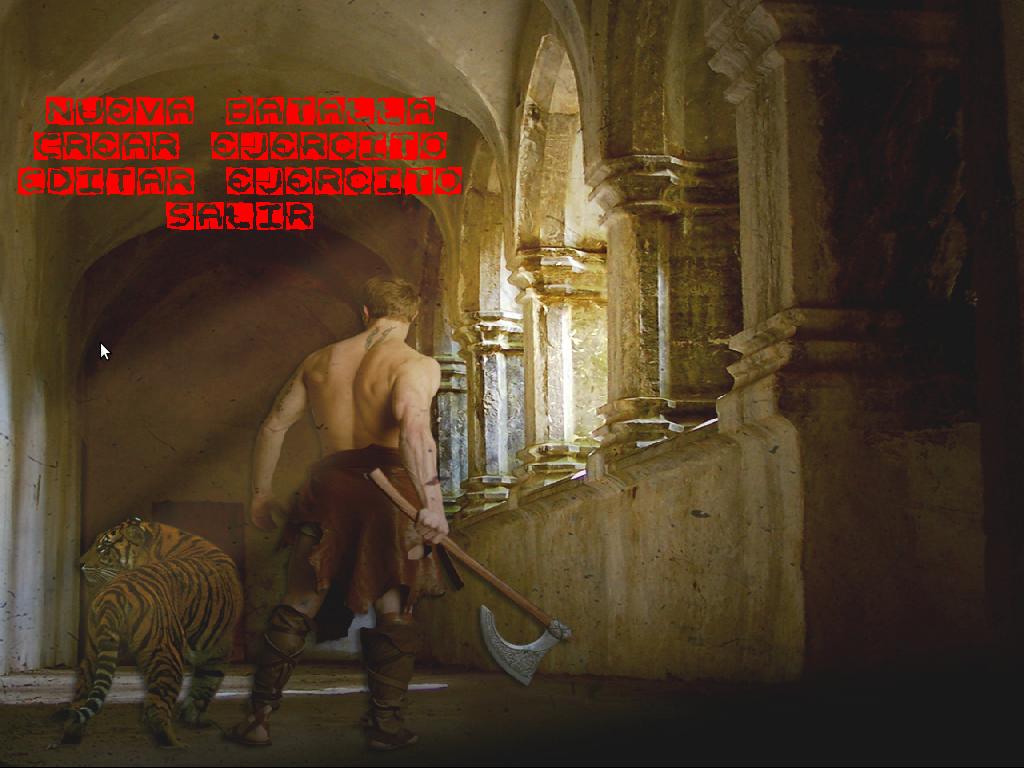
\includegraphics[scale=.4]{./imagenes/menuprincipal.png}
\label{fig:menuprincipal}
\caption{Menú principal del juego}
\end{figure}

\subsection*{\textsc{Nueva batalla}}
Al pulsar esta opción, se nos presenta un nuevo menú contextual para
elegir los ejércitos que protagonizarán la batalla. Se deberá escoger
al primer ejército, eligiendo un ejército de la lista de ejércitos
presente en el sumario, y pulsando la flecha que apunta a la primera
caja de texto, y al segundo ejército haciendo lo propio para la
segunda.

\begin{figure}[h]
\centering
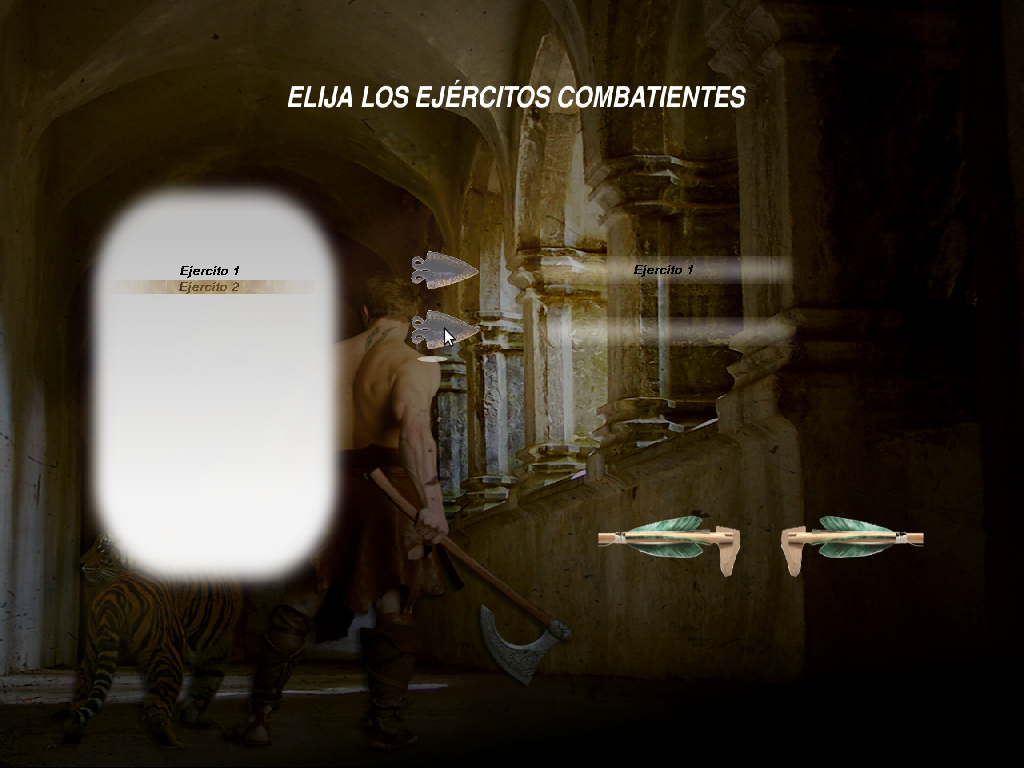
\includegraphics[scale=.4]{./imagenes/comenzarcombate.png}
\label{fig:comenzarcombate}
\caption{Menú de comienzo de batalla}
\end{figure}

Una vez elegidos ambos ejércitos, pulsamos la flecha que apunta a la
derecha, en la zona inferior de la pantalla, para comenzar una nueva
batalla, y se nos presenta el
escenario, con las unidades de ambos ejércitos desplegados, listo para
comenzar una batalla.

Si en vez de ir a la batalla, se desea cancelar la acción, basta
pulsar la flecha que apunta a la izquierda, en la zona inferior de la
pantalla, para regresar al menú principal.

\subsection*{\textsc{Crear ejército}}
En esta opción, se nos presenta una interfaz rica para editar nuestro
ejército con todas las herramientas necesarias para conseguirlo. Una
vez elegido un ejército, al pulsar a la flecha inferior que apunta a
la derecha, aparece una caja de texto para elegir el nombre de nuestro
ejército.

Este nombre puede estar formado por números, letras, barras bajas
(carácter '\_') y
espacios, pero no se pueden escribir ninguna otra clase de
carácteres. Una vez escrito, se vuelve a pulsar en la flecha derecha y
el ejército será añadido al sistema, y se volverá al menú
principal. Si se desea cancelar, se pulsa a la flecha izquierda y se
vuelve al menú de edición de ejércitos, con la misma configuración que
anteriormente. Ahora, si así lo deseas, puedes modificar tu ejército y
finalmente guardarlo.

Si al contrario, se desea cancelar la creación de un ejército, se
puede pulsar la flecha que apunta a la izquierda para retornar al menú
principal del juego.

\subsection*{\textsc{Editar ejército}}
Con esta opción, si se elige una unidad y se pulsa en la flecha
derecha, se llega al menú presentado en la sección anterior, salvo que
ahora se muestra en pantalla la configuración actual del ejército
elegido para la edición.

Se prosigue con en el caso anterior. Si se continúa, se puede
modificar el nombre del ejército, y luego añadir el nuevo nombre al
sistema.

\begin{figure}[h]
\centering
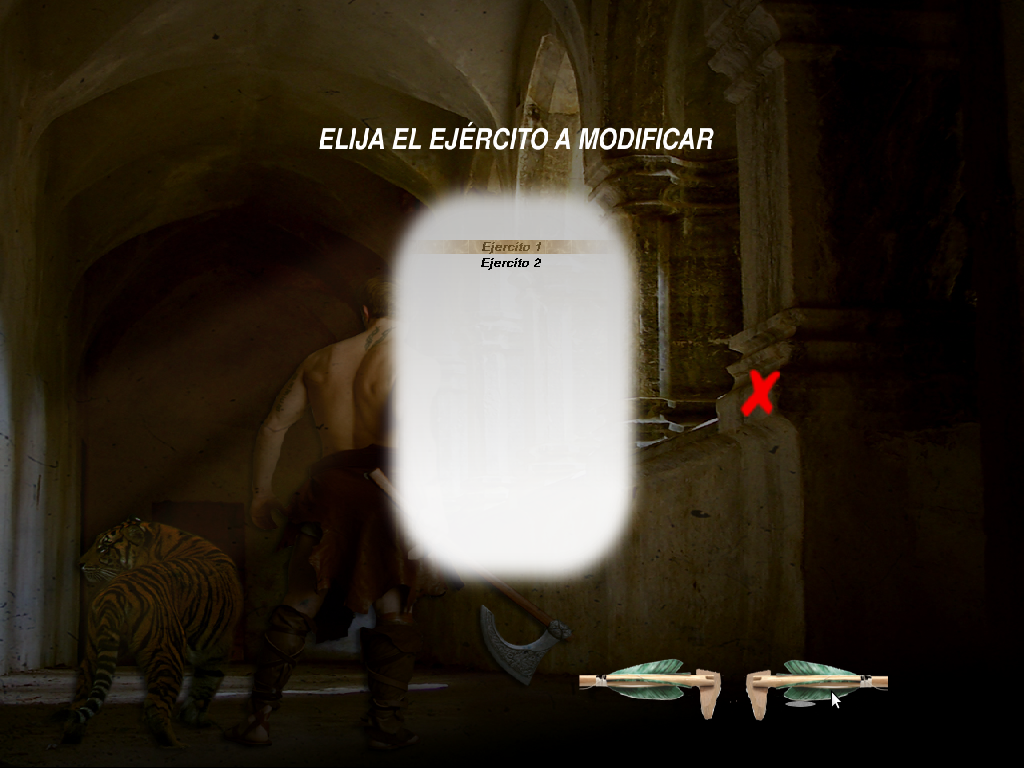
\includegraphics[scale=.4]{./imagenes/elegirejercito.png}
\label{fig:elegirejercito}
\caption{Menú de elección de ejército de edición}
\end{figure}

Con la flecha izquierda, se puede
retornar a pantallas anteriores sin deshacer los cambios.

Con la cruz roja se pueden eliminar ejército existentes, con solo
seleccionar el ejército y pulsar a continuación en la cruz roja.

\subsection*{\textsc{Salir}}
Con esta opción se abandona \gom y se cierra el programa.

\section*{Menú de edición de ejército}
Aquí se explica mas concisamente los elementos involucrados en el menú
de edición de un ejército.

Se pueden observar concretamente 5 secciones:
\begin{itemize}
\item El menú desplegable de elección de raza, en la parte
  superior izquierda de la pantalla.
\item La lista de unidades de raza, justo debajo del menú desplegable
  de elección de raza.
\item El sumario del ejército, en la parte medio e inferior derecha de
  la pantalla.
\item Los campos de edición de unidad, justo encima del sumario de
  unidades.
\item Las flechas de abandono y salvado del ejército, en la parte inferior
  derecha de la pantalla.
\end{itemize}

\begin{figure}[h]
\centering
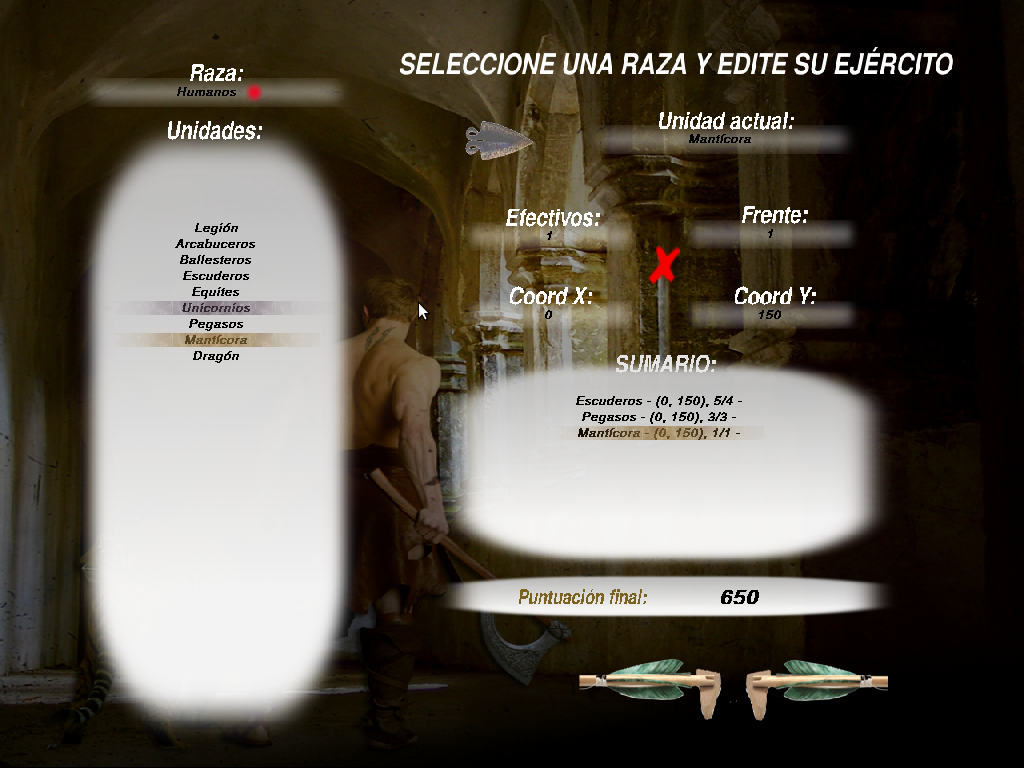
\includegraphics[scale=.4]{./imagenes/configurarejercito.png}
\label{fig:confejercito}
\caption{Menú de edición de ejército}
\end{figure}

\subsection*{Menú desplegable de elección de raza}
Es el recuadro titulado con el nombre \textsc{\textit{``Raza''}}. Si
se coloca el ratón encima del botón rojo, ese se ilumina, y si se
pulsa se despliega un menú en donde se puede elegir la raza de tu
ejército.

Una vez elegido, en la lista de unidades se muestran todas las
unidades disponibles para la raza elegida, que podrán seleccionarse
para añadirlas al sumario del ejército.

Si ya existía un ejército configurado, al cambiar de raza, toda la
información de la edición del ejército se borrará. Si se pulsa la
flecha de abandono, no se grabarán los cambios, y el ejército, si
existía, mantendrá su configuración original antes de la edición.

\subsubsection*{Lista de unidades de raza}
En esta lista se muestran todas las unidades disponibles para el
ejército elegido actualmente. Si se selecciona una unidad y se pulsa
la flecha situada mas arriba, esta unidad se añadirá al sumario de
unidades, y aparecerán los valores por defecto de la unidad en los
campos de edición de unidades, que podrán ser modificador inmediatamente.

Una vez pulsada una unidad, se podrán añadir tantas veces como se
desee con solo pulsar repetidas veces dicha flecha, con lo cual se
enriquecerá el sumario y aumentará el tamaño en puntos y el número de
unidades de tu ejército.

\subsubsection*{Sumario del ejército}
El sumario del ejército es el panel que refleja la lista de todas las
unidades, junto con su configuración, que conforman al ejército
actual. Entre la configuración del ejército se incluye su posición de
despliegue, su frente y el número de efectivos de la unidad. Toda esta
configuración es editable en los campos de edición de unidad.

El formato de la presentación de cada ítem en el sumario es la
siguiente:

\begin{center}
\textit{nombre de la unidad -(coordenada x, coordenada y) efectivos/frente-}
\end{center}

Si se desea eliminar una unidad del sumario, basta con seleccionarla y
pulsar la cruz roja, y ésta desaparecerá del sumario y no pertenecerá
al ejército final. Si se desea editar la configuración de la unidad,
basta con seleccionarla y modificar los campos de edición de la
unidad.

Si el número de unidades es mayor que la disponible por el tamaño del
cuadro del sumario, aparecerá unas flechas que permiten subir y bajar
en la lista de unidades.

Si existen unidades que se pisan (es decir, que la distancia entre
ellas no respetan la distancia de separación exigida en \gomf), o
unidades que en su despliegue aparecerían fuera total o parcialmente
del campo de batalla, al intentar continuar para grabar el ejército,
se mostrará un símbolo de error (una cruz roja) a la derecha de los
elementos conflictivos. El usuario deberá ver a las unidades y
observar el error, seleccionar a la unidad, y corregir los posibles errores.

Justo abajo del sumario se muestra un campo llamado \emph{puntuación
  final} con la suma total en
puntos de las unidades elegidas. Es decir, el coste total del ejército.

\subsubsection*{Campos de edición de unidad}
Los campos de edición de unidad son cuatro:

\begin{itemize}
\item Coordenada x
\item Coordenada y
\item Efectivos
\item Frente
\end{itemize}

\paragraph{Coordenada x}
Almacena la coordenada x de la unidad para la confección de su
despliegue. Un valor muy alto de la coordenada x puede hacer que la
unidad salga fuera de la zona de despliegue. En estos casos, no se
podrá grabar el ejército y se indicará en el sumario la unidad que
provoca el error. Lo mismo ocurre si se violan cualquiera de las
restricciones del despliegue de un ejército.

No se permiten introducir números negativos.

\paragraph{Coordenada y}
Al igual que en el párrafo anterior, almacena la coordenada y para la
confección del despliegue de la unidad seleccionada en el sumario. Si
el valor de la coordenada y es muy alta, o en general, esa unidad
provoca un despliegue incorrecto, el sistema
indicará que la unidad provoca un error.

No se permiten introducir números negativos.

\paragraph{Efectivos}
Es el número de efectivos de la unidad. Por defecto, aparece el número
mínimo de efectivos que la descripción de la unidad permite. Si se
introduce un número menor, se retorna el valor al valor por
defecto. Si se escribe un número mayor al número máximo de efectivos
de la unidad, se configura con el valor máximo de efectivos de la
unidad. No se permiten introducir números negativos.

Si el tamaño de la unidad hace que el despliegue sea inválido, se
indica que la unidad provoca error al intentar grabar los cambios en
el ejército.

\paragraph{Frente}
Análogamente a la cantidad de efectivos, por defecto aparece el número
mínimo de frente de la unidad, que es 4; o menos si el número mínimo
de efectivos de la unidad es también menor que 4. En éste caso
aparecerá este último número por defecto.

Si se introduce un número menor, se retorna al valor por defecto de
esa unidad.

No hay límite acerca del tamaño del frente, salvo si un frente
demasiado ancho provoca un despliegue incorrecto. En este caso, se
indicará que la unidad provoca un error al intentar grabar los cambios
del ejército.

No se permiten introducir números negativos.

\section*{Pantalla de batalla}
Cuando el usuario elige la primera opción del menú, la de
\textsc{\textit{Nueva batalla}}, y se elijan a los ejércitos y de
comienzo a la batalla, aparecerá una pantalla divida en tres
secciones:

\begin{itemize}
\item Zona de iconos
\item Campo de batalla
\item Zona de descripciones
\end{itemize}

\begin{figure}[h]
\centering
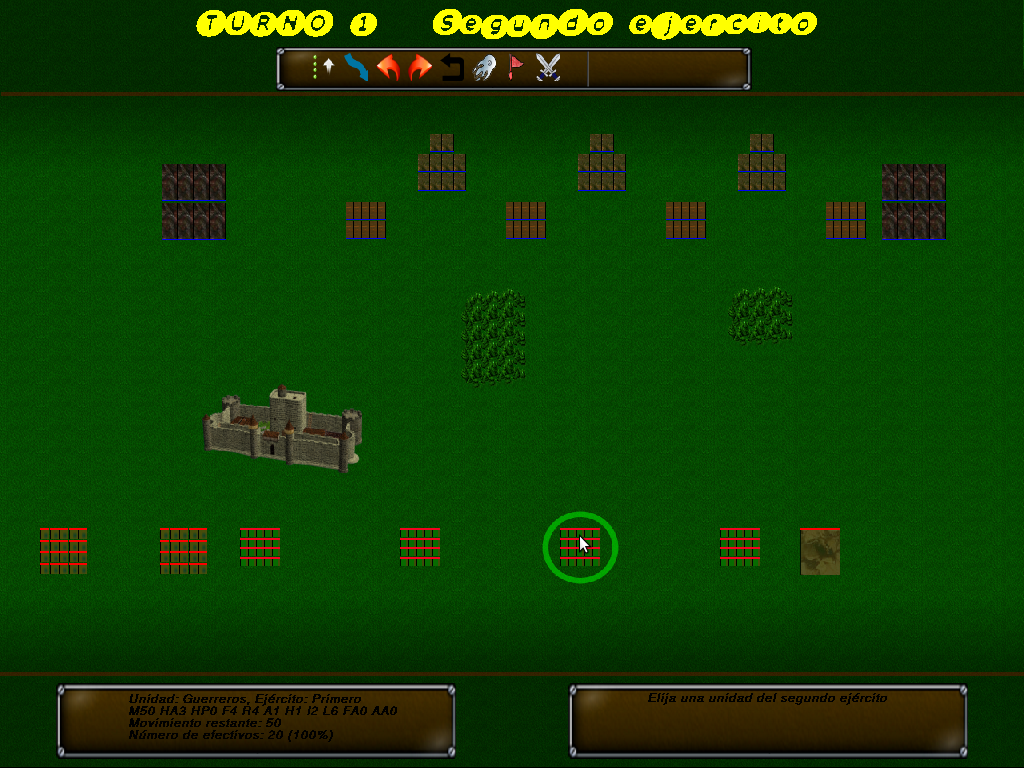
\includegraphics[scale=.4]{./imagenes/campobatalla.png}
\label{fig:campobatalla}
\caption{Campo de batalla}
\end{figure}

Cada una de éstas secciones de la pantalla de batalla se comentan a continuación.

\subsection*{Zona de iconos}
La zona de iconos reside en la parte superior del campo, en la zona
verde sombreada, justo encima de la franja roja transparente
superior.

Posee dos partes diferenciadas, el título de turno, y el menú de
iconos. El título de turno es sencillamente una descripción textual
del turno o situación actual: \textit{\textsc{Ejércitos desplegados}},
\textit{\textsc{Turno 1 Ejército primero}}, \textit{\textsc{Turno 1
    Ejército segundo}}, \textit{\textsc{Turno 2 Ejército primero}},
etc.

La zona de iconos es donde propiamente están todos los iconos que
permiten realizar todas las acciones del juego. Se diferencias dos
partes separadas por una barra, dentro del marco donde residen los
iconos.

En la primera parte, o parte izquierda, están todos los iconos que
pueden usarse ahora mismo para realizar acciones. Aparecen centrados
en su zona correspondiente. En la segunda, o parte derecha, aparecen
apiladas a la izquierda (como si de una secuencia se tratara), todos
los iconos que están activos pero no disponibles, esto es, de tareas
pendientes.

Si se pulsa en cualquiera de los iconos de la \textit{primera
  categoría}, se ejecuta su acción inmeditamente. Si se pulsa en
cualquiera de los iconos de la segunda, no se realiza ninguna acción
en el campo de batalla.

\subsection*{Zona de descripciones}
La zona de descripciones distingue dos partes, un primer marco, o
marco izquierdo, y un segundo marco, o marco derecho.

En el marco izquierdo, se muestra información de los elementos en los
que esté situado actualmente el ratón.

Si el ratón está situado en la zona de iconos, justo encima de alguno,
se muestra en este marco la descripción de la utilidad de dicho icono.

Si el ratón está situado encima de una unidad del campo de batalla, se
muestra, y en este orden:

\begin{itemize}
\item el nombre de la unidad.
\item el ejército al que pertenece a la unidad.
\item el perfil de atributos de la unidad.
\item la cantidad de movimiento restante de la unidad.
\item el número de efectivos actual de la unidad, junto al porcentaje
  de efectivos actuales respecto al original.
\item una descripción del estado especial de la unidad: huyendo,
  marchando o combatiendo. Si la unidad no está en ninguna de estas
  tres situaciones, no se mostrará nada acerca del estado de la unidad
  (su estado es el normal y predeterminado).
\end{itemize}

Si el usuario intenta realizar una acción no permitida, se muestra, en
el segundo panel, una breve descripción del motivo del error.

\subsection*{Campo de batalla}
El campo de batalla es el delimitado por arriba y por abajo por una
línea semitransparente de color rojo, que marca, junto con los bordes
de la pantalla, el límite del campo de batalla.

Dentro se sitúan todas las unidades presentes en la partida. Si una
unidad se retira de la batalla, su unidad no volverá a aparecer en el
campo de batalla.

La zona de despliegue del jugador uno es la parte inferior del campo
de batalla, y ocupa el primer 25\%, en dirección vertical, del campo
de batalla. La zona de despliegue del jugador dos es el 25\% superior
del campo de batalla.

\subsubsection*{Unidades}
Las unidades aparecerán como un conjunto homogeneo de efectivos, donde
cada efectivo es representado como un cuadrito con un dibujo
decorativo que distingue a los efectivos de una unidad de las
restantes. No existirán dos unidades distintas que tengan un igual
dibujo para sus efectivos.

A cada ejército le corresponderá un color. Al primero le corresponderá
el color rojo. Al segundo, el color azul. Los efectivos tienen
coloreado con el color de su equipo su propio frente, y además, cuando
se pasa el ratón por encima de una unidad, la circunferencia que
muestra la unidad apuntada por el ratón tendrá también el color de la
equipo de la unidad.

\subsubsection*{Escenografía}
El escenario posee un número aleatorio de elementos de escenografía
repartidos por el escenario, pero nunca en las zonas de despliegue ni
en sus cercanías.

En el reglamento de \gom se permite una total libertad a la hora de
tratar y colocar elementos de escenografía en el escenario.

En \gom se ha establecido la escenografía del juego de la siguiente
forma:
\begin{itemize}
\item Se divide el campo de batalla (excluyendo la zona de despliegue
  y el espacio de separación impuesto por el reglamento de \gomf) en 2
  ó 3 secciones. Esta cantidad se selecciona al azar.
\item De entre éstas 2 o 3 secciones, a una le corresponderá un
  edificio. A las restantes bosques.
\item La posición del edificio será determinada al azar dentro de su
  sección de campo correspondiente.
\item La posición de cada bosques también será determinada al azar
  dentro de su sección de campo correspondiente, así como el tamaño
  del mismo, que nunca corresponderá a un área mayor al 10\% de dicha
  sección.
\end{itemize}

Los elementos de escenografía, además, también imponen respetar un
espacio igual al espacio de unidades entre ellas, además de ser terreno impasable.

\subsubsection*{Transcurso de la batalla}
Al comenzar la batalla, las unidades aparecerán desplegadas en su
correspondiente lugar de acuerdo a la configuración del ejército
diseñado. A partir de entonces, los jugadores podrán, haciendo uso de
los iconos, y interactuando con el sistema, ejecutar todas las
acciones deseadas por el usuario, así como las requeridas por \gomf.

Una unidad siempre podrá seleccionarse con solo pulsar con el ratón
encima de ella. Al hacerlo, se mantenderá una circunferencia de color verde indicando que la unidad ha sido
seleccionada. Si se ejecuta alguna acción, y ésta se aplica a una
unidad (por ejemplo, un giro), la acción se ejecutará sobre esa
unidad. Si la acción se aplica a una unidad, y no hay ninguna
seleccionada, o hay seleccionada una del bando contrario al turno en
curso, se indica un mensaje de error en el marco derecho de la zona de
descripción..

Las acciones que necesiten información por parte del usuario son
pedidas dinámicamente en el campo de batalla. Por ejemplo, si una
unidad desea realizar un desplazamiento, se mostrará una zona
sombreada correspondiente al área dentro del cual la unidad podrá
desplazarse.

Apuntando con el ratón dentro de dicho área, se mostrará un cuadro
ficticio indicando la posición final de la unidad. Al pulsar sobre una
posición dentro del área, la unidad se mueve definitivamente a esa
posición.

Este comportamiento es igual en todas las acciones que
requieren información por parte del usuario, como el desplazamiento a
realizar, en el caso anterior. Se dispondrá de unos indicativos
visuales a las que el usuario deberá responder.

La batalla finaliza al llevar 6 turnos de juego, o al indicarlo el
usuario con el icono correspondiente.

\subsubsection*{Pantalla de resultado del combate}
Al finalizar la batalla, se muestra un menú que indica al ganador de
la batalla y la distribución en puntos de la misma.

Se divide en 4 partes:
\begin{itemize}
\item Descripción de los puntos del jugador 1.
\item Descripción de los puntos del jugador 2.
\item Sumario comparativo.
\item Ganador.
\end{itemize}

\begin{figure}[h]
\centering
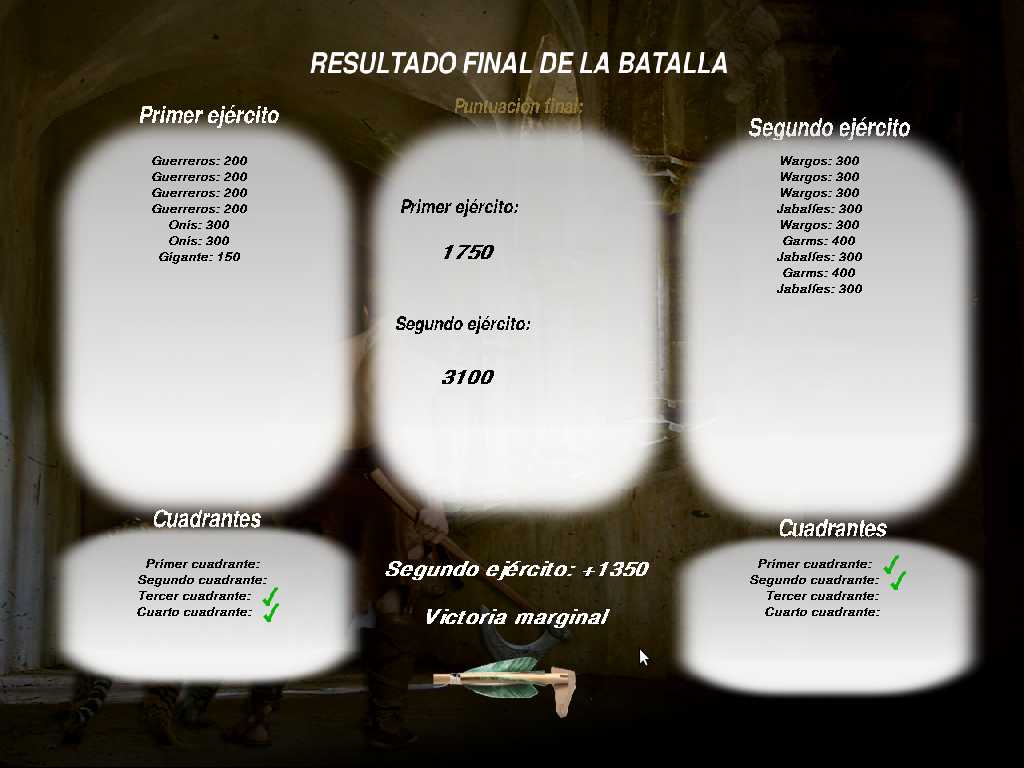
\includegraphics[scale=.4]{./imagenes/resultado.png}
\label{fig:imgresultado}
\caption{Menú de resultado de la batalla}
\end{figure}


\paragraph{Descripción de los puntos del jugador 1 y 2}
Son dos secciones que se encuentran, respectivamente, a la izquierda y
a la derecha de la pantalla para los jugadores 1 y 2. En ambos lados,
existe una parte superior que muestra las unidades, y una parte
inferior que muestra los cuadrantes.

En la descripción de las unidades, se coloca la puntuación obtenida
por ella tal y como expone el reglamento de \gom en su sección
correspondiente al resultado de una batalla.

En la descripción a los cuadrantes, se muestra una lista de cuatro
cuadrante y una señal de acierto para los cuadrantes que hayan caido
en posesión del ejército correspondiente.

\paragraph{Sumario comparativo}
Es la zona que está en el centro de este menú, la más alta. Se muestra
la ponderación total en puntos de ambas unidades, es decir, la suma de
los puntos obtenidos por unidades y por cuadrantes.

\paragraph{Ganador}
Se muestra el nombre del jugador ganador, así como el tipo de
victoria: \emph{masacre}, \emph{victoria decisiva} o \emph{victoria
  marginal}.

Si la partida acaba en \emph{empate}, evidentemente no habrá ningún
ejército ganador que mostrar y solo se indicará que la situación final
de la pantalla ha sido un empate.

\nocite{pressman}
\nocite{laur04}
\nocite{raym01}
\nocite{stal04}
\nocite{mitt04}
\nocite{sdlweb}
\nocite{sdlosluca}
\nocite{cppref}
\nocite{warh}

\clearpage
\phantomsection
\addcontentsline{toc}{chapter}{Bibliografía y referencias}
\bibliographystyle{plain}
\bibliography{bibliografia.bib}

% This is set up to run with pdflatex.
%---------The file header---------------------------------------------
%---------------------------------------------------------------------
\chapter*{\rlap{GNU Free Documentation License}}
\phantomsection  % so hyperref creates bookmarks
\addcontentsline{toc}{chapter}{GNU Free Documentation License}
%\label{label_fdl}

 \begin{center}

       Version 1.3, 3 November 2008


 Copyright \copyright{} 2000, 2001, 2002, 2007, 2008  Free Software Foundation, Inc.
 
 \bigskip
 
     <http://fsf.org/>
  
 \bigskip
 
 Everyone is permitted to copy and distribute verbatim copies
 of this license document, but changing it is not allowed.
\end{center}


\begin{center}
{\bf\large Preamble}
\end{center}

The purpose of this License is to make a manual, textbook, or other
functional and useful document ``free'' in the sense of freedom: to
assure everyone the effective freedom to copy and redistribute it,
with or without modifying it, either commercially or noncommercially.
Secondarily, this License preserves for the author and publisher a way
to get credit for their work, while not being considered responsible
for modifications made by others.

This License is a kind of ``copyleft'', which means that derivative
works of the document must themselves be free in the same sense.  It
complements the GNU General Public License, which is a copyleft
license designed for free software.

We have designed this License in order to use it for manuals for free
software, because free software needs free documentation: a free
program should come with manuals providing the same freedoms that the
software does.  But this License is not limited to software manuals;
it can be used for any textual work, regardless of subject matter or
whether it is published as a printed book.  We recommend this License
principally for works whose purpose is instruction or reference.


\begin{center}
{\Large\bf 1. APPLICABILITY AND DEFINITIONS\par}
\phantomsection
\addcontentsline{toc}{section}{1. APPLICABILITY AND DEFINITIONS}
\end{center}

This License applies to any manual or other work, in any medium, that
contains a notice placed by the copyright holder saying it can be
distributed under the terms of this License.  Such a notice grants a
world-wide, royalty-free license, unlimited in duration, to use that
work under the conditions stated herein.  The ``\textbf{Document}'', below,
refers to any such manual or work.  Any member of the public is a
licensee, and is addressed as ``\textbf{you}''.  You accept the license if you
copy, modify or distribute the work in a way requiring permission
under copyright law.

A ``\textbf{Modified Version}'' of the Document means any work containing the
Document or a portion of it, either copied verbatim, or with
modifications and/or translated into another language.

A ``\textbf{Secondary Section}'' is a named appendix or a front-matter section of
the Document that deals exclusively with the relationship of the
publishers or authors of the Document to the Document's overall subject
(or to related matters) and contains nothing that could fall directly
within that overall subject.  (Thus, if the Document is in part a
textbook of mathematics, a Secondary Section may not explain any
mathematics.)  The relationship could be a matter of historical
connection with the subject or with related matters, or of legal,
commercial, philosophical, ethical or political position regarding
them.

The ``\textbf{Invariant Sections}'' are certain Secondary Sections whose titles
are designated, as being those of Invariant Sections, in the notice
that says that the Document is released under this License.  If a
section does not fit the above definition of Secondary then it is not
allowed to be designated as Invariant.  The Document may contain zero
Invariant Sections.  If the Document does not identify any Invariant
Sections then there are none.

The ``\textbf{Cover Texts}'' are certain short passages of text that are listed,
as Front-Cover Texts or Back-Cover Texts, in the notice that says that
the Document is released under this License.  A Front-Cover Text may
be at most 5 words, and a Back-Cover Text may be at most 25 words.

A ``\textbf{Transparent}'' copy of the Document means a machine-readable copy,
represented in a format whose specification is available to the
general public, that is suitable for revising the document
straightforwardly with generic text editors or (for images composed of
pixels) generic paint programs or (for drawings) some widely available
drawing editor, and that is suitable for input to text formatters or
for automatic translation to a variety of formats suitable for input
to text formatters.  A copy made in an otherwise Transparent file
format whose markup, or absence of markup, has been arranged to thwart
or discourage subsequent modification by readers is not Transparent.
An image format is not Transparent if used for any substantial amount
of text.  A copy that is not ``Transparent'' is called ``\textbf{Opaque}''.

Examples of suitable formats for Transparent copies include plain
ASCII without markup, Texinfo input format, LaTeX input format, SGML
or XML using a publicly available DTD, and standard-conforming simple
HTML, PostScript or PDF designed for human modification.  Examples of
transparent image formats include PNG, XCF and JPG.  Opaque formats
include proprietary formats that can be read and edited only by
proprietary word processors, SGML or XML for which the DTD and/or
processing tools are not generally available, and the
machine-generated HTML, PostScript or PDF produced by some word
processors for output purposes only.

The ``\textbf{Title Page}'' means, for a printed book, the title page itself,
plus such following pages as are needed to hold, legibly, the material
this License requires to appear in the title page.  For works in
formats which do not have any title page as such, ``Title Page'' means
the text near the most prominent appearance of the work's title,
preceding the beginning of the body of the text.

The ``\textbf{publisher}'' means any person or entity that distributes
copies of the Document to the public.

A section ``\textbf{Entitled XYZ}'' means a named subunit of the Document whose
title either is precisely XYZ or contains XYZ in parentheses following
text that translates XYZ in another language.  (Here XYZ stands for a
specific section name mentioned below, such as ``\textbf{Acknowledgements}'',
``\textbf{Dedications}'', ``\textbf{Endorsements}'', or ``\textbf{History}''.)  
To ``\textbf{Preserve the Title}''
of such a section when you modify the Document means that it remains a
section ``Entitled XYZ'' according to this definition.

The Document may include Warranty Disclaimers next to the notice which
states that this License applies to the Document.  These Warranty
Disclaimers are considered to be included by reference in this
License, but only as regards disclaiming warranties: any other
implication that these Warranty Disclaimers may have is void and has
no effect on the meaning of this License.


\begin{center}
{\Large\bf 2. VERBATIM COPYING\par}
\phantomsection
\addcontentsline{toc}{section}{2. VERBATIM COPYING}
\end{center}

You may copy and distribute the Document in any medium, either
commercially or noncommercially, provided that this License, the
copyright notices, and the license notice saying this License applies
to the Document are reproduced in all copies, and that you add no other
conditions whatsoever to those of this License.  You may not use
technical measures to obstruct or control the reading or further
copying of the copies you make or distribute.  However, you may accept
compensation in exchange for copies.  If you distribute a large enough
number of copies you must also follow the conditions in section~3.

You may also lend copies, under the same conditions stated above, and
you may publicly display copies.


\begin{center}
{\Large\bf 3. COPYING IN QUANTITY\par}
\phantomsection
\addcontentsline{toc}{section}{3. COPYING IN QUANTITY}
\end{center}


If you publish printed copies (or copies in media that commonly have
printed covers) of the Document, numbering more than 100, and the
Document's license notice requires Cover Texts, you must enclose the
copies in covers that carry, clearly and legibly, all these Cover
Texts: Front-Cover Texts on the front cover, and Back-Cover Texts on
the back cover.  Both covers must also clearly and legibly identify
you as the publisher of these copies.  The front cover must present
the full title with all words of the title equally prominent and
visible.  You may add other material on the covers in addition.
Copying with changes limited to the covers, as long as they preserve
the title of the Document and satisfy these conditions, can be treated
as verbatim copying in other respects.

If the required texts for either cover are too voluminous to fit
legibly, you should put the first ones listed (as many as fit
reasonably) on the actual cover, and continue the rest onto adjacent
pages.

If you publish or distribute Opaque copies of the Document numbering
more than 100, you must either include a machine-readable Transparent
copy along with each Opaque copy, or state in or with each Opaque copy
a computer-network location from which the general network-using
public has access to download using public-standard network protocols
a complete Transparent copy of the Document, free of added material.
If you use the latter option, you must take reasonably prudent steps,
when you begin distribution of Opaque copies in quantity, to ensure
that this Transparent copy will remain thus accessible at the stated
location until at least one year after the last time you distribute an
Opaque copy (directly or through your agents or retailers) of that
edition to the public.

It is requested, but not required, that you contact the authors of the
Document well before redistributing any large number of copies, to give
them a chance to provide you with an updated version of the Document.


\begin{center}
{\Large\bf 4. MODIFICATIONS\par}
\phantomsection
\addcontentsline{toc}{section}{4. MODIFICATIONS}
\end{center}

You may copy and distribute a Modified Version of the Document under
the conditions of sections 2 and 3 above, provided that you release
the Modified Version under precisely this License, with the Modified
Version filling the role of the Document, thus licensing distribution
and modification of the Modified Version to whoever possesses a copy
of it.  In addition, you must do these things in the Modified Version:

\begin{itemize}
\item[A.] 
   Use in the Title Page (and on the covers, if any) a title distinct
   from that of the Document, and from those of previous versions
   (which should, if there were any, be listed in the History section
   of the Document).  You may use the same title as a previous version
   if the original publisher of that version gives permission.
   
\item[B.]
   List on the Title Page, as authors, one or more persons or entities
   responsible for authorship of the modifications in the Modified
   Version, together with at least five of the principal authors of the
   Document (all of its principal authors, if it has fewer than five),
   unless they release you from this requirement.
   
\item[C.]
   State on the Title page the name of the publisher of the
   Modified Version, as the publisher.
   
\item[D.]
   Preserve all the copyright notices of the Document.
   
\item[E.]
   Add an appropriate copyright notice for your modifications
   adjacent to the other copyright notices.
   
\item[F.]
   Include, immediately after the copyright notices, a license notice
   giving the public permission to use the Modified Version under the
   terms of this License, in the form shown in the Addendum below.
   
\item[G.]
   Preserve in that license notice the full lists of Invariant Sections
   and required Cover Texts given in the Document's license notice.
   
\item[H.]
   Include an unaltered copy of this License.
   
\item[I.]
   Preserve the section Entitled ``History'', Preserve its Title, and add
   to it an item stating at least the title, year, new authors, and
   publisher of the Modified Version as given on the Title Page.  If
   there is no section Entitled ``History'' in the Document, create one
   stating the title, year, authors, and publisher of the Document as
   given on its Title Page, then add an item describing the Modified
   Version as stated in the previous sentence.
   
\item[J.]
   Preserve the network location, if any, given in the Document for
   public access to a Transparent copy of the Document, and likewise
   the network locations given in the Document for previous versions
   it was based on.  These may be placed in the ``History'' section.
   You may omit a network location for a work that was published at
   least four years before the Document itself, or if the original
   publisher of the version it refers to gives permission.
   
\item[K.]
   For any section Entitled ``Acknowledgements'' or ``Dedications'',
   Preserve the Title of the section, and preserve in the section all
   the substance and tone of each of the contributor acknowledgements
   and/or dedications given therein.
   
\item[L.]
   Preserve all the Invariant Sections of the Document,
   unaltered in their text and in their titles.  Section numbers
   or the equivalent are not considered part of the section titles.
   
\item[M.]
   Delete any section Entitled ``Endorsements''.  Such a section
   may not be included in the Modified Version.
   
\item[N.]
   Do not retitle any existing section to be Entitled ``Endorsements''
   or to conflict in title with any Invariant Section.
   
\item[O.]
   Preserve any Warranty Disclaimers.
\end{itemize}

If the Modified Version includes new front-matter sections or
appendices that qualify as Secondary Sections and contain no material
copied from the Document, you may at your option designate some or all
of these sections as invariant.  To do this, add their titles to the
list of Invariant Sections in the Modified Version's license notice.
These titles must be distinct from any other section titles.

You may add a section Entitled ``Endorsements'', provided it contains
nothing but endorsements of your Modified Version by various
parties---for example, statements of peer review or that the text has
been approved by an organization as the authoritative definition of a
standard.

You may add a passage of up to five words as a Front-Cover Text, and a
passage of up to 25 words as a Back-Cover Text, to the end of the list
of Cover Texts in the Modified Version.  Only one passage of
Front-Cover Text and one of Back-Cover Text may be added by (or
through arrangements made by) any one entity.  If the Document already
includes a cover text for the same cover, previously added by you or
by arrangement made by the same entity you are acting on behalf of,
you may not add another; but you may replace the old one, on explicit
permission from the previous publisher that added the old one.

The author(s) and publisher(s) of the Document do not by this License
give permission to use their names for publicity for or to assert or
imply endorsement of any Modified Version.


\begin{center}
{\Large\bf 5. COMBINING DOCUMENTS\par}
\phantomsection
\addcontentsline{toc}{section}{5. COMBINING DOCUMENTS}
\end{center}


You may combine the Document with other documents released under this
License, under the terms defined in section~4 above for modified
versions, provided that you include in the combination all of the
Invariant Sections of all of the original documents, unmodified, and
list them all as Invariant Sections of your combined work in its
license notice, and that you preserve all their Warranty Disclaimers.

The combined work need only contain one copy of this License, and
multiple identical Invariant Sections may be replaced with a single
copy.  If there are multiple Invariant Sections with the same name but
different contents, make the title of each such section unique by
adding at the end of it, in parentheses, the name of the original
author or publisher of that section if known, or else a unique number.
Make the same adjustment to the section titles in the list of
Invariant Sections in the license notice of the combined work.

In the combination, you must combine any sections Entitled ``History''
in the various original documents, forming one section Entitled
``History''; likewise combine any sections Entitled ``Acknowledgements'',
and any sections Entitled ``Dedications''.  You must delete all sections
Entitled ``Endorsements''.

\begin{center}
{\Large\bf 6. COLLECTIONS OF DOCUMENTS\par}
\phantomsection
\addcontentsline{toc}{section}{6. COLLECTIONS OF DOCUMENTS}
\end{center}

You may make a collection consisting of the Document and other documents
released under this License, and replace the individual copies of this
License in the various documents with a single copy that is included in
the collection, provided that you follow the rules of this License for
verbatim copying of each of the documents in all other respects.

You may extract a single document from such a collection, and distribute
it individually under this License, provided you insert a copy of this
License into the extracted document, and follow this License in all
other respects regarding verbatim copying of that document.


\begin{center}
{\Large\bf 7. AGGREGATION WITH INDEPENDENT WORKS\par}
\phantomsection
\addcontentsline{toc}{section}{7. AGGREGATION WITH INDEPENDENT WORKS}
\end{center}


A compilation of the Document or its derivatives with other separate
and independent documents or works, in or on a volume of a storage or
distribution medium, is called an ``aggregate'' if the copyright
resulting from the compilation is not used to limit the legal rights
of the compilation's users beyond what the individual works permit.
When the Document is included in an aggregate, this License does not
apply to the other works in the aggregate which are not themselves
derivative works of the Document.

If the Cover Text requirement of section~3 is applicable to these
copies of the Document, then if the Document is less than one half of
the entire aggregate, the Document's Cover Texts may be placed on
covers that bracket the Document within the aggregate, or the
electronic equivalent of covers if the Document is in electronic form.
Otherwise they must appear on printed covers that bracket the whole
aggregate.


\begin{center}
{\Large\bf 8. TRANSLATION\par}
\phantomsection
\addcontentsline{toc}{section}{8. TRANSLATION}
\end{center}


Translation is considered a kind of modification, so you may
distribute translations of the Document under the terms of section~4.
Replacing Invariant Sections with translations requires special
permission from their copyright holders, but you may include
translations of some or all Invariant Sections in addition to the
original versions of these Invariant Sections.  You may include a
translation of this License, and all the license notices in the
Document, and any Warranty Disclaimers, provided that you also include
the original English version of this License and the original versions
of those notices and disclaimers.  In case of a disagreement between
the translation and the original version of this License or a notice
or disclaimer, the original version will prevail.

If a section in the Document is Entitled ``Acknowledgements'',
``Dedications'', or ``History'', the requirement (section~4) to Preserve
its Title (section~1) will typically require changing the actual
title.


\begin{center}
{\Large\bf 9. TERMINATION\par}
\phantomsection
\addcontentsline{toc}{section}{9. TERMINATION}
\end{center}


You may not copy, modify, sublicense, or distribute the Document
except as expressly provided under this License.  Any attempt
otherwise to copy, modify, sublicense, or distribute it is void, and
will automatically terminate your rights under this License.

However, if you cease all violation of this License, then your license
from a particular copyright holder is reinstated (a) provisionally,
unless and until the copyright holder explicitly and finally
terminates your license, and (b) permanently, if the copyright holder
fails to notify you of the violation by some reasonable means prior to
60 days after the cessation.

Moreover, your license from a particular copyright holder is
reinstated permanently if the copyright holder notifies you of the
violation by some reasonable means, this is the first time you have
received notice of violation of this License (for any work) from that
copyright holder, and you cure the violation prior to 30 days after
your receipt of the notice.

Termination of your rights under this section does not terminate the
licenses of parties who have received copies or rights from you under
this License.  If your rights have been terminated and not permanently
reinstated, receipt of a copy of some or all of the same material does
not give you any rights to use it.


\begin{center}
{\Large\bf 10. FUTURE REVISIONS OF THIS LICENSE\par}
\phantomsection
\addcontentsline{toc}{section}{10. FUTURE REVISIONS OF THIS LICENSE}
\end{center}


The Free Software Foundation may publish new, revised versions
of the GNU Free Documentation License from time to time.  Such new
versions will be similar in spirit to the present version, but may
differ in detail to address new problems or concerns.  See
http://www.gnu.org/copyleft/.

Each version of the License is given a distinguishing version number.
If the Document specifies that a particular numbered version of this
License ``or any later version'' applies to it, you have the option of
following the terms and conditions either of that specified version or
of any later version that has been published (not as a draft) by the
Free Software Foundation.  If the Document does not specify a version
number of this License, you may choose any version ever published (not
as a draft) by the Free Software Foundation.  If the Document
specifies that a proxy can decide which future versions of this
License can be used, that proxy's public statement of acceptance of a
version permanently authorizes you to choose that version for the
Document.


\begin{center}
{\Large\bf 11. RELICENSING\par}
\phantomsection
\addcontentsline{toc}{section}{11. RELICENSING}
\end{center}


``Massive Multiauthor Collaboration Site'' (or ``MMC Site'') means any
World Wide Web server that publishes copyrightable works and also
provides prominent facilities for anybody to edit those works.  A
public wiki that anybody can edit is an example of such a server.  A
``Massive Multiauthor Collaboration'' (or ``MMC'') contained in the
site means any set of copyrightable works thus published on the MMC
site.

``CC-BY-SA'' means the Creative Commons Attribution-Share Alike 3.0
license published by Creative Commons Corporation, a not-for-profit
corporation with a principal place of business in San Francisco,
California, as well as future copyleft versions of that license
published by that same organization.

``Incorporate'' means to publish or republish a Document, in whole or
in part, as part of another Document.

An MMC is ``eligible for relicensing'' if it is licensed under this
License, and if all works that were first published under this License
somewhere other than this MMC, and subsequently incorporated in whole
or in part into the MMC, (1) had no cover texts or invariant sections,
and (2) were thus incorporated prior to November 1, 2008.

The operator of an MMC Site may republish an MMC contained in the site
under CC-BY-SA on the same site at any time before August 1, 2009,
provided the MMC is eligible for relicensing.


\begin{center}
{\Large\bf ADDENDUM: How to use this License for your documents\par}
\phantomsection
\addcontentsline{toc}{section}{ADDENDUM: How to use this License for your documents}
\end{center}

To use this License in a document you have written, include a copy of
the License in the document and put the following copyright and
license notices just after the title page:

\bigskip
\begin{quote}
    Copyright \copyright{}  YEAR  YOUR NAME.
    Permission is granted to copy, distribute and/or modify this document
    under the terms of the GNU Free Documentation License, Version 1.3
    or any later version published by the Free Software Foundation;
    with no Invariant Sections, no Front-Cover Texts, and no Back-Cover Texts.
    A copy of the license is included in the section entitled ``GNU
    Free Documentation License''.
\end{quote}
\bigskip
    
If you have Invariant Sections, Front-Cover Texts and Back-Cover Texts,
replace the ``with \dots\ Texts.'' line with this:

\bigskip
\begin{quote}
    with the Invariant Sections being LIST THEIR TITLES, with the
    Front-Cover Texts being LIST, and with the Back-Cover Texts being LIST.
\end{quote}
\bigskip
    
If you have Invariant Sections without Cover Texts, or some other
combination of the three, merge those two alternatives to suit the
situation.

If your document contains nontrivial examples of program code, we
recommend releasing these examples in parallel under your choice of
free software license, such as the GNU General Public License,
to permit their use in free software.

%---------------------------------------------------------------------

% This is set up to run with pdflatex.
%---------The file header---------------------------------------------
%---------------------------------------------------------------------
\chapter*{\rlap{GNU General Public License}}
\phantomsection  % so hyperref creates bookmarks
\addcontentsline{toc}{chapter}{GNU General Public License}
\label{gpl}

\begin{center}
{\parindent 0in

Copyright \copyright\  2007 Free Software Foundation, Inc. \texttt{http://fsf.org/}

\bigskip
Everyone is permitted to copy and distribute verbatim copies of this

license document, but changing it is not allowed.}

\end{center}

\begin{center}
{\Large \sc Preamble}
\end{center}

The GNU General Public License is a free, copyleft license for
software and other kinds of works.

The licenses for most software and other practical works are designed
to take away your freedom to share and change the works.  By contrast,
the GNU General Public License is intended to guarantee your freedom to
share and change all versions of a program--to make sure it remains free
software for all its users.  We, the Free Software Foundation, use the
GNU General Public License for most of our software; it applies also to
any other work released this way by its authors.  You can apply it to
your programs, too.

When we speak of free software, we are referring to freedom, not
price.  Our General Public Licenses are designed to make sure that you
have the freedom to distribute copies of free software (and charge for
them if you wish), that you receive source code or can get it if you
want it, that you can change the software or use pieces of it in new
free programs, and that you know you can do these things.

To protect your rights, we need to prevent others from denying you
these rights or asking you to surrender the rights.  Therefore, you have
certain responsibilities if you distribute copies of the software, or if
you modify it: responsibilities to respect the freedom of others.

For example, if you distribute copies of such a program, whether
gratis or for a fee, you must pass on to the recipients the same
freedoms that you received.  You must make sure that they, too, receive
or can get the source code.  And you must show them these terms so they
know their rights.

Developers that use the GNU GPL protect your rights with two steps:
(1) assert copyright on the software, and (2) offer you this License
giving you legal permission to copy, distribute and/or modify it.

For the developers' and authors' protection, the GPL clearly explains
that there is no warranty for this free software.  For both users' and
authors' sake, the GPL requires that modified versions be marked as
changed, so that their problems will not be attributed erroneously to
authors of previous versions.

Some devices are designed to deny users access to install or run
modified versions of the software inside them, although the manufacturer
can do so.  This is fundamentally incompatible with the aim of
protecting users' freedom to change the software.  The systematic
pattern of such abuse occurs in the area of products for individuals to
use, which is precisely where it is most unacceptable.  Therefore, we
have designed this version of the GPL to prohibit the practice for those
products.  If such problems arise substantially in other domains, we
stand ready to extend this provision to those domains in future versions
of the GPL, as needed to protect the freedom of users.

Finally, every program is threatened constantly by software patents.
States should not allow patents to restrict development and use of
software on general-purpose computers, but in those that do, we wish to
avoid the special danger that patents applied to a free program could
make it effectively proprietary.  To prevent this, the GPL assures that
patents cannot be used to render the program non-free.

The precise terms and conditions for copying, distribution and
modification follow.

\begin{center}
{\Large \sc Terms and Conditions}
\end{center}


\begin{enumerate}

\addtocounter{enumi}{-1}

\item Definitions.

``This License'' refers to version 3 of the GNU General Public License.

``Copyright'' also means copyright-like laws that apply to other kinds of
works, such as semiconductor masks.

``The Program'' refers to any copyrightable work licensed under this
License.  Each licensee is addressed as ``you''.  ``Licensees'' and
``recipients'' may be individuals or organizations.

To ``modify'' a work means to copy from or adapt all or part of the work
in a fashion requiring copyright permission, other than the making of an
exact copy.  The resulting work is called a ``modified version'' of the
earlier work or a work ``based on'' the earlier work.

A ``covered work'' means either the unmodified Program or a work based
on the Program.

To ``propagate'' a work means to do anything with it that, without
permission, would make you directly or secondarily liable for
infringement under applicable copyright law, except executing it on a
computer or modifying a private copy.  Propagation includes copying,
distribution (with or without modification), making available to the
public, and in some countries other activities as well.

To ``convey'' a work means any kind of propagation that enables other
parties to make or receive copies.  Mere interaction with a user through
a computer network, with no transfer of a copy, is not conveying.

An interactive user interface displays ``Appropriate Legal Notices''
to the extent that it includes a convenient and prominently visible
feature that (1) displays an appropriate copyright notice, and (2)
tells the user that there is no warranty for the work (except to the
extent that warranties are provided), that licensees may convey the
work under this License, and how to view a copy of this License.  If
the interface presents a list of user commands or options, such as a
menu, a prominent item in the list meets this criterion.

\item Source Code.

The ``source code'' for a work means the preferred form of the work
for making modifications to it.  ``Object code'' means any non-source
form of a work.

A ``Standard Interface'' means an interface that either is an official
standard defined by a recognized standards body, or, in the case of
interfaces specified for a particular programming language, one that
is widely used among developers working in that language.

The ``System Libraries'' of an executable work include anything, other
than the work as a whole, that (a) is included in the normal form of
packaging a Major Component, but which is not part of that Major
Component, and (b) serves only to enable use of the work with that
Major Component, or to implement a Standard Interface for which an
implementation is available to the public in source code form.  A
``Major Component'', in this context, means a major essential component
(kernel, window system, and so on) of the specific operating system
(if any) on which the executable work runs, or a compiler used to
produce the work, or an object code interpreter used to run it.

The ``Corresponding Source'' for a work in object code form means all
the source code needed to generate, install, and (for an executable
work) run the object code and to modify the work, including scripts to
control those activities.  However, it does not include the work's
System Libraries, or general-purpose tools or generally available free
programs which are used unmodified in performing those activities but
which are not part of the work.  For example, Corresponding Source
includes interface definition files associated with source files for
the work, and the source code for shared libraries and dynamically
linked subprograms that the work is specifically designed to require,
such as by intimate data communication or control flow between those
subprograms and other parts of the work.

The Corresponding Source need not include anything that users
can regenerate automatically from other parts of the Corresponding
Source.

The Corresponding Source for a work in source code form is that
same work.

\item Basic Permissions.

All rights granted under this License are granted for the term of
copyright on the Program, and are irrevocable provided the stated
conditions are met.  This License explicitly affirms your unlimited
permission to run the unmodified Program.  The output from running a
covered work is covered by this License only if the output, given its
content, constitutes a covered work.  This License acknowledges your
rights of fair use or other equivalent, as provided by copyright law.

You may make, run and propagate covered works that you do not
convey, without conditions so long as your license otherwise remains
in force.  You may convey covered works to others for the sole purpose
of having them make modifications exclusively for you, or provide you
with facilities for running those works, provided that you comply with
the terms of this License in conveying all material for which you do
not control copyright.  Those thus making or running the covered works
for you must do so exclusively on your behalf, under your direction
and control, on terms that prohibit them from making any copies of
your copyrighted material outside their relationship with you.

Conveying under any other circumstances is permitted solely under
the conditions stated below.  Sublicensing is not allowed; section 10
makes it unnecessary.

\item Protecting Users' Legal Rights From Anti-Circumvention Law.

No covered work shall be deemed part of an effective technological
measure under any applicable law fulfilling obligations under article
11 of the WIPO copyright treaty adopted on 20 December 1996, or
similar laws prohibiting or restricting circumvention of such
measures.

When you convey a covered work, you waive any legal power to forbid
circumvention of technological measures to the extent such circumvention
is effected by exercising rights under this License with respect to
the covered work, and you disclaim any intention to limit operation or
modification of the work as a means of enforcing, against the work's
users, your or third parties' legal rights to forbid circumvention of
technological measures.

\item Conveying Verbatim Copies.

You may convey verbatim copies of the Program's source code as you
receive it, in any medium, provided that you conspicuously and
appropriately publish on each copy an appropriate copyright notice;
keep intact all notices stating that this License and any
non-permissive terms added in accord with section 7 apply to the code;
keep intact all notices of the absence of any warranty; and give all
recipients a copy of this License along with the Program.

You may charge any price or no price for each copy that you convey,
and you may offer support or warranty protection for a fee.

\item Conveying Modified Source Versions.

You may convey a work based on the Program, or the modifications to
produce it from the Program, in the form of source code under the
terms of section 4, provided that you also meet all of these conditions:
  \begin{enumerate}
  \item The work must carry prominent notices stating that you modified
  it, and giving a relevant date.

  \item The work must carry prominent notices stating that it is
  released under this License and any conditions added under section
  7.  This requirement modifies the requirement in section 4 to
  ``keep intact all notices''.

  \item You must license the entire work, as a whole, under this
  License to anyone who comes into possession of a copy.  This
  License will therefore apply, along with any applicable section 7
  additional terms, to the whole of the work, and all its parts,
  regardless of how they are packaged.  This License gives no
  permission to license the work in any other way, but it does not
  invalidate such permission if you have separately received it.

  \item If the work has interactive user interfaces, each must display
  Appropriate Legal Notices; however, if the Program has interactive
  interfaces that do not display Appropriate Legal Notices, your
  work need not make them do so.
\end{enumerate}
A compilation of a covered work with other separate and independent
works, which are not by their nature extensions of the covered work,
and which are not combined with it such as to form a larger program,
in or on a volume of a storage or distribution medium, is called an
``aggregate'' if the compilation and its resulting copyright are not
used to limit the access or legal rights of the compilation's users
beyond what the individual works permit.  Inclusion of a covered work
in an aggregate does not cause this License to apply to the other
parts of the aggregate.

\item Conveying Non-Source Forms.

You may convey a covered work in object code form under the terms
of sections 4 and 5, provided that you also convey the
machine-readable Corresponding Source under the terms of this License,
in one of these ways:
  \begin{enumerate}
  \item Convey the object code in, or embodied in, a physical product
  (including a physical distribution medium), accompanied by the
  Corresponding Source fixed on a durable physical medium
  customarily used for software interchange.

  \item Convey the object code in, or embodied in, a physical product
  (including a physical distribution medium), accompanied by a
  written offer, valid for at least three years and valid for as
  long as you offer spare parts or customer support for that product
  model, to give anyone who possesses the object code either (1) a
  copy of the Corresponding Source for all the software in the
  product that is covered by this License, on a durable physical
  medium customarily used for software interchange, for a price no
  more than your reasonable cost of physically performing this
  conveying of source, or (2) access to copy the
  Corresponding Source from a network server at no charge.

  \item Convey individual copies of the object code with a copy of the
  written offer to provide the Corresponding Source.  This
  alternative is allowed only occasionally and noncommercially, and
  only if you received the object code with such an offer, in accord
  with subsection 6b.

  \item Convey the object code by offering access from a designated
  place (gratis or for a charge), and offer equivalent access to the
  Corresponding Source in the same way through the same place at no
  further charge.  You need not require recipients to copy the
  Corresponding Source along with the object code.  If the place to
  copy the object code is a network server, the Corresponding Source
  may be on a different server (operated by you or a third party)
  that supports equivalent copying facilities, provided you maintain
  clear directions next to the object code saying where to find the
  Corresponding Source.  Regardless of what server hosts the
  Corresponding Source, you remain obligated to ensure that it is
  available for as long as needed to satisfy these requirements.

  \item Convey the object code using peer-to-peer transmission, provided
  you inform other peers where the object code and Corresponding
  Source of the work are being offered to the general public at no
  charge under subsection 6d.
  \end{enumerate}

A separable portion of the object code, whose source code is excluded
from the Corresponding Source as a System Library, need not be
included in conveying the object code work.

A ``User Product'' is either (1) a ``consumer product'', which means any
tangible personal property which is normally used for personal, family,
or household purposes, or (2) anything designed or sold for incorporation
into a dwelling.  In determining whether a product is a consumer product,
doubtful cases shall be resolved in favor of coverage.  For a particular
product received by a particular user, ``normally used'' refers to a
typical or common use of that class of product, regardless of the status
of the particular user or of the way in which the particular user
actually uses, or expects or is expected to use, the product.  A product
is a consumer product regardless of whether the product has substantial
commercial, industrial or non-consumer uses, unless such uses represent
the only significant mode of use of the product.

``Installation Information'' for a User Product means any methods,
procedures, authorization keys, or other information required to install
and execute modified versions of a covered work in that User Product from
a modified version of its Corresponding Source.  The information must
suffice to ensure that the continued functioning of the modified object
code is in no case prevented or interfered with solely because
modification has been made.

If you convey an object code work under this section in, or with, or
specifically for use in, a User Product, and the conveying occurs as
part of a transaction in which the right of possession and use of the
User Product is transferred to the recipient in perpetuity or for a
fixed term (regardless of how the transaction is characterized), the
Corresponding Source conveyed under this section must be accompanied
by the Installation Information.  But this requirement does not apply
if neither you nor any third party retains the ability to install
modified object code on the User Product (for example, the work has
been installed in ROM).

The requirement to provide Installation Information does not include a
requirement to continue to provide support service, warranty, or updates
for a work that has been modified or installed by the recipient, or for
the User Product in which it has been modified or installed.  Access to a
network may be denied when the modification itself materially and
adversely affects the operation of the network or violates the rules and
protocols for communication across the network.

Corresponding Source conveyed, and Installation Information provided,
in accord with this section must be in a format that is publicly
documented (and with an implementation available to the public in
source code form), and must require no special password or key for
unpacking, reading or copying.

\item Additional Terms.

``Additional permissions'' are terms that supplement the terms of this
License by making exceptions from one or more of its conditions.
Additional permissions that are applicable to the entire Program shall
be treated as though they were included in this License, to the extent
that they are valid under applicable law.  If additional permissions
apply only to part of the Program, that part may be used separately
under those permissions, but the entire Program remains governed by
this License without regard to the additional permissions.

When you convey a copy of a covered work, you may at your option
remove any additional permissions from that copy, or from any part of
it.  (Additional permissions may be written to require their own
removal in certain cases when you modify the work.)  You may place
additional permissions on material, added by you to a covered work,
for which you have or can give appropriate copyright permission.

Notwithstanding any other provision of this License, for material you
add to a covered work, you may (if authorized by the copyright holders of
that material) supplement the terms of this License with terms:
  \begin{enumerate}
  \item Disclaiming warranty or limiting liability differently from the
  terms of sections 15 and 16 of this License; or

  \item Requiring preservation of specified reasonable legal notices or
  author attributions in that material or in the Appropriate Legal
  Notices displayed by works containing it; or

  \item Prohibiting misrepresentation of the origin of that material, or
  requiring that modified versions of such material be marked in
  reasonable ways as different from the original version; or

  \item Limiting the use for publicity purposes of names of licensors or
  authors of the material; or

  \item Declining to grant rights under trademark law for use of some
  trade names, trademarks, or service marks; or

  \item Requiring indemnification of licensors and authors of that
  material by anyone who conveys the material (or modified versions of
  it) with contractual assumptions of liability to the recipient, for
  any liability that these contractual assumptions directly impose on
  those licensors and authors.
  \end{enumerate}

All other non-permissive additional terms are considered ``further
restrictions'' within the meaning of section 10.  If the Program as you
received it, or any part of it, contains a notice stating that it is
governed by this License along with a term that is a further
restriction, you may remove that term.  If a license document contains
a further restriction but permits relicensing or conveying under this
License, you may add to a covered work material governed by the terms
of that license document, provided that the further restriction does
not survive such relicensing or conveying.

If you add terms to a covered work in accord with this section, you
must place, in the relevant source files, a statement of the
additional terms that apply to those files, or a notice indicating
where to find the applicable terms.

Additional terms, permissive or non-permissive, may be stated in the
form of a separately written license, or stated as exceptions;
the above requirements apply either way.

\item Termination.

You may not propagate or modify a covered work except as expressly
provided under this License.  Any attempt otherwise to propagate or
modify it is void, and will automatically terminate your rights under
this License (including any patent licenses granted under the third
paragraph of section 11).

However, if you cease all violation of this License, then your
license from a particular copyright holder is reinstated (a)
provisionally, unless and until the copyright holder explicitly and
finally terminates your license, and (b) permanently, if the copyright
holder fails to notify you of the violation by some reasonable means
prior to 60 days after the cessation.

Moreover, your license from a particular copyright holder is
reinstated permanently if the copyright holder notifies you of the
violation by some reasonable means, this is the first time you have
received notice of violation of this License (for any work) from that
copyright holder, and you cure the violation prior to 30 days after
your receipt of the notice.

Termination of your rights under this section does not terminate the
licenses of parties who have received copies or rights from you under
this License.  If your rights have been terminated and not permanently
reinstated, you do not qualify to receive new licenses for the same
material under section 10.

\item Acceptance Not Required for Having Copies.

You are not required to accept this License in order to receive or
run a copy of the Program.  Ancillary propagation of a covered work
occurring solely as a consequence of using peer-to-peer transmission
to receive a copy likewise does not require acceptance.  However,
nothing other than this License grants you permission to propagate or
modify any covered work.  These actions infringe copyright if you do
not accept this License.  Therefore, by modifying or propagating a
covered work, you indicate your acceptance of this License to do so.

\item Automatic Licensing of Downstream Recipients.

Each time you convey a covered work, the recipient automatically
receives a license from the original licensors, to run, modify and
propagate that work, subject to this License.  You are not responsible
for enforcing compliance by third parties with this License.

An ``entity transaction'' is a transaction transferring control of an
organization, or substantially all assets of one, or subdividing an
organization, or merging organizations.  If propagation of a covered
work results from an entity transaction, each party to that
transaction who receives a copy of the work also receives whatever
licenses to the work the party's predecessor in interest had or could
give under the previous paragraph, plus a right to possession of the
Corresponding Source of the work from the predecessor in interest, if
the predecessor has it or can get it with reasonable efforts.

You may not impose any further restrictions on the exercise of the
rights granted or affirmed under this License.  For example, you may
not impose a license fee, royalty, or other charge for exercise of
rights granted under this License, and you may not initiate litigation
(including a cross-claim or counterclaim in a lawsuit) alleging that
any patent claim is infringed by making, using, selling, offering for
sale, or importing the Program or any portion of it.

\item Patents.

A ``contributor'' is a copyright holder who authorizes use under this
License of the Program or a work on which the Program is based.  The
work thus licensed is called the contributor's ``contributor version''.

A contributor's ``essential patent claims'' are all patent claims
owned or controlled by the contributor, whether already acquired or
hereafter acquired, that would be infringed by some manner, permitted
by this License, of making, using, or selling its contributor version,
but do not include claims that would be infringed only as a
consequence of further modification of the contributor version.  For
purposes of this definition, ``control'' includes the right to grant
patent sublicenses in a manner consistent with the requirements of
this License.

Each contributor grants you a non-exclusive, worldwide, royalty-free
patent license under the contributor's essential patent claims, to
make, use, sell, offer for sale, import and otherwise run, modify and
propagate the contents of its contributor version.

In the following three paragraphs, a ``patent license'' is any express
agreement or commitment, however denominated, not to enforce a patent
(such as an express permission to practice a patent or covenant not to
sue for patent infringement).  To ``grant'' such a patent license to a
party means to make such an agreement or commitment not to enforce a
patent against the party.

If you convey a covered work, knowingly relying on a patent license,
and the Corresponding Source of the work is not available for anyone
to copy, free of charge and under the terms of this License, through a
publicly available network server or other readily accessible means,
then you must either (1) cause the Corresponding Source to be so
available, or (2) arrange to deprive yourself of the benefit of the
patent license for this particular work, or (3) arrange, in a manner
consistent with the requirements of this License, to extend the patent
license to downstream recipients.  ``Knowingly relying'' means you have
actual knowledge that, but for the patent license, your conveying the
covered work in a country, or your recipient's use of the covered work
in a country, would infringe one or more identifiable patents in that
country that you have reason to believe are valid.

If, pursuant to or in connection with a single transaction or
arrangement, you convey, or propagate by procuring conveyance of, a
covered work, and grant a patent license to some of the parties
receiving the covered work authorizing them to use, propagate, modify
or convey a specific copy of the covered work, then the patent license
you grant is automatically extended to all recipients of the covered
work and works based on it.

A patent license is ``discriminatory'' if it does not include within
the scope of its coverage, prohibits the exercise of, or is
conditioned on the non-exercise of one or more of the rights that are
specifically granted under this License.  You may not convey a covered
work if you are a party to an arrangement with a third party that is
in the business of distributing software, under which you make payment
to the third party based on the extent of your activity of conveying
the work, and under which the third party grants, to any of the
parties who would receive the covered work from you, a discriminatory
patent license (a) in connection with copies of the covered work
conveyed by you (or copies made from those copies), or (b) primarily
for and in connection with specific products or compilations that
contain the covered work, unless you entered into that arrangement,
or that patent license was granted, prior to 28 March 2007.

Nothing in this License shall be construed as excluding or limiting
any implied license or other defenses to infringement that may
otherwise be available to you under applicable patent law.

\item No Surrender of Others' Freedom.

If conditions are imposed on you (whether by court order, agreement or
otherwise) that contradict the conditions of this License, they do not
excuse you from the conditions of this License.  If you cannot convey a
covered work so as to satisfy simultaneously your obligations under this
License and any other pertinent obligations, then as a consequence you may
not convey it at all.  For example, if you agree to terms that obligate you
to collect a royalty for further conveying from those to whom you convey
the Program, the only way you could satisfy both those terms and this
License would be to refrain entirely from conveying the Program.

\item Use with the GNU Affero General Public License.

Notwithstanding any other provision of this License, you have
permission to link or combine any covered work with a work licensed
under version 3 of the GNU Affero General Public License into a single
combined work, and to convey the resulting work.  The terms of this
License will continue to apply to the part which is the covered work,
but the special requirements of the GNU Affero General Public License,
section 13, concerning interaction through a network will apply to the
combination as such.

\item Revised Versions of this License.

The Free Software Foundation may publish revised and/or new versions of
the GNU General Public License from time to time.  Such new versions will
be similar in spirit to the present version, but may differ in detail to
address new problems or concerns.

Each version is given a distinguishing version number.  If the
Program specifies that a certain numbered version of the GNU General
Public License ``or any later version'' applies to it, you have the
option of following the terms and conditions either of that numbered
version or of any later version published by the Free Software
Foundation.  If the Program does not specify a version number of the
GNU General Public License, you may choose any version ever published
by the Free Software Foundation.

If the Program specifies that a proxy can decide which future
versions of the GNU General Public License can be used, that proxy's
public statement of acceptance of a version permanently authorizes you
to choose that version for the Program.

Later license versions may give you additional or different
permissions.  However, no additional obligations are imposed on any
author or copyright holder as a result of your choosing to follow a
later version.

\item Disclaimer of Warranty.

\begin{sloppypar}
 THERE IS NO WARRANTY FOR THE PROGRAM, TO THE EXTENT PERMITTED BY
 APPLICABLE LAW.  EXCEPT WHEN OTHERWISE STATED IN WRITING THE
 COPYRIGHT HOLDERS AND/OR OTHER PARTIES PROVIDE THE PROGRAM ``AS IS''
 WITHOUT WARRANTY OF ANY KIND, EITHER EXPRESSED OR IMPLIED,
 INCLUDING, BUT NOT LIMITED TO, THE IMPLIED WARRANTIES OF
 MERCHANTABILITY AND FITNESS FOR A PARTICULAR PURPOSE.  THE ENTIRE
 RISK AS TO THE QUALITY AND PERFORMANCE OF THE PROGRAM IS WITH YOU.
 SHOULD THE PROGRAM PROVE DEFECTIVE, YOU ASSUME THE COST OF ALL
 NECESSARY SERVICING, REPAIR OR CORRECTION.
\end{sloppypar}

\item Limitation of Liability.

 IN NO EVENT UNLESS REQUIRED BY APPLICABLE LAW OR AGREED TO IN
 WRITING WILL ANY COPYRIGHT HOLDER, OR ANY OTHER PARTY WHO MODIFIES
 AND/OR CONVEYS THE PROGRAM AS PERMITTED ABOVE, BE LIABLE TO YOU FOR
 DAMAGES, INCLUDING ANY GENERAL, SPECIAL, INCIDENTAL OR CONSEQUENTIAL
 DAMAGES ARISING OUT OF THE USE OR INABILITY TO USE THE PROGRAM
 (INCLUDING BUT NOT LIMITED TO LOSS OF DATA OR DATA BEING RENDERED
 INACCURATE OR LOSSES SUSTAINED BY YOU OR THIRD PARTIES OR A FAILURE
 OF THE PROGRAM TO OPERATE WITH ANY OTHER PROGRAMS), EVEN IF SUCH
 HOLDER OR OTHER PARTY HAS BEEN ADVISED OF THE POSSIBILITY OF SUCH
 DAMAGES.

\item Interpretation of Sections 15 and 16.

If the disclaimer of warranty and limitation of liability provided
above cannot be given local legal effect according to their terms,
reviewing courts shall apply local law that most closely approximates
an absolute waiver of all civil liability in connection with the
Program, unless a warranty or assumption of liability accompanies a
copy of the Program in return for a fee.

\begin{center}
{\Large\sc End of Terms and Conditions}

\bigskip
How to Apply These Terms to Your New Programs
\end{center}

If you develop a new program, and you want it to be of the greatest
possible use to the public, the best way to achieve this is to make it
free software which everyone can redistribute and change under these terms.

To do so, attach the following notices to the program.  It is safest
to attach them to the start of each source file to most effectively
state the exclusion of warranty; and each file should have at least
the ``copyright'' line and a pointer to where the full notice is found.

{\footnotesize
\begin{verbatim}
<one line to give the program's name and a brief idea of what it does.>

Copyright (C) <textyear>  <name of author>

This program is free software: you can redistribute it and/or modify
it under the terms of the GNU General Public License as published by
the Free Software Foundation, either version 3 of the License, or
(at your option) any later version.

This program is distributed in the hope that it will be useful,
but WITHOUT ANY WARRANTY; without even the implied warranty of
MERCHANTABILITY or FITNESS FOR A PARTICULAR PURPOSE.  See the
GNU General Public License for more details.

You should have received a copy of the GNU General Public License
along with this program.  If not, see <http://www.gnu.org/licenses/>.
\end{verbatim}
}

Also add information on how to contact you by electronic and paper mail.

If the program does terminal interaction, make it output a short
notice like this when it starts in an interactive mode:

{\footnotesize
\begin{verbatim}
<program>  Copyright (C) <year>  <name of author>

This program comes with ABSOLUTELY NO WARRANTY; for details type `show w'.
This is free software, and you are welcome to redistribute it
under certain conditions; type `show c' for details.
\end{verbatim}
}

The hypothetical commands {\tt show w} and {\tt show c} should show
the appropriate
parts of the General Public License.  Of course, your program's commands
might be different; for a GUI interface, you would use an ``about box''.

You should also get your employer (if you work as a programmer) or
school, if any, to sign a ``copyright disclaimer'' for the program, if
necessary.  For more information on this, and how to apply and follow
the GNU GPL, see \texttt{http://www.gnu.org/licenses/}.

The GNU General Public License does not permit incorporating your
program into proprietary programs.  If your program is a subroutine
library, you may consider it more useful to permit linking proprietary
applications with the library.  If this is what you want to do, use
the GNU Lesser General Public License instead of this License.  But
first, please read \texttt{http://www.gnu.org/philosophy/why-not-lgpl.html}.

\end{enumerate}

\end{document}


\end{document}

%%%%%%%%%%%%%%%%%%%%%%%%%%%%%%%%%%%
%%      Esquema conceptual de la memoria:
%%%%%%%%%%%%%%%%%%%%%%%%%%%%%%%%%%%

%%  Introducción
%%    GoM
%%    Motivación
%%    Sobre este documento
%%  Desarrollo del software
%%    Planificación
%%    Análisis
%%       Especificación de requisitos del sistema
%%              Introducción
%%                        Objetivos
%%                        Alcance
%%                        ¿Qué hace y qué no hace el producto?
%%                        Definiciones
%%              Requisitos generales
%%                        Características del usuario
%%                        Suposiciones y dependencias
%%              Requisitos específicos
%%                        Requisitos de Interfaz de usuario
%%                        Requisitos funcionales
%%                        Requisitos de rendimiento
%%                        Atributos
%%         Modelado de requisitos
%%              Modelo de casos de uso
%%              Modelo conceptual de datos
%%              Modelo de comportamiento del sistema
%%     Diseño
%%       Capa de gestión de datos
%%       Capa de dominio
%%       Capa de presentación
%%     Implementación
%%       Principales problemas de implementación.
%%       Normas de estilo
%%       Documentación
%%     Pruebas
%%     Herramientas utilizadas
%%   Conclusiones
%%     Mejoras futuras
%%              De interfaz
%%              De dominio
%%              De datos
%%     Contacto
%%
%%   Apéndice: Tutorial
%%   Apéndice: Manual de usuario
%%   Apéndice: Reglamento
%%   Apéndice: GFDL
%%
%%   Bibliografía
